\documentclass[dvipdfmx]{jsarticle}

% 枠
\usepackage{fancybox}
\usepackage{ascmac}
% 色
\usepackage{color}
% 数式
\usepackage{amsmath}
\usepackage{amsfonts}
\usepackage{mathtools}
\usepackage{bm,physics}
\usepackage{siunitx}
\usepackage[thicklines]{cancel}
% 画像
\usepackage[dvipdfmx]{graphicx} % 画像出力をする.
% \usepackage[draft]{graphicx} % 画像出力を枠だけにする.
\usepackage[hang,small,bf]{caption}
\usepackage[subrefformat=parens]{subcaption}
\usepackage{wrapfig} % 文字の回り込み用のパッケージ.
\usepackage{here}
% グラフ
\usepackage{tikz}
\usetikzlibrary{
  intersections,
  calc,
  arrows.meta
}
% ソースコード
\usepackage{listings,jlisting}
\lstset{
  language=C++,
	stringstyle={\ttfamily},
	commentstyle={\ttfamily},
	basicstyle={\ttfamily},
	columns=fixed,
  frame={tb},
  breaklines=true,
  columns=[l]{fullflexible},
	backgroundcolor=\color[gray]{.90}, % pdfをコピペしたときに行番号を巻き込まないようにする.
  numbers=left, % 行数を表示したければonにする.
  xrightmargin=0em,
  xleftmargin=3em,
  numberstyle={\scriptsize},
  stepnumber=1,
  numbersep=1em,
	tabsize=2,
  lineskip=-0.5ex
}
% アンカー
\usepackage[dvipdfmx]{hyperref}
\usepackage{pxjahyper}
\hypersetup{
  setpagesize=false,
  bookmarksnumbered=true,
  bookmarksopen=true,
  colorlinks=true,
  linkcolor=blue,
  citecolor=red,
  urlcolor=magenta
}
% 数式相互参照
\usepackage{cleveref}
\usepackage{autonum}
\numberwithin{equation}{subsection}


\begin{document}

% 表紙
\title{\href{https://github.com/m-agnet/Report.git}{重力と熱流下における粒子集団の様相}}
\author{理学部理学科物理学コース 学籍番号20S2035Y 山本 凜}
\date{最終更新日: \today}
\maketitle
\newpage
% 目次
\setcounter{tocdepth}{3}
\tableofcontents
\newpage
% 本文

% \section{系の設定}

この章では, 問題とする系の設定について説明する. 

2次元の気液共存系で, 質量$m$の粒子が$N$個存在することを考え, 系の上下には壁, 左右には周期境界条件を課す. また, 重力を$y$軸負の向きにかけて, 熱流を$y$軸正の向きに流す. この熱流は, 系の上下の領域にそれぞれ異なる温度を設定したlangevin熱浴を使用することによってかけることとし, NVT-MDシミュレーションを実行する. また, 各熱浴の$y$幅は$8\sigma$となるように設定する. (図\ref{fig:system})


\begin{figure}[H]
  \centering
  \caption{}
  \label{fig:system}
  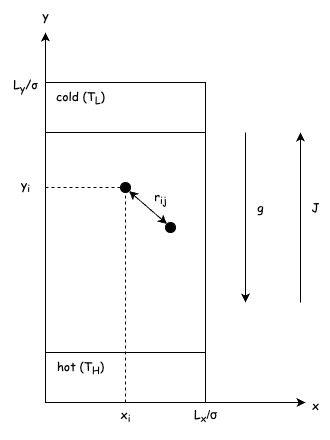
\includegraphics[scale=0.7]{image/system.jpg}
\end{figure}

\subsection{ハミルトニアン}

結論は, 

\begin{align}
  \label{Hamiltonian}
  H(\Gamma; g)
  &= \sum_{i=1}^{N}
  \left[
    \frac{{\bm{p}_i}^2}{2m} 
    + \sum_{j > i}^{N}
      \tilde{\phi}_{\text{LJ}}^{\text{pair}}(r_{ij})
    + mgy_i
    + V^{\text{wall}} (y_i)
  \right]
\end{align}

以降, 本節はこれに至るまでの過程を述べる.

\subsubsection{粒子-粒子間相互作用ポテンシャル}

シミュレーションを行う際に, 典型的な粒子間相互作用ポテンシャルとして, 12-6 Lennard-Jones Potential を採用する.

\begin{align}
  \phi_{\text{LJ}}^{\text{pair}}(r; \varepsilon, \sigma) = 4\varepsilon \qty[\qty(\frac{\sigma}{r})^{12} - \qty(\frac{\sigma}{r})^{6} ] \\
\end{align}

シミュレーション上では, カットオフ長 $r_{\text{cut}}^{\text{pair}}=3\sigma$ とポテンシャルのシフトアップを考慮して

\begin{align}
  \tilde{\phi}_{\text{LJ}}^{\text{pair}}(r;r_{\text{cut}}^{\text{pair}}) = \qty{\phi_{\text{LJ}}^{\text{pair}}(r) - \phi_{\text{LJ}}^{\text{pair}}(r_{\text{cut}}^{\text{pair}})}\theta \qty(r_{\text{cut}}^{\text{pair}}-r) \\
\end{align}

のように書き換えたポテンシャルを用いている.

\subsubsection{周期境界条件と最近接イメージ規約\cite{MD}}

周期境界条件を考慮すると, 粒子-粒子間相互ポテンシャルの総計はまず以下のように書ける.

\begin{align}
  \sum_{n_x \in \mathbb{Z}} \sum_{i=1}^{N} \sum_{\substack{j=1 \\ (j \neq i \ \text{for} \ n_{x} = 0)}}^{N} \frac{1}{2} \phi_{\text{LJ}}^{\text{pair}}(|\bm{r}_i -(\bm{r}_j + L_x \bm{e}_x)|)
\end{align}

ここで, $n_x = 0$; オリジナルセルの中では, 同じ$i,\ j$ペアのポテンシャルエネルギーを2回足すことになるので, ポテンシャルを$1/2$している. その上で, $j = i$の場合は自分自身との相互作用になるため, これは除外する. $n_x \neq 0$の場合, 粒子$j$はイメージ粒子となるため, $j=i$の場合も含めることになる. このときにもダブルカウントがあるので, ポテンシャルを$1/2$している. 

\begin{figure}[H]
  \centering
  \caption{}
  \label{fig:system_periodic}
  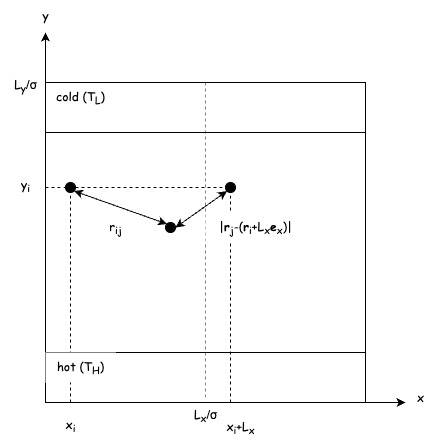
\includegraphics[scale=0.7]{image/system_periodic.jpg}
\end{figure}

注目する系の粒子が常にオリジナルセルの中にとどまっているかのようにMD上で扱うには,

\begin{align}
  x_{i} = x_{i}' \mod L_{x}
\end{align}

のように,  飛び出した粒子の$x$座標$x_{i}'$を上式のように$x_i$にシフトすれば良い. しかし, 周期境界条件とセットに, 最近接イメージ規約として, 粒子$i$がオリジナル粒子と各イメージ粒子の中で最も近い粒子$j$らとのみ相互作用をすることを課すと, 粒子間の相互ポテンシャルの総計は先ほどよりも簡単に書けるようになる.

\begin{align}
  \sum_{i=1}^{N} \sum_{j > i}^{N} \phi_{\text{LJ}}^{\text{pair}} (r_{ij})
\end{align}

\subsubsection{壁-粒子間相互作用ポテンシャル}

\begin{align}
  \phi_{\text{LJ}}^{\text{wall}}(r; \varepsilon^{\text{wall}}, \sigma^{\text{wall}}) = 4\varepsilon^{\text{wall}} \qty[\qty(\frac{\sigma^{\text{wall}}}{r})^{12} - \qty(\frac{\sigma^{\text{wall}}}{r})^{6} ] \\
\end{align}

パラメータは以下のようにする.

\begin{align}
  \varepsilon^{\text{wall}} &= \qty(1.0 - \text{R}_\text{d}) \times \varepsilon \\
  \sigma^{\text{wall}} &= \qty(0.5 + \text{R}_\text{t}) \times \sigma \\
  r^{\text{wall}}_{\text{cut}} &= \qty(2^{1/6} + \text{R}_\text{a}) \times \sigma^{\text{wall}}
\end{align}

カットオフ長とシフトアップを考慮して

\begin{align}
  \tilde{\phi}_{\text{LJ}}^{\text{wall}}(r;r_{\text{cut}}^{\text{wall}}) = \qty{\phi_{\text{LJ}}^{\text{wall}}(r) - \phi_{\text{LJ}}^{\text{wall}}(r_{\text{cut}}^{\text{wall}})}\theta \qty(r_{\text{cut}}^{\text{wall}}-r) \\
\end{align}

この系では, $y$軸方向垂直に壁がついている. よって, 壁ポテンシャルは

\begin{align}
  V^{\text{wall}}(y; L_y) &= \tilde{\phi}_{\text{LJ}}^{\text{wall}}(y;r_{\text{cut}}^{\text{wall}}) + \tilde{\phi}_{\text{LJ}}^{\text{wall}}(L_y - y;r_{\text{cut}}^{\text{wall}})
\end{align}

のように書ける. これまでのことより, ハミルトニアンは以下のように書き表せる.

\begin{align}
    H(\Gamma; g)
    &= \sum_{i=1}^{N}
    \left[
      \frac{{\bm{p}_i}^2}{2m} 
      + \sum_{j > i}^{N}
        \tilde{\phi}_{\text{LJ}}^{\text{pair}}(r_{ij})
      + mgy_i +V^{\text{wall}}(y_i)
    \right] \ \tag*{\eqref{Hamiltonian}} 
\end{align}

\subsection{熱流}

langevin熱浴に侵入した粒子に対しては, brownian 動力学計算を実行する. その粒子$i$にはたらく力$\bm{F}_i$は\href{https://docs.lammps.org/fix_langevin.html}{LAMMPSのドキュメント}に則った形式だと以下のように書き表せる.

\begin{align}
  \bm{F}_i &= \bm{F}_i^c + \bm{F}_i^f + \bm{F}_i^r \\
  \bm{F}_i^c &= - \bm{\nabla} 
  \left[
    \sum_{j > i}^{N}
        \tilde{\phi}_{\text{LJ}}^{\text{pair}}(r_{ij})
      + mgy_i +V^{\text{wall}}(y_i)
  \right]  \\
  \bm{F}_i^f &= -\frac{m_i}{\text{damp}}\bm{v}_i \\
  F_i^r &\propto \sqrt{\frac{k_\text{B} Tm_i}{dt \text{damp}}}
\end{align}

それぞれの力の説明を記す.

\begin{itemize}
  \item $\bm{F}^c$; ポテンシャルを介して計算される力
  \item $\bm{F}^f$; 摩擦力
  \item $\bm{F}^r$; ランダム力
\end{itemize}


\subsubsection{温度制御}


2d kinetic temperature

\begin{align}
  T \equiv \frac{1}{Nk_{\text{B}}}\sum_{i=1}^{N} \frac{1}{2}m_i v_{i}^2
\end{align}

粒子$i$が熱浴に侵入すると, その粒子の運動はランジュバン方程式に従う. 侵入していないときは, $\gamma = 0$になり, 正準方程式に等しくなる.

\begin{align}
  \dot{\bm{r}_i} &= \pdv{H}{\bm{p}_i} \\
  \dot{\bm{p}_i} &= - \pdv{H}{\bm{r}_i} - \gamma \dot{\bm{r}_i} + \sqrt{2 \gamma k_{\text{B}}T_{\nu}}\bm{\xi}_i (t) \\
  \expval{\xi_{i}^{a}(t)} &= 0 \\
  \expval{\xi_{i}^{a}(t)\xi_{j}^{b}(t')} &= \delta_{i,j} \delta_{a,b}\delta (t-t') 
\end{align}

\begin{align}
  \gamma(y_i) &= 1. \ T_{\nu}(y_i) = T_{\text{H}}. \ (0 < y_i < 8\sigma) \\
  \gamma(y_i) &= 1. \ T_{\nu}(y_i) = T_{\text{L}}. \ (L_y - 8\sigma < y_i < L_y) \\
  \gamma(y_i) &= 0.  \ (8\sigma < y_i < L_y - 8\sigma)
\end{align}


\section{実験}

雨が降るシミュレーションをしたい.

系の両端のポテンシャルエネルギー差$mgL_y$と運動エネルギー差$k_{\text{B}}\Delta T$の比を$\chi$として以下のように設定する.

\begin{align}
  \chi \equiv \frac{k_{\text{B}}\Delta T}{mgL_{y}} = 1.265
\end{align}

壁ポテンシャルまわりの無次元パラメータを3つ用意する.

\begin{align}
  \text{R}_\text{d} &: 乾き具合. \\
  \text{R}_\text{t} &: 壁の厚み. \\
  \text{R}_\text{a} &: 濡れ具合.
\end{align}

これを用いて, 壁-粒子間相互作用LJポテンシャルは以下のように書き表す.

\begin{align}
  \varepsilon^{\text{wall}} &= \qty(1.0 - \text{R}_\text{d}) \times \varepsilon \\
  \sigma^{\text{wall}} &= \qty(0.5 + \text{R}_\text{t}) \times \sigma \\
  r^{\text{wall}}_{\text{cut}} &= \qty(2^{1/6} + \text{R}_\text{a}) \times \sigma^{\text{wall}}
\end{align}

パラメータ $(\text{R}_\text{d}, \text{R}_\text{t}, \text{R}_\text{a})$ を変えることによって, 壁-粒子間相互作用LJポテンシャルが変わったときに, どのように粒子集団の様相が変化するかをみる. 本章の以降の実験は特記がない限り以下のパラメータに近い値で行うものとする. 

\begin{itemize}
  \item $N = 1250$
  \item $\rho {\sigma}^2 = 0.4$
  \item $L_x / \sigma = 39.5\dots$
  \item $L_y / \sigma = 79.0\dots$
  \item $k_{\text{B}} T / \varepsilon = 0.43$
  \item $k_{\text{B}} \Delta T / \varepsilon = 0.04$
  \item $mg\sigma/\varepsilon = 4.0 \times 10^{-4}$
  \item $t_f \sqrt{\varepsilon / m \sigma^2} = 1.0 \times 10^{5}$
\end{itemize}


\subsection{追実験}

壁を完全に濡らしていることを考えたいので, $r^{\text{wall}}_{\text{cut}}=1.0$ のときを考えている.

重力をかけた状態で緩和するまでシミュレーションを行っている.

\begin{itemize}
  \item $N = 5000$
  \item $\rho \sigma^2 = 0.4$
  \item $L_x / \sigma = 79.0\dots$
  \item $L_y / \sigma = 158.1\dots$
  \item $k_{\text{B}} T/\varepsilon = 4.3$
  \item $k_{\text{B}} \Delta T/\varepsilon = 0.0$
  \item $mg\sigma/\varepsilon = 2.0 \times 10^{-4}$
  \item $t_b \sqrt{\varepsilon / m \sigma^2} = 5.0 \times 10^{5}$
\end{itemize}

重力をかけた緩和後の系で, 熱浴の温度差を改めて以下のようにつけ, 熱流を流してシミュレーションをしている.

\begin{itemize}
  \item $\chi = k_{\text{B}}\Delta T / mg L_y = 1.265$
  \item $k_{\text{B}} \Delta T/\varepsilon = 0.04$
  \item $t_a \sqrt{\varepsilon / m \sigma^2} = 5.0 \times 10^{5}$
\end{itemize}

まずは, $(\text{R}_\text{d} = 0.0, \text{R}_\text{t} = 0.5, \text{R}_\text{a} = 3.0 - 2^{1/6})$ で実験を行う. これは, $(\varepsilon^{\text{wall}} = \varepsilon, \sigma^{\text{wall}} = \sigma, r^{\text{wall}}_{\text{cut}} = 3\sigma^{\text{wall}})$ に対応しているので, $\phi_{\text{LJ}} = \phi_{\text{LJ}}^{\text{wall}}$ ということになり, 先行研究と同じ結果を得るはずである.

\begin{figure}[H]
  \centering
  \href{https://youtu.be/CIEyUPvPY6A}{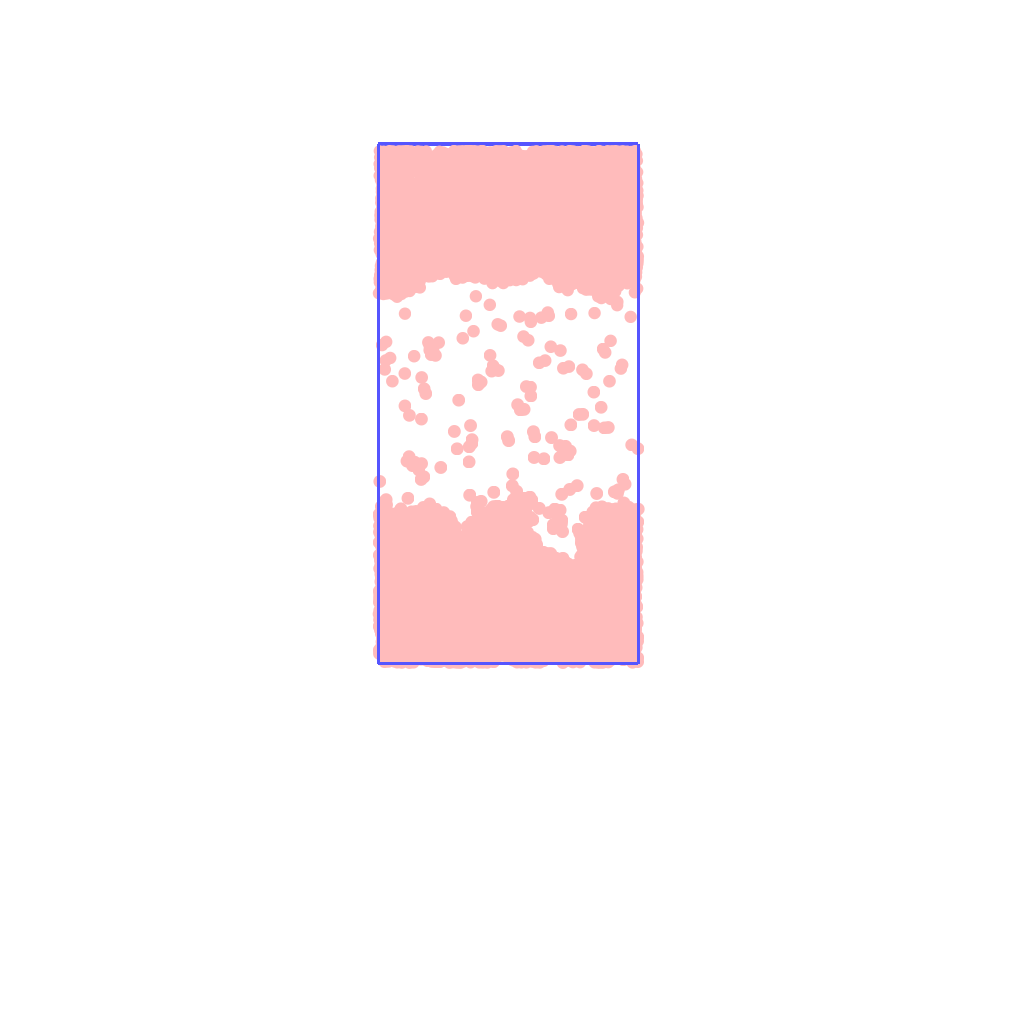
\includegraphics[scale=0.2]{image/2023-11-21T21:01:17.543_followup_chi1.265_Ay100_rho0.4_T0.43_dT0.04_Rd0.0_Rt0.5_Ra1.877538_g0.00019998593898298055_run1.0e8_output.png}}
  \caption{Ay100\_rho0.4\_T0.43\_dT0.04\_Rd0.0\_Rt0.5\_Ra1.877538\_g0.0004\_run1.0e8}
  \label{}
\end{figure}


\subsection{$\text{R}_\text{a}$, $\text{R}_\text{t}$ マップ}

\begin{align}
  \text{R}_\text{a} &= 0.0 \sim 3.0 - 2^{1/6} \\
  \text{R}_\text{t} &= 0.0 \sim 0.5
\end{align}

\begin{figure}[H]
  \centering
  \begin{tabular}{ccccc}
    \begin{minipage}[t]{0.2\hsize}
      \centering
      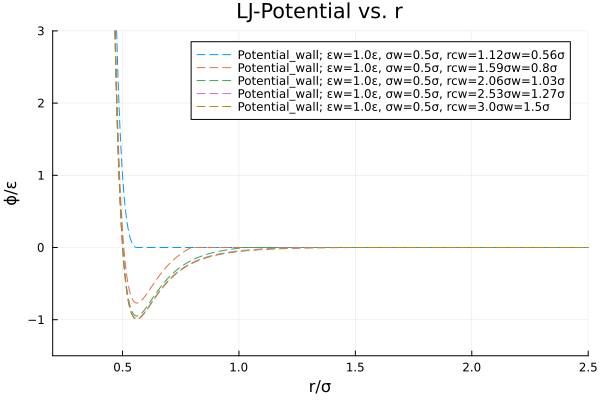
\includegraphics[width=\textwidth]{image/RaRtmap_LJ/LJ-Potential_Rt0.0.png}
      \subcaption{$\text{R}_\text{t}:0.0$}
      \label{}
    \end{minipage} &
    \begin{minipage}[t]{0.2\hsize}
      \centering
      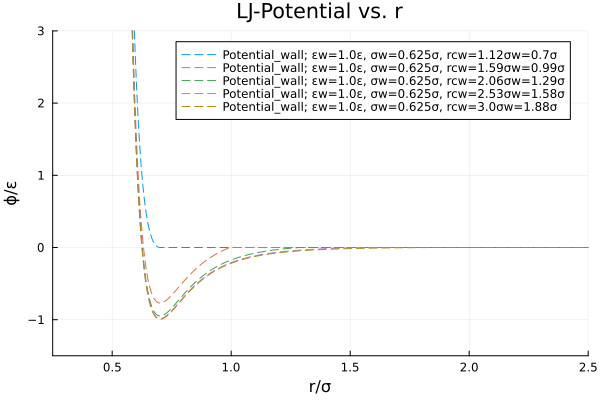
\includegraphics[width=\textwidth]{image/RaRtmap_LJ/LJ-Potential_Rt0.125.png}
      \subcaption{$\text{R}_\text{t}:0.125$}
      \label{}
    \end{minipage} &
    \begin{minipage}[t]{0.2\hsize}
      \centering
      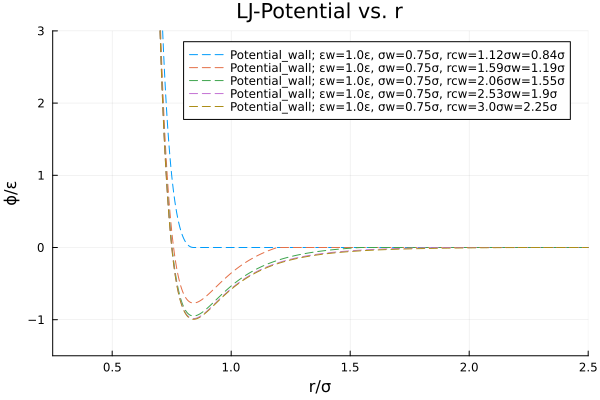
\includegraphics[width=\textwidth]{image/RaRtmap_LJ/LJ-Potential_Rt0.25.png}
      \subcaption{$\text{R}_\text{t}:0.25$}
      \label{}
    \end{minipage} &
    \begin{minipage}[t]{0.2\hsize}
      \centering
      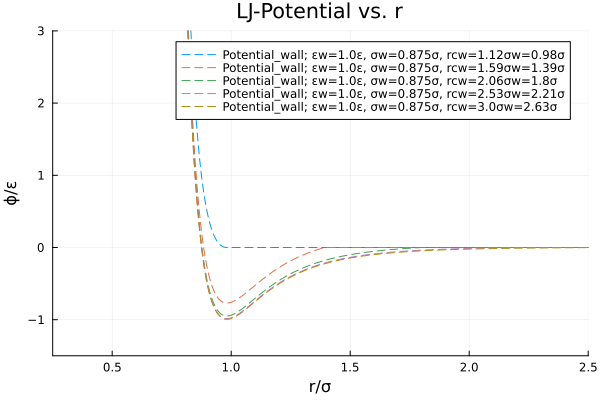
\includegraphics[width=\textwidth]{image/RaRtmap_LJ/LJ-Potential_Rt0.375.png}
      \subcaption{$\text{R}_\text{t}:0.375$}
      \label{}
    \end{minipage} &
    \begin{minipage}[t]{0.2\hsize}
      \centering
      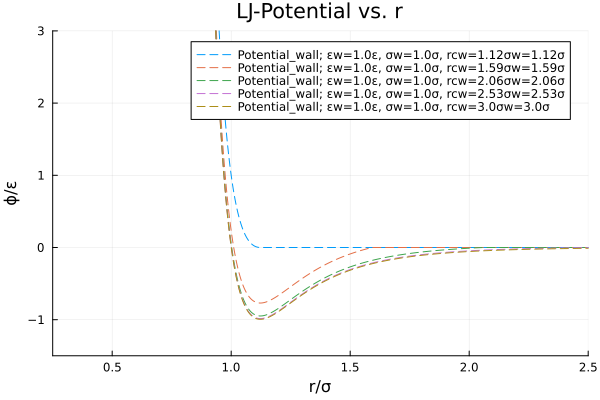
\includegraphics[width=\textwidth]{image/RaRtmap_LJ/LJ-Potential_Rt0.5.png}
      \subcaption{$\text{R}_\text{t}:0.5$}
      \label{}
    \end{minipage} 
  \end{tabular}
  \caption{LJ-potential}
  \label{}
\end{figure}

\begin{itemize}
  \item $N = 1250$
  \item $\rho {\sigma}^2 = 0.4$
  \item $L_x / \sigma = 39.5\dots$
  \item $L_y / \sigma = 79.0\dots$
  \item $k_{\text{B}} T / \varepsilon = 0.43$
  \item $k_{\text{B}} \Delta T / \varepsilon = 0.04$
  \item $mg\sigma/\varepsilon = 4.0 \times 10^{-4}$
  \item $t_f \sqrt{\varepsilon / m \sigma^2} = 2.0 \times 10^{5}$
\end{itemize}

\begin{figure}[H]
  \begin{tabular}{ccccc}
    \begin{minipage}[t]{0.2\hsize}
      \centering
      \href{https://youtu.be/yc-GeIQBuCk}{
\includegraphics[width=\textwidth]{image/RaRtmap/2023-11-14T18:19:29.358__chi1.265_Ay50_rho0.4_T0.43_dT0.04_Rd0.0_Rt0.0_Ra0.0_g0.0003999718779659611_run4.0e7_output.png}}
      \subcaption{$\text{R}_\text{a}=0.0,\\\text{R}_\text{t}=0.0$}
      % \label{}
    \end{minipage} &
    \begin{minipage}[t]{0.2\hsize}
      \centering
      \href{https://youtu.be/4rNNLx9_DZ4}{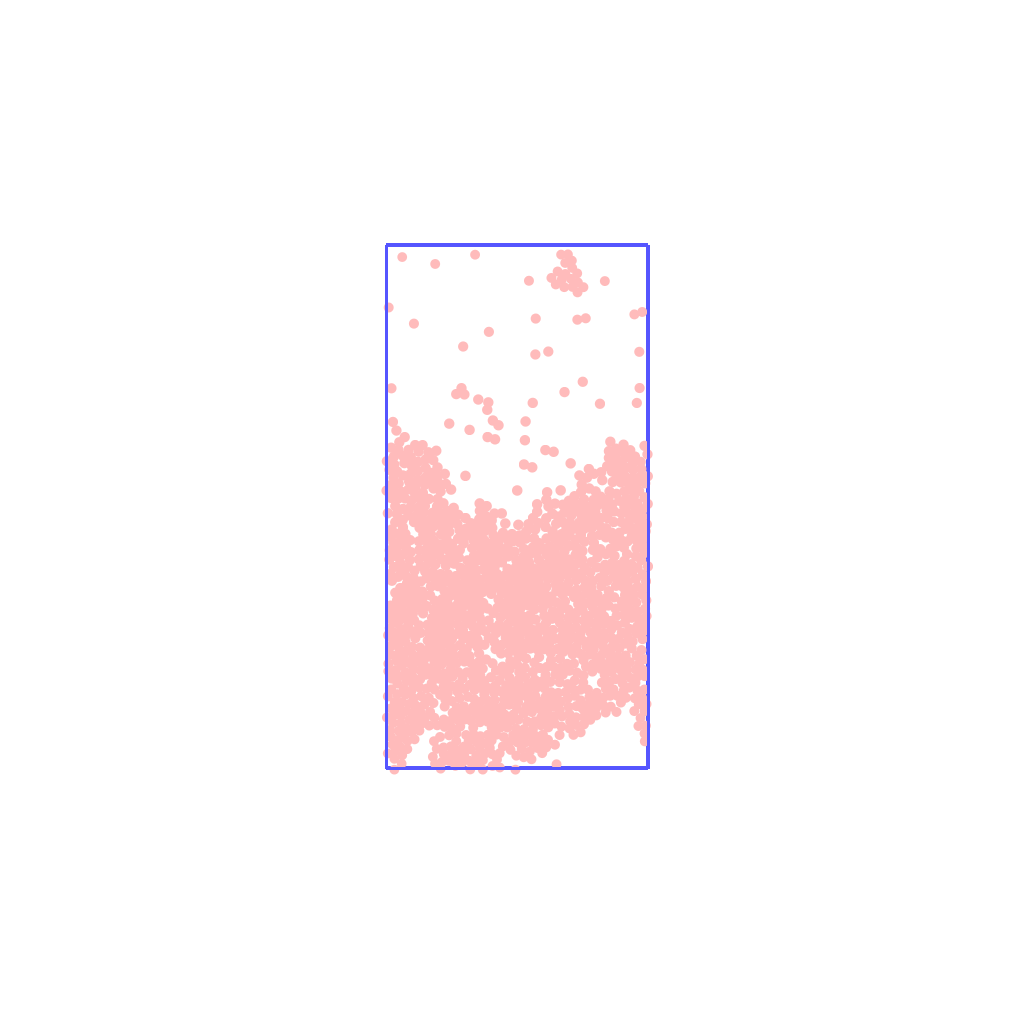
\includegraphics[width=\textwidth]{image/RaRtmap/2023-11-14T19:14:52.710__chi1.265_Ay50_rho0.4_T0.43_dT0.04_Rd0.0_Rt0.0_Ra0.4693845_g0.0003999718779659611_run4.0e7_output.png}}
      \subcaption{$\text{R}_\text{a}=0.469,\\\text{R}_\text{t}=0.0$}
      % \label{}
    \end{minipage} &
    \begin{minipage}[t]{0.2\hsize}
      \centering
      \href{https://youtu.be/QKLz7NzBte8}{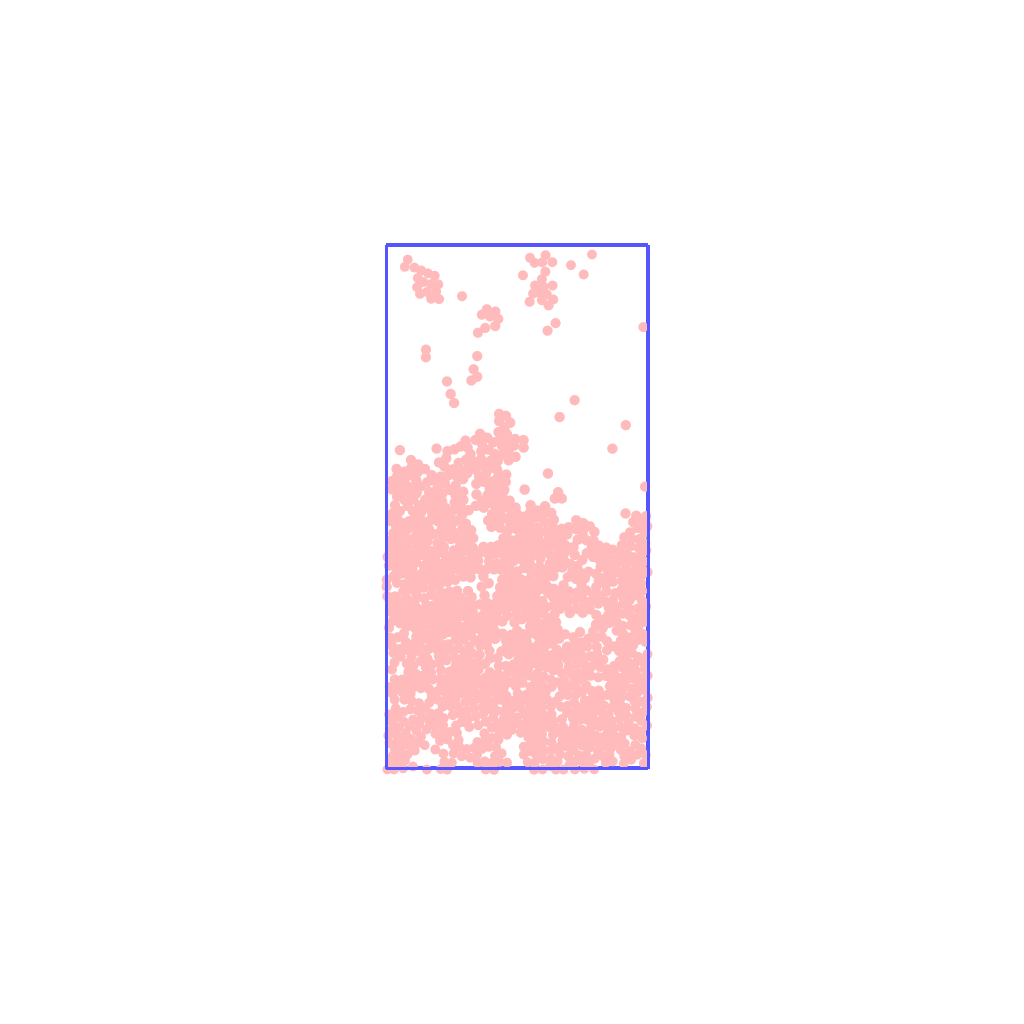
\includegraphics[width=\textwidth]{image/RaRtmap/2023-11-14T20:07:58.625__chi1.265_Ay50_rho0.4_T0.43_dT0.04_Rd0.0_Rt0.0_Ra0.938769_g0.0003999718779659611_run4.0e7_output.png}}
      \subcaption{$\text{R}_\text{a}=0.938,\\\text{R}_\text{t}=0.0$}
      % \label{}
    \end{minipage} &
    \begin{minipage}[t]{0.2\hsize}
      \centering
      \href{https://youtu.be/6iqcv_Af2U8}{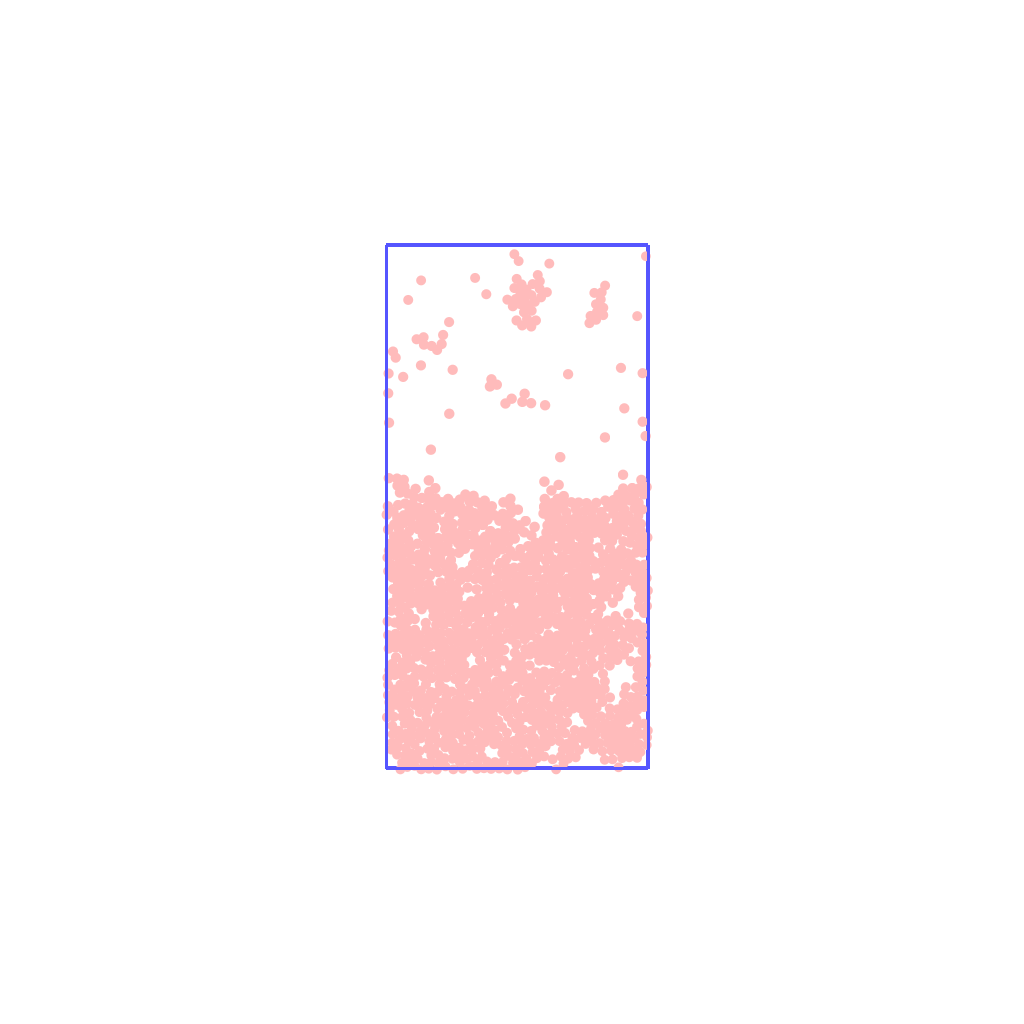
\includegraphics[width=\textwidth]{image/RaRtmap/2023-11-14T21:01:09.992__chi1.265_Ay50_rho0.4_T0.43_dT0.04_Rd0.0_Rt0.0_Ra1.4081535_g0.0003999718779659611_run4.0e7_output.png}}
      \subcaption{$\text{R}_\text{a}=1.408,\\\text{R}_\text{t}=0.0$}
      % \label{}
    \end{minipage} &
    \begin{minipage}[t]{0.2\hsize}
      \centering
      \href{https://youtu.be/Tn1Hd2eR0yo}{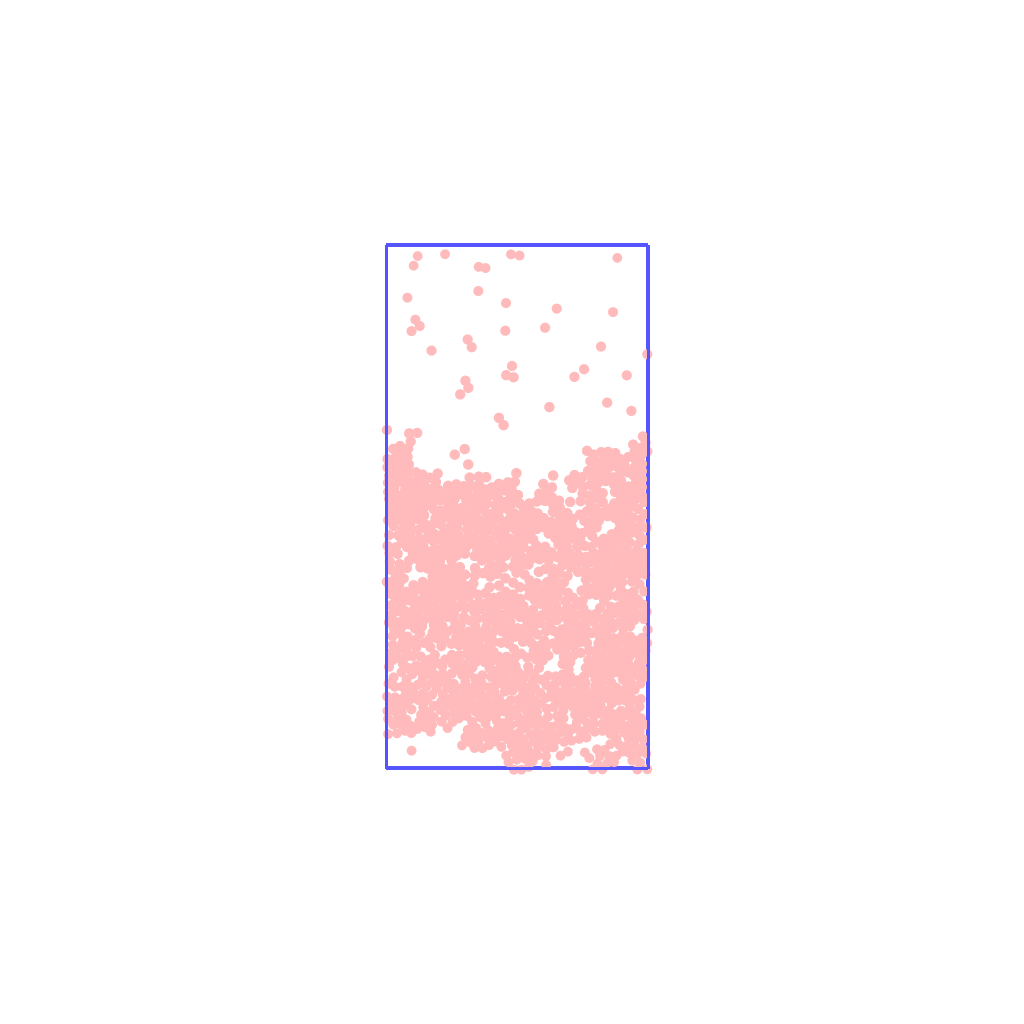
\includegraphics[width=\textwidth]{image/RaRtmap/2023-11-14T21:54:59.835__chi1.265_Ay50_rho0.4_T0.43_dT0.04_Rd0.0_Rt0.0_Ra1.877538_g0.0003999718779659611_run4.0e7_output.png}}
      \subcaption{$\text{R}_\text{a}=1.877,\\\text{R}_\text{t}=0.0$}
      % \label{}
    \end{minipage} \\
    \begin{minipage}[t]{0.2\hsize}
      \centering
      \href{https://youtu.be/B1GwQFCBszs}{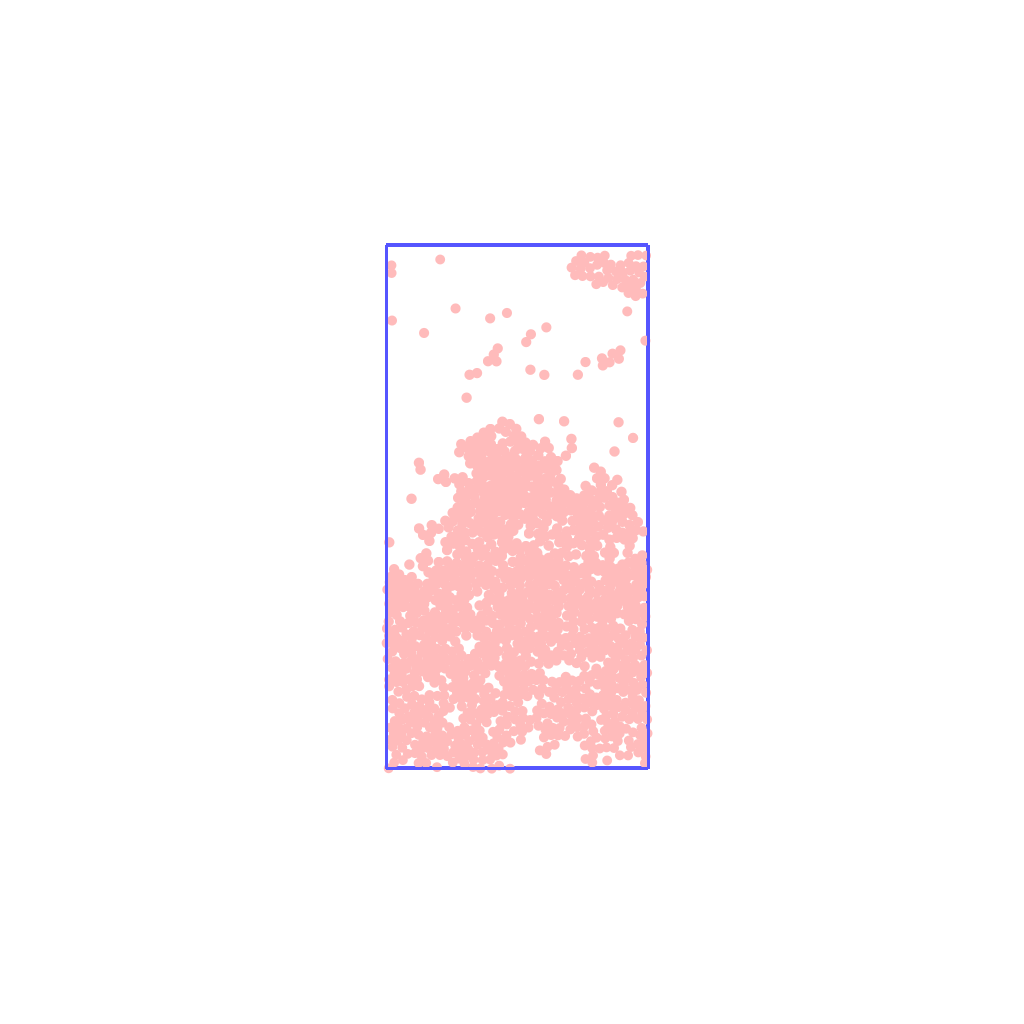
\includegraphics[width=\textwidth]{image/RaRtmap/2023-11-14T22:51:24.191__chi1.265_Ay50_rho0.4_T0.43_dT0.04_Rd0.0_Rt0.125_Ra0.0_g0.0003999718779659611_run4.0e7_output.png}}
      \subcaption{$\text{R}_\text{a}=0.0,\\\text{R}_\text{t}=0.125$}
      % \label{}
    \end{minipage} &
    \begin{minipage}[t]{0.2\hsize}
      \centering
      \href{https://youtu.be/MRIfAketXOI}{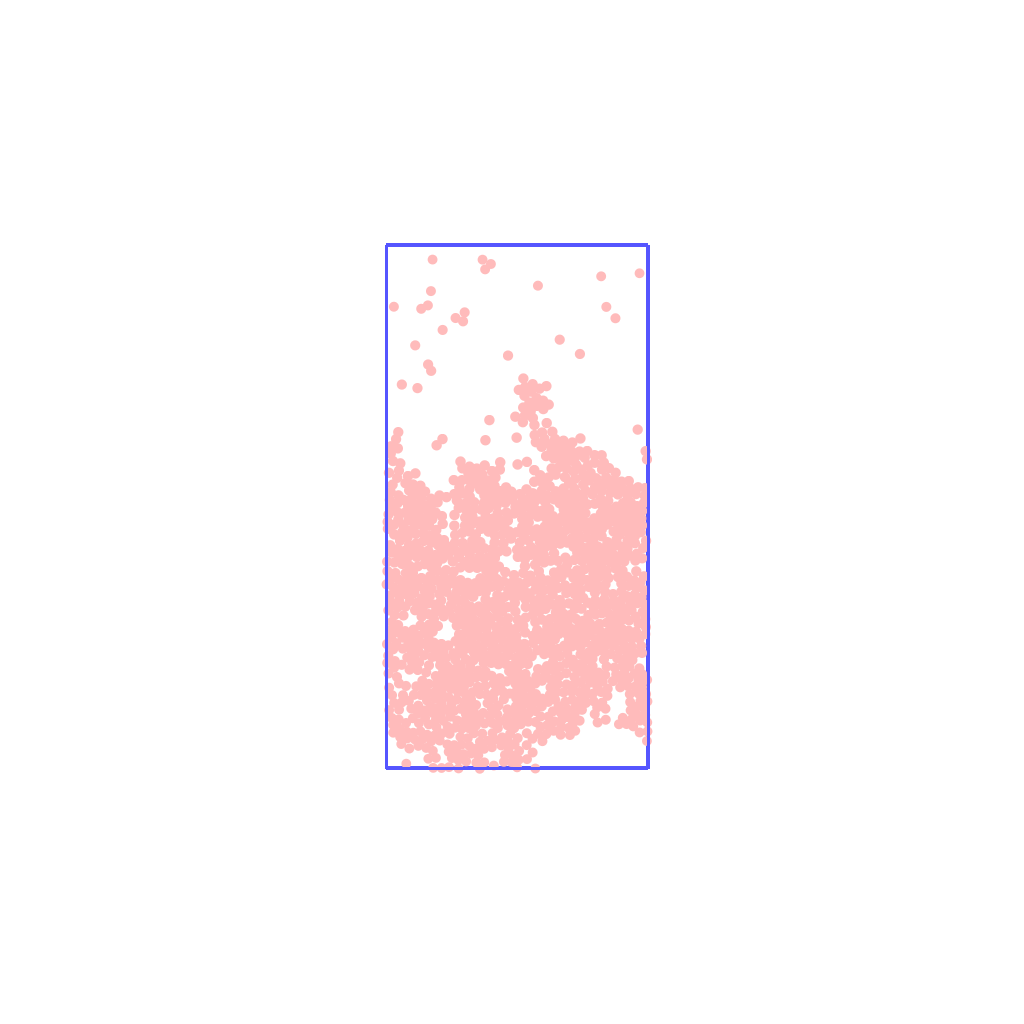
\includegraphics[width=\textwidth]{image/RaRtmap/2023-11-14T23:48:31.439__chi1.265_Ay50_rho0.4_T0.43_dT0.04_Rd0.0_Rt0.125_Ra0.4693845_g0.0003999718779659611_run4.0e7_output.png}}
      \subcaption{$\text{R}_\text{a}=0.469,\\\text{R}_\text{t}=0.125$}
      % \label{}
    \end{minipage} &
    \begin{minipage}[t]{0.2\hsize}
      \centering
      \href{https://youtu.be/v7rYxdoSSjI}{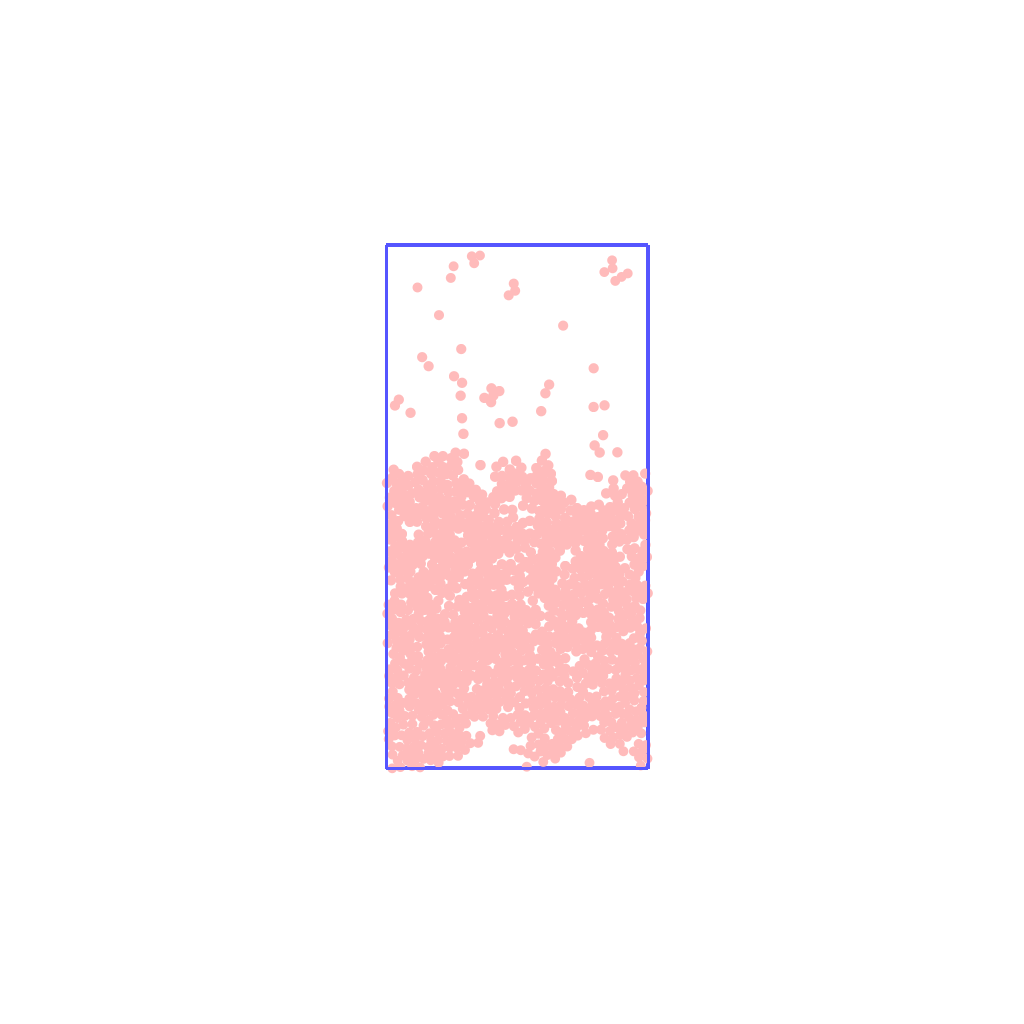
\includegraphics[width=\textwidth]{image/RaRtmap/2023-11-15T00:43:33.781__chi1.265_Ay50_rho0.4_T0.43_dT0.04_Rd0.0_Rt0.125_Ra0.938769_g0.0003999718779659611_run4.0e7_output.png}}
      \subcaption{$\text{R}_\text{a}=0.938,\\\text{R}_\text{t}=0.125$}
      % \label{}
    \end{minipage} &
    \begin{minipage}[t]{0.2\hsize}
      \centering
      \href{https://youtu.be/0NFYPFYBcc4}{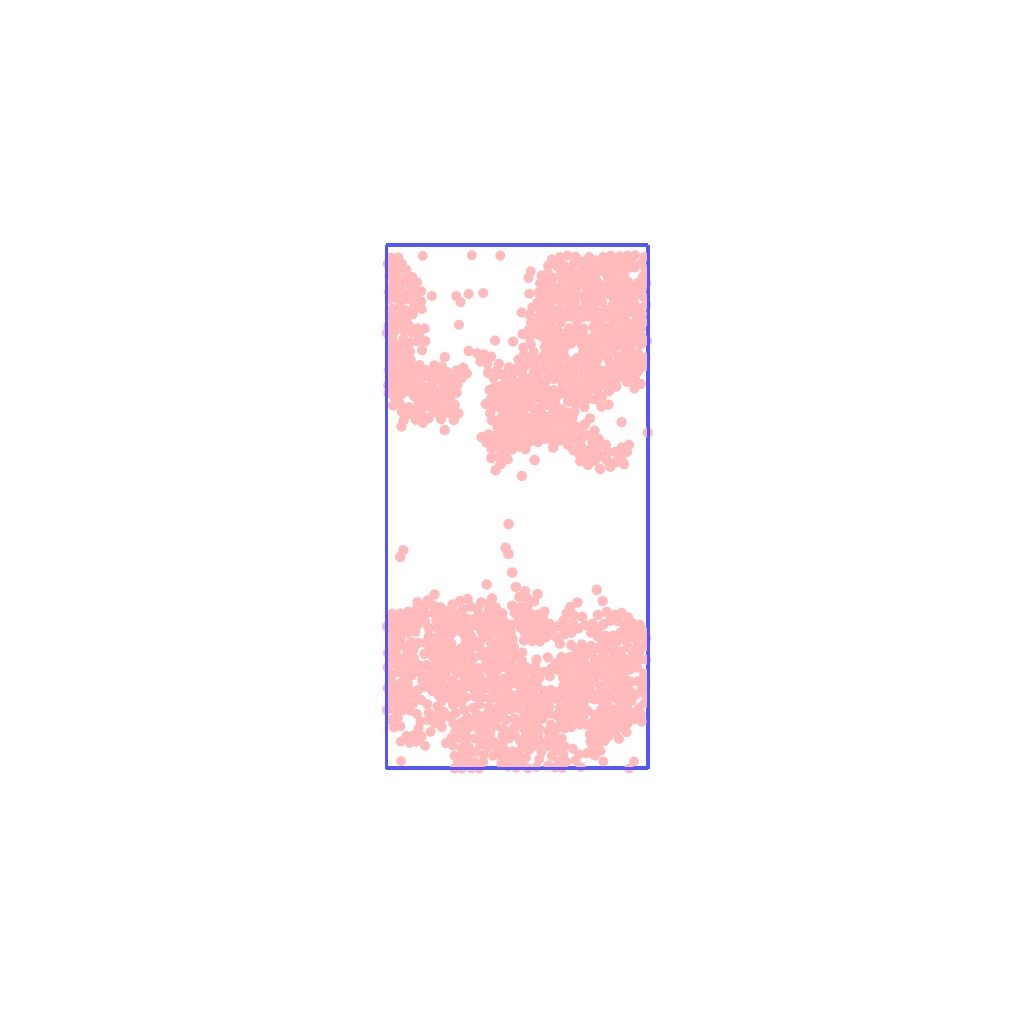
\includegraphics[width=\textwidth]{image/RaRtmap/2023-11-15T01:35:17.404__chi1.265_Ay50_rho0.4_T0.43_dT0.04_Rd0.0_Rt0.125_Ra1.4081535_g0.0003999718779659611_run4.0e7_output.png}}
      \subcaption{$\text{R}_\text{a}=1.408,\\\text{R}_\text{t}=0.125$}
      % \label{}
    \end{minipage} &
    \begin{minipage}[t]{0.2\hsize}
      \centering
      \href{https://youtu.be/FXTDOcpARl0}{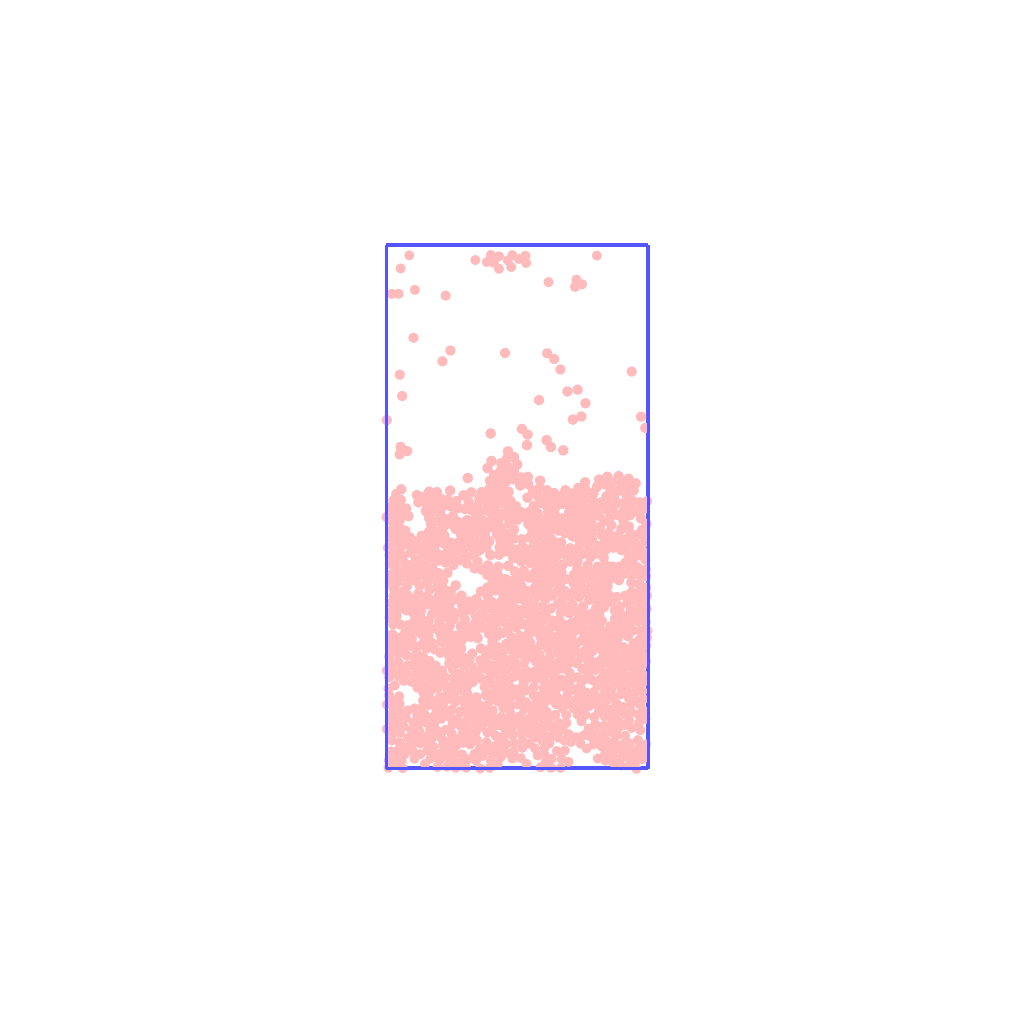
\includegraphics[width=\textwidth]{image/RaRtmap/2023-11-15T02:27:34.337__chi1.265_Ay50_rho0.4_T0.43_dT0.04_Rd0.0_Rt0.125_Ra1.877538_g0.0003999718779659611_run4.0e7_output.png}}
      \subcaption{$\text{R}_\text{a}=1.877,\\\text{R}_\text{t}=0.125$}
      % \label{}
    \end{minipage} \\
    \begin{minipage}[t]{0.2\hsize}
      \centering
      \href{https://youtu.be/4A\_MHNHZrKQ}{
      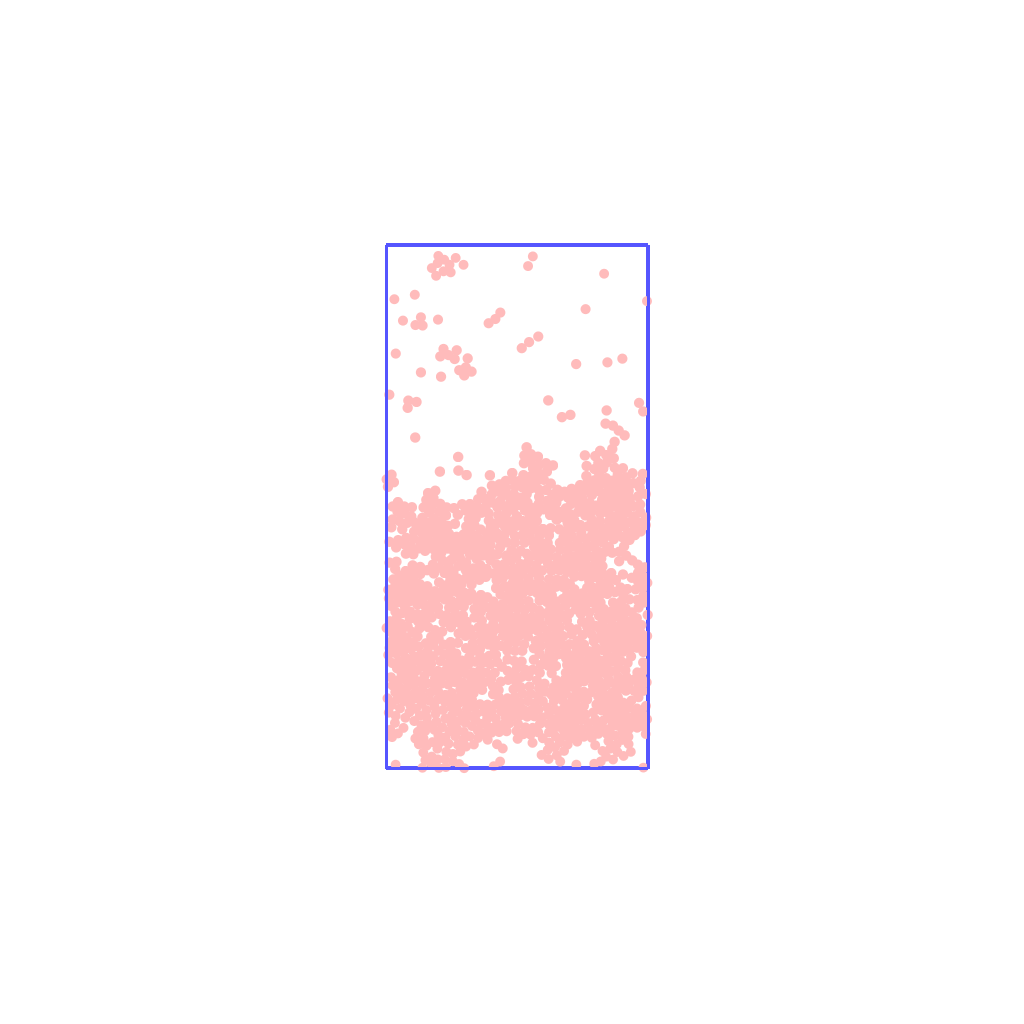
\includegraphics[width=\textwidth]{image/RaRtmap/2023-11-15T03:19:32.715__chi1.265_Ay50_rho0.4_T0.43_dT0.04_Rd0.0_Rt0.25_Ra0.0_g0.0003999718779659611_run4.0e7_output.png}}
      \subcaption{$\text{R}_\text{a}=0.0,\\\text{R}_\text{t}=0.250$}
      % \label{}
    \end{minipage} &
    \begin{minipage}[t]{0.2\hsize}
      \centering
      \href{https://youtu.be/jGzUPm\_3oH0}{
      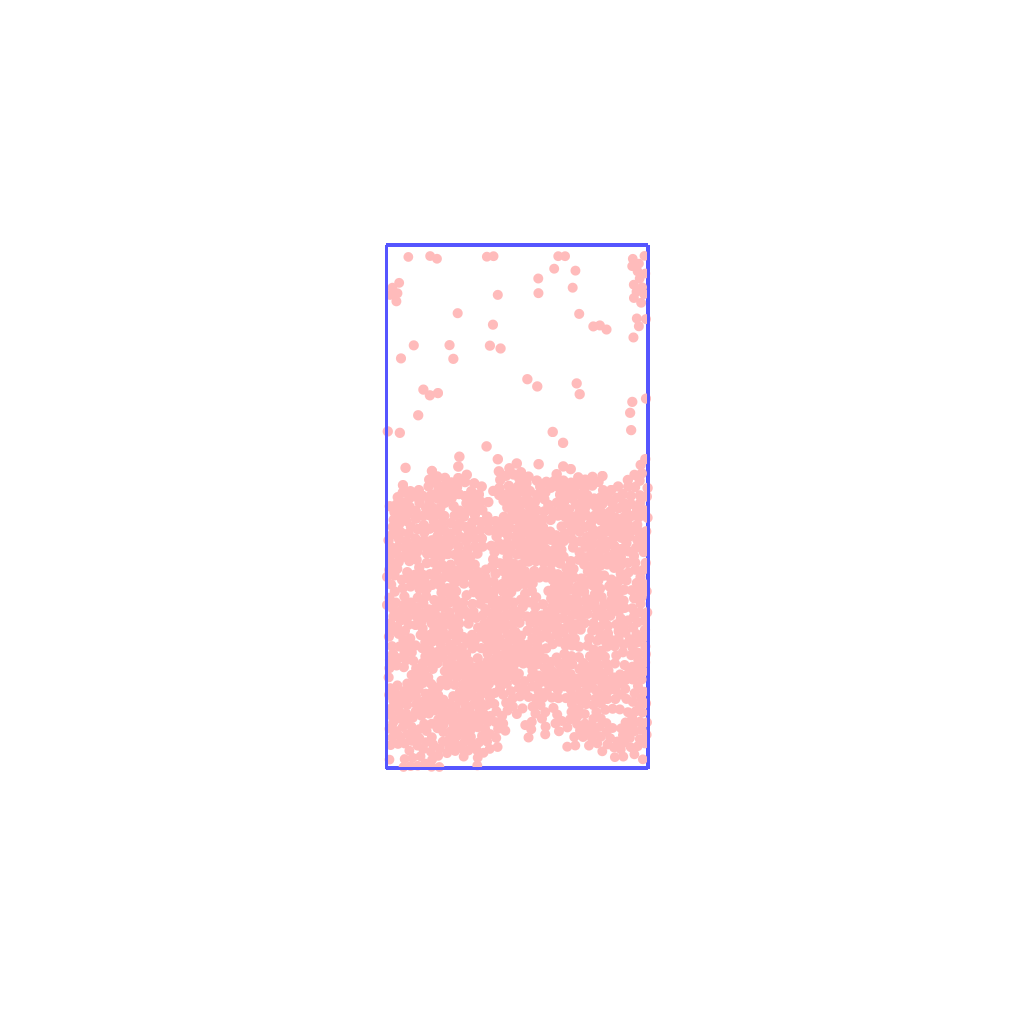
\includegraphics[width=\textwidth]{image/RaRtmap/2023-11-15T04:11:00.956__chi1.265_Ay50_rho0.4_T0.43_dT0.04_Rd0.0_Rt0.25_Ra0.4693845_g0.0003999718779659611_run4.0e7_output.png}}
      \subcaption{$\text{R}_\text{a}=0.469,\\\text{R}_\text{t}=0.250$}
      % \label{}
    \end{minipage} &
    \begin{minipage}[t]{0.2\hsize}
      \centering
      \href{https://youtu.be/0iyDEBwDF7A}{
      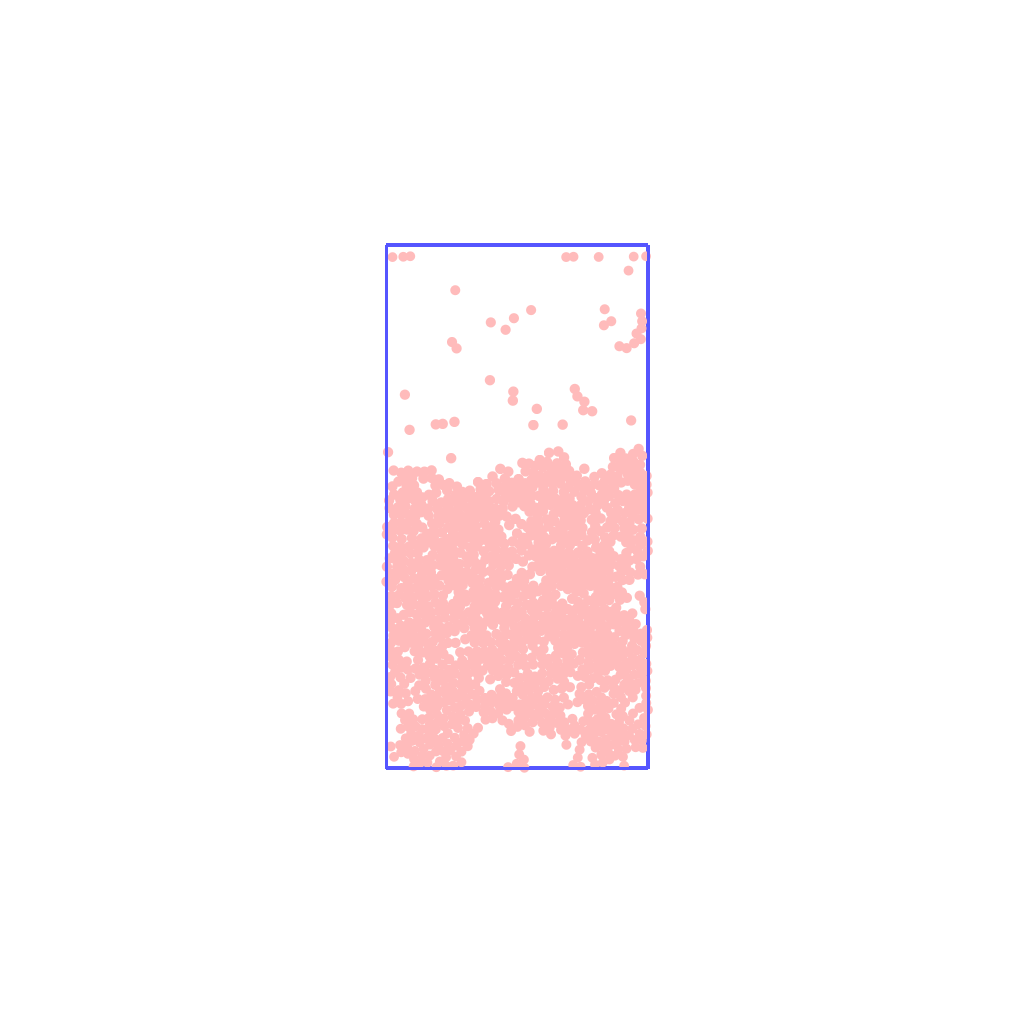
\includegraphics[width=\textwidth]{image/RaRtmap/2023-11-15T05:03:45.973__chi1.265_Ay50_rho0.4_T0.43_dT0.04_Rd0.0_Rt0.25_Ra0.938769_g0.0003999718779659611_run4.0e7_output.png}}
      \subcaption{$\text{R}_\text{a}=0.938,\\\text{R}_\text{t}=0.250$}
      % \label{}
    \end{minipage} &
    \begin{minipage}[t]{0.2\hsize}
      \centering
      \href{https://youtu.be/Sqk3HDSDINw}{
      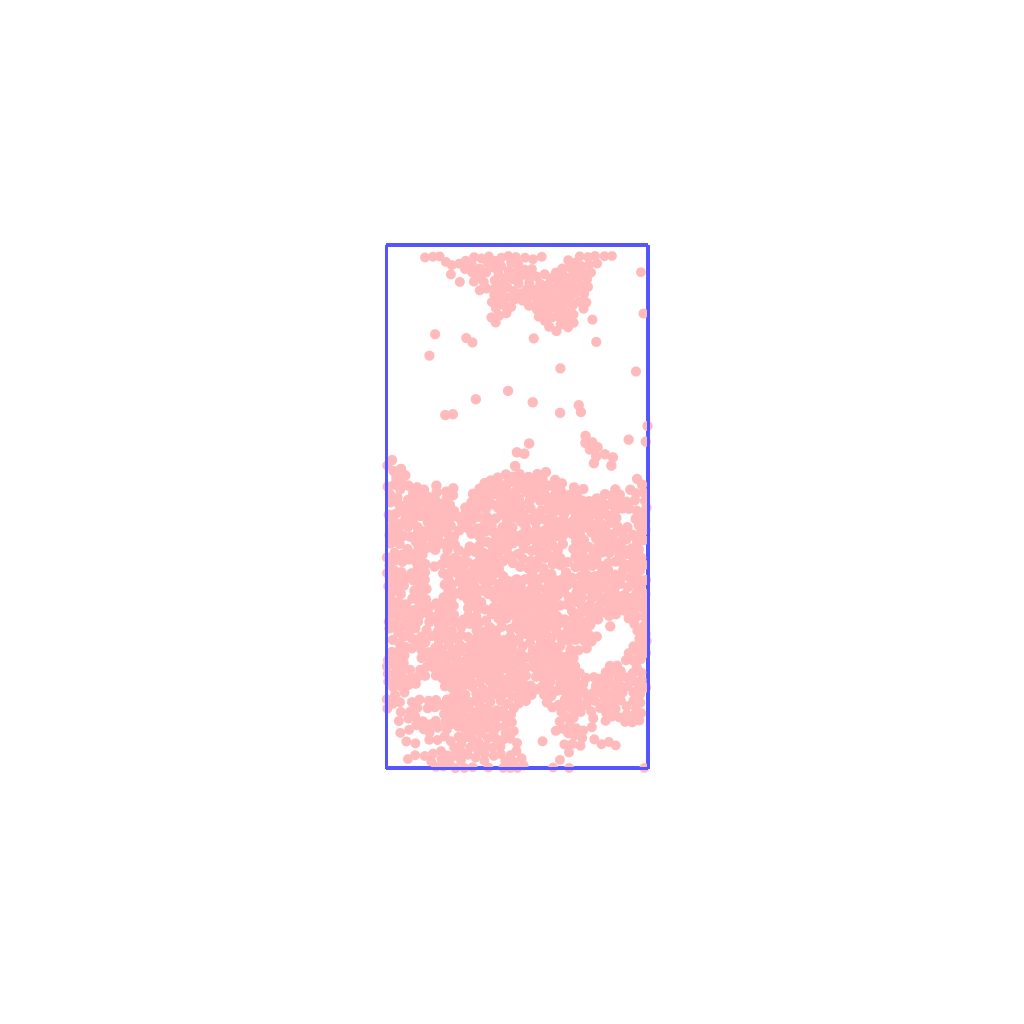
\includegraphics[width=\textwidth]{image/RaRtmap/2023-11-15T05:53:00.667__chi1.265_Ay50_rho0.4_T0.43_dT0.04_Rd0.0_Rt0.25_Ra1.4081535_g0.0003999718779659611_run4.0e7_output.png}}
      \subcaption{$\text{R}_\text{a}=1.408,\\\text{R}_\text{t}=0.250$}
      % \label{}
    \end{minipage} &
    \begin{minipage}[t]{0.2\hsize}
      \centering
      \href{https://youtu.be/3lqCLQchVYA}{
      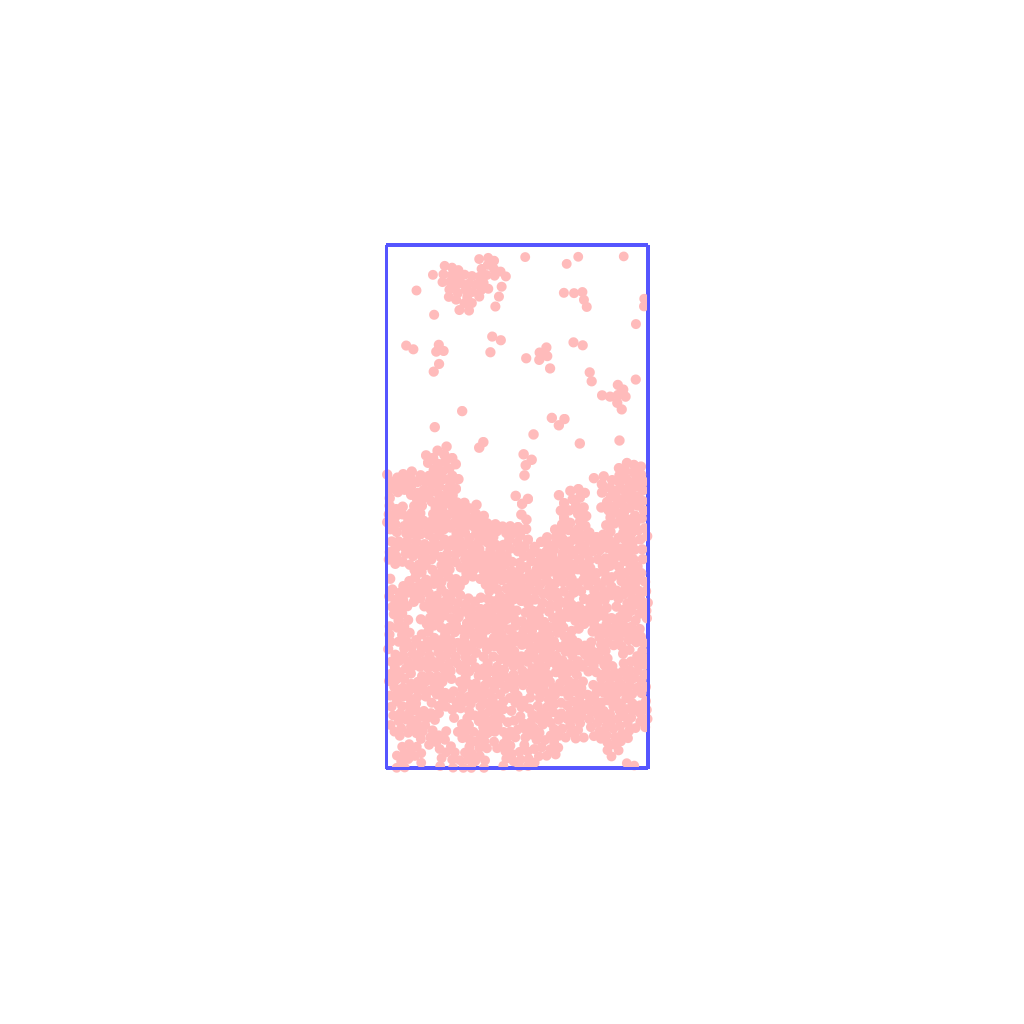
\includegraphics[width=\textwidth]{image/RaRtmap/2023-11-15T06:43:21.554__chi1.265_Ay50_rho0.4_T0.43_dT0.04_Rd0.0_Rt0.25_Ra1.877538_g0.0003999718779659611_run4.0e7_output.png}}
      \subcaption{$\text{R}_\text{a}=1.877,\\\text{R}_\text{t}=0.250$}
      % \label{}
    \end{minipage} \\
    \begin{minipage}[t]{0.2\hsize}
      \centering
      \href{https://youtu.be/1cMmZVmcThA}{
      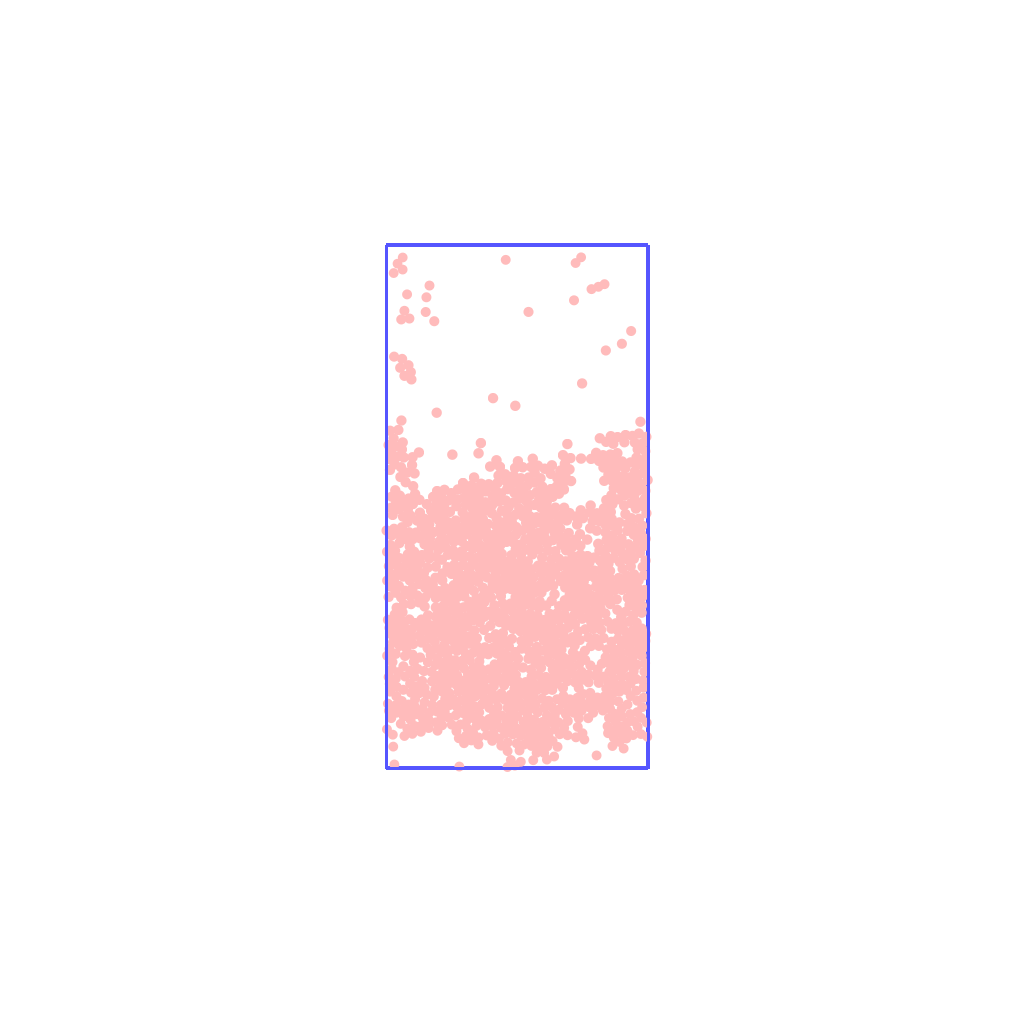
\includegraphics[width=\textwidth]{image/RaRtmap/2023-11-15T07:34:00.555__chi1.265_Ay50_rho0.4_T0.43_dT0.04_Rd0.0_Rt0.375_Ra0.0_g0.0003999718779659611_run4.0e7_output.png}}
      \subcaption{$\text{R}_\text{a}=0.0,\\\text{R}_\text{t}=0.375$}
      % \label{}
    \end{minipage} &
    \begin{minipage}[t]{0.2\hsize}
      \centering
      \href{https://youtu.be/MDWWS7Axo-4}{
      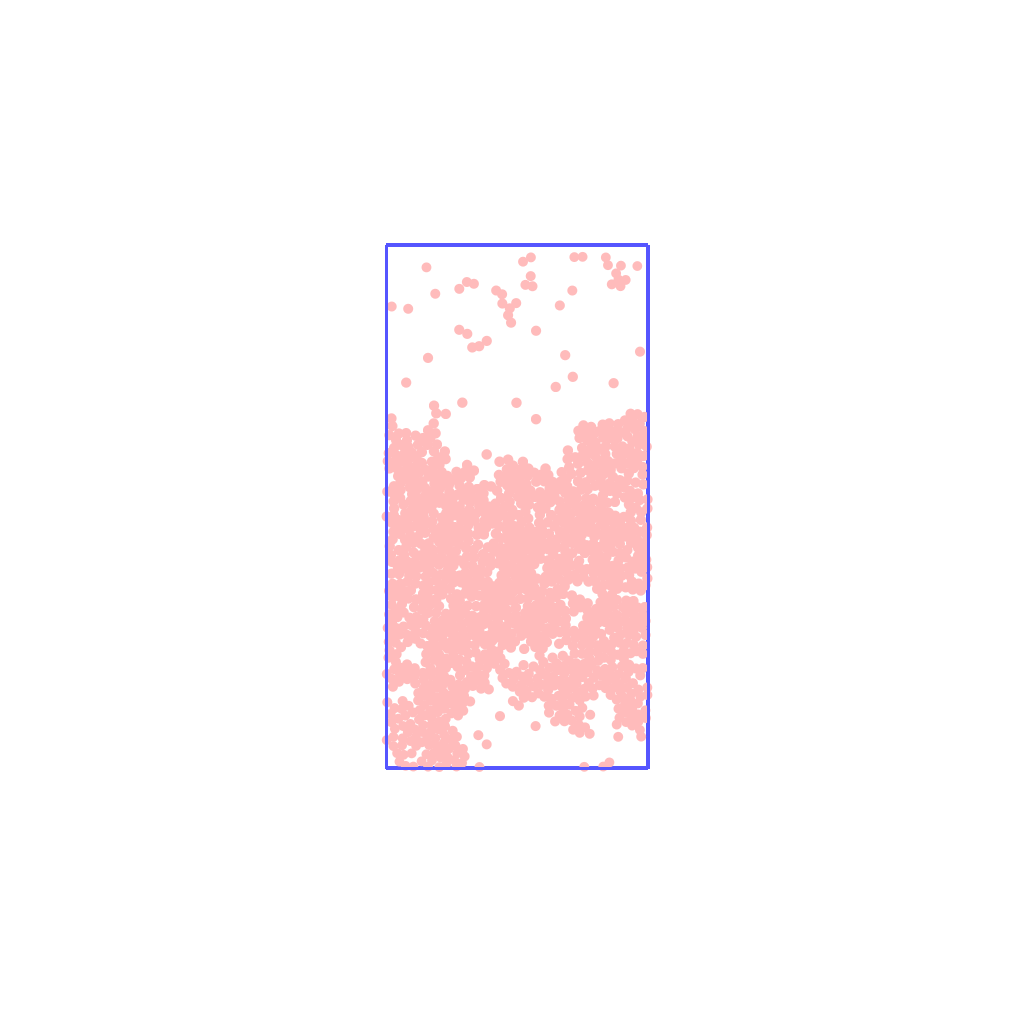
\includegraphics[width=\textwidth]{image/RaRtmap/2023-11-15T08:24:37.362__chi1.265_Ay50_rho0.4_T0.43_dT0.04_Rd0.0_Rt0.375_Ra0.4693845_g0.0003999718779659611_run4.0e7_output.png}}
      \subcaption{$\text{R}_\text{a}=0.469,\\\text{R}_\text{t}=0.375$}
      % \label{}
    \end{minipage} &
    \begin{minipage}[t]{0.2\hsize}
      \centering
      \href{https://youtu.be/Y6O_tVs6mHY}{
      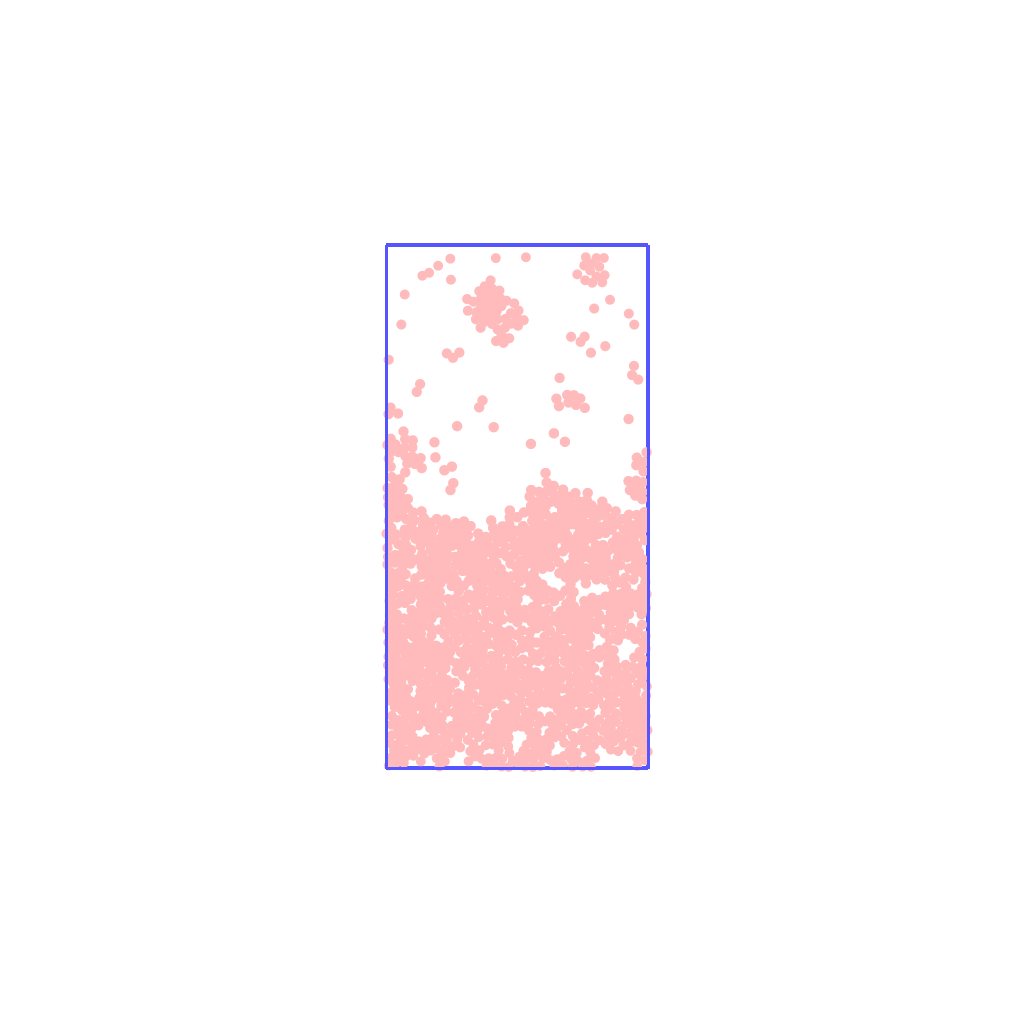
\includegraphics[width=\textwidth]{image/RaRtmap/2023-11-15T09:16:40.082__chi1.265_Ay50_rho0.4_T0.43_dT0.04_Rd0.0_Rt0.375_Ra0.938769_g0.0003999718779659611_run4.0e7_output.png}}
      \subcaption{$\text{R}_\text{a}=0.938,\\\text{R}_\text{t}=0.375$}
      % \label{}
    \end{minipage} &
    \begin{minipage}[t]{0.2\hsize}
      \centering
      \href{https://youtu.be/yeI5CDT0TEw}{
      
\includegraphics[width=\textwidth]{image/RaRtmap/2023-11-15T10:07:20.945__chi1.265_Ay50_rho0.4_T0.43_dT0.04_Rd0.0_Rt0.375_Ra1.4081535_g0.0003999718779659611_run4.0e7_output.png}}
      \subcaption{$\text{R}_\text{a}=1.408,\\\text{R}_\text{t}=0.375$}
      % \label{}
    \end{minipage} &
    \begin{minipage}[t]{0.2\hsize}
      \centering
      \href{https://youtu.be/h6w-DYqP-bg}{
      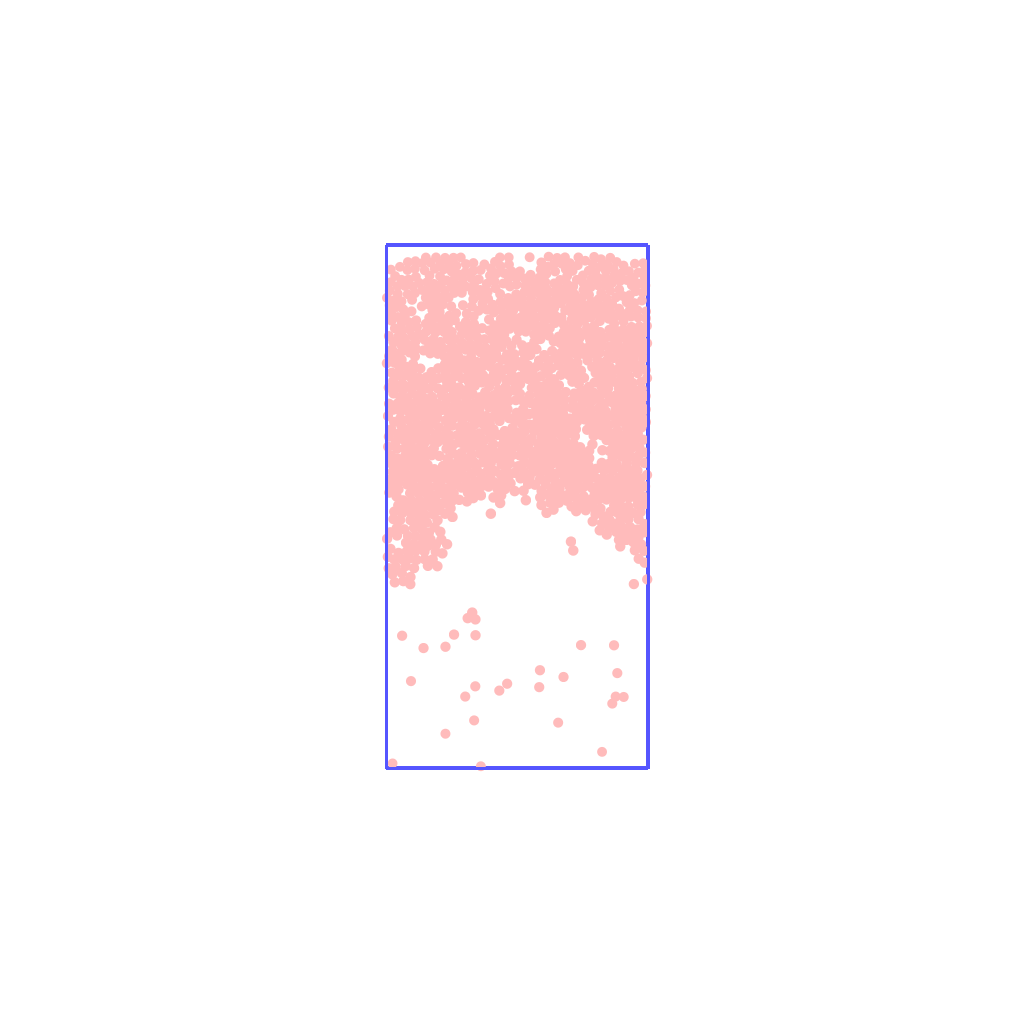
\includegraphics[width=\textwidth]{image/RaRtmap/2023-11-15T10:59:30.665__chi1.265_Ay50_rho0.4_T0.43_dT0.04_Rd0.0_Rt0.375_Ra1.877538_g0.0003999718779659611_run4.0e7_output.png}}
      \subcaption{$\text{R}_\text{a}=1.877,\\\text{R}_\text{t}=0.375$}
      % \label{}
    \end{minipage} \\
    \begin{minipage}[t]{0.2\hsize}
      \centering
      \href{https://youtu.be/S0NOYiYNCBU}{
      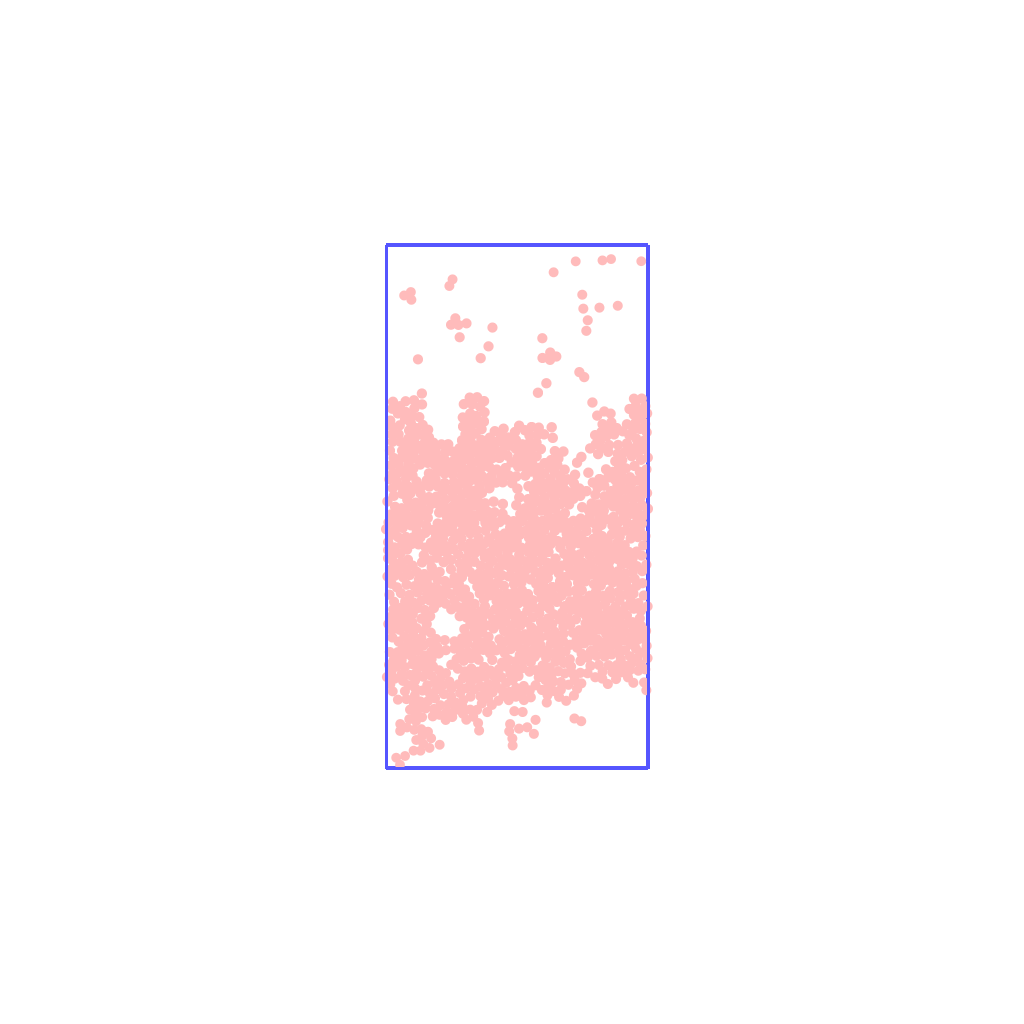
\includegraphics[width=\textwidth]{image/RaRtmap/2023-11-15T11:53:37.697__chi1.265_Ay50_rho0.4_T0.43_dT0.04_Rd0.0_Rt0.5_Ra0.0_g0.0003999718779659611_run4.0e7_output.png}}
      \subcaption{$\text{R}_\text{a}=0.0,\\\text{R}_\text{t}=0.500$}
      % \label{}
    \end{minipage} &
    \begin{minipage}[t]{0.2\hsize}
      \centering
      \href{https://youtu.be/l8Mz0kOFZwY}{
      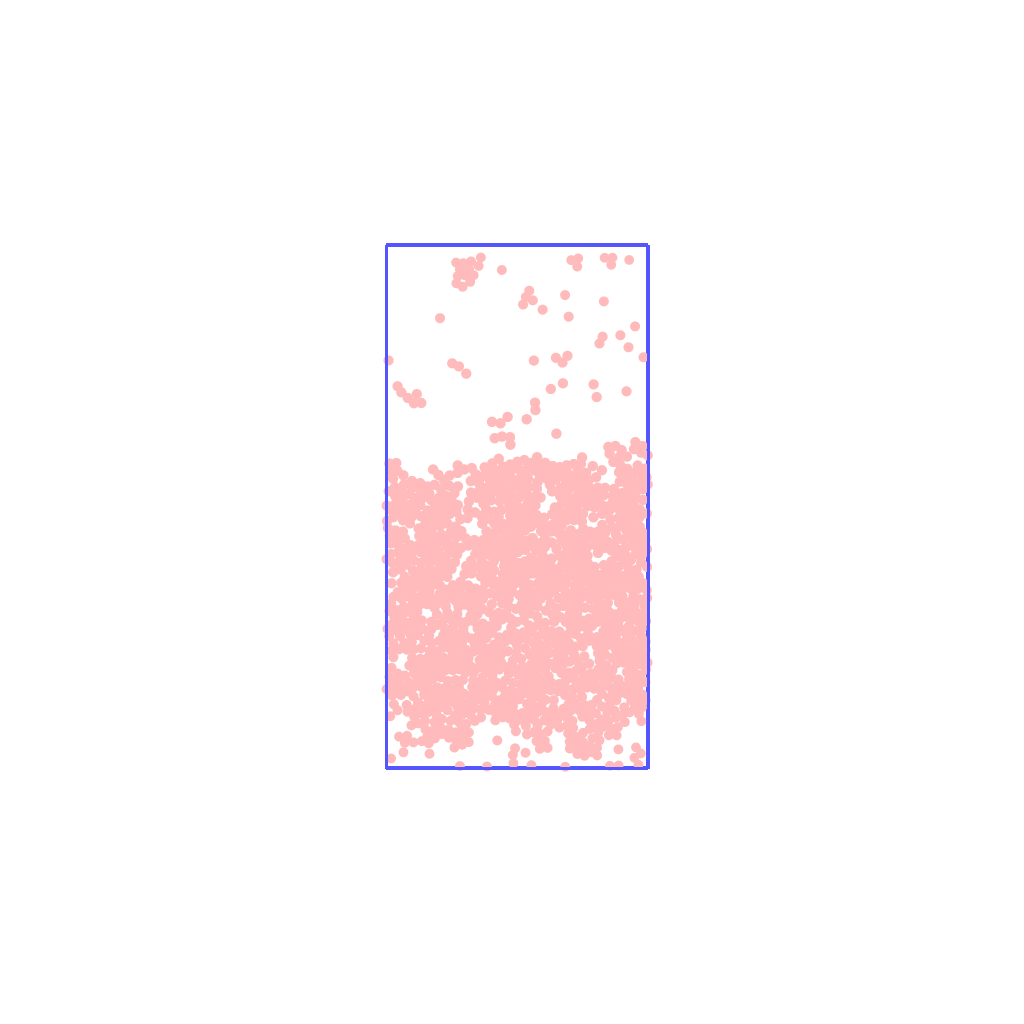
\includegraphics[width=\textwidth]{image/RaRtmap/2023-11-15T12:45:26.303__chi1.265_Ay50_rho0.4_T0.43_dT0.04_Rd0.0_Rt0.5_Ra0.4693845_g0.0003999718779659611_run4.0e7_output.png}}
      \subcaption{$\text{R}_\text{a}=0.469,\\\text{R}_\text{t}=0.500$}
      % \label{}
    \end{minipage} &
    \begin{minipage}[t]{0.2\hsize}
      \centering
      \href{https://youtu.be/pR-P4R70FQg}{
      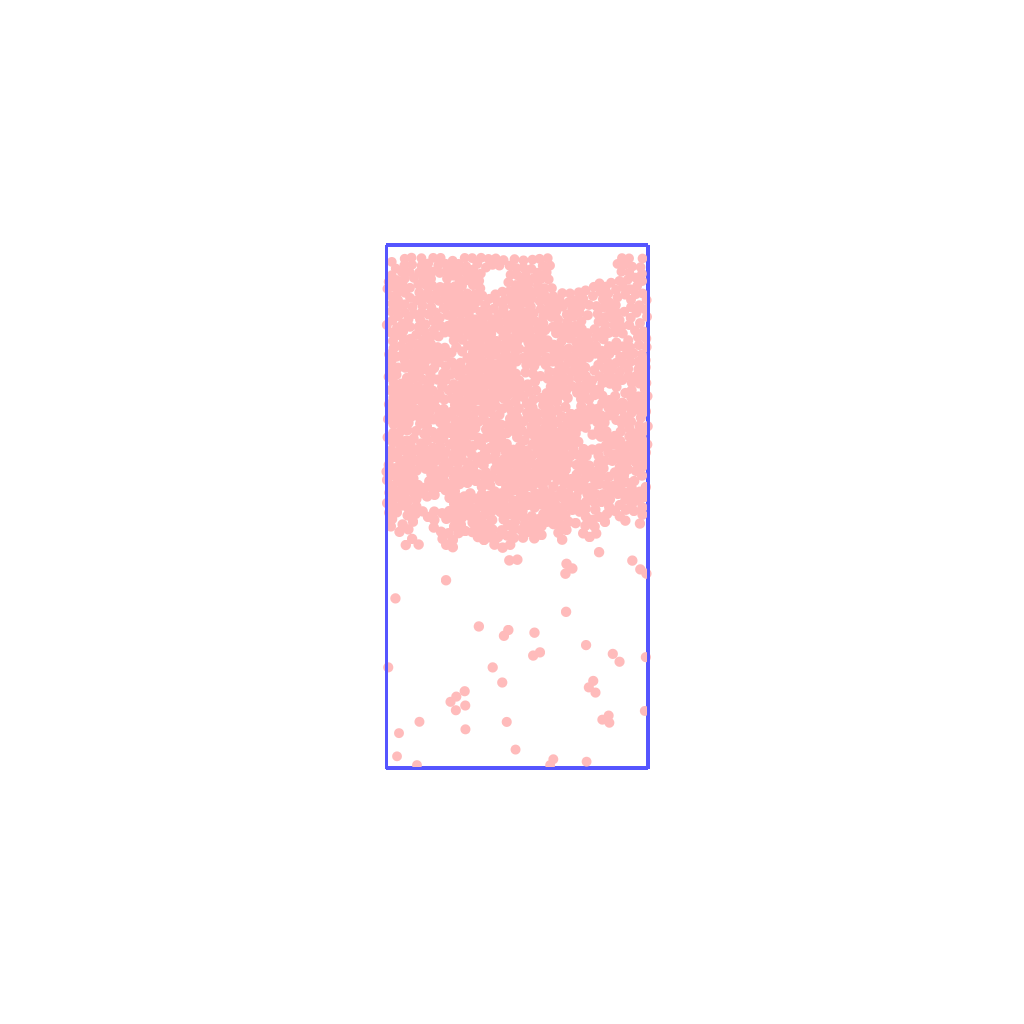
\includegraphics[width=\textwidth]{image/RaRtmap/2023-11-15T13:37:58.058__chi1.265_Ay50_rho0.4_T0.43_dT0.04_Rd0.0_Rt0.5_Ra0.938769_g0.0003999718779659611_run4.0e7_output.png}}
      \subcaption{$\text{R}_\text{a}=0.938,\\\text{R}_\text{t}=0.500$}
      % \label{}
    \end{minipage} &
    \begin{minipage}[t]{0.2\hsize}
      \centering
      \href{https://youtu.be/kSUk1XcKZBA}{
      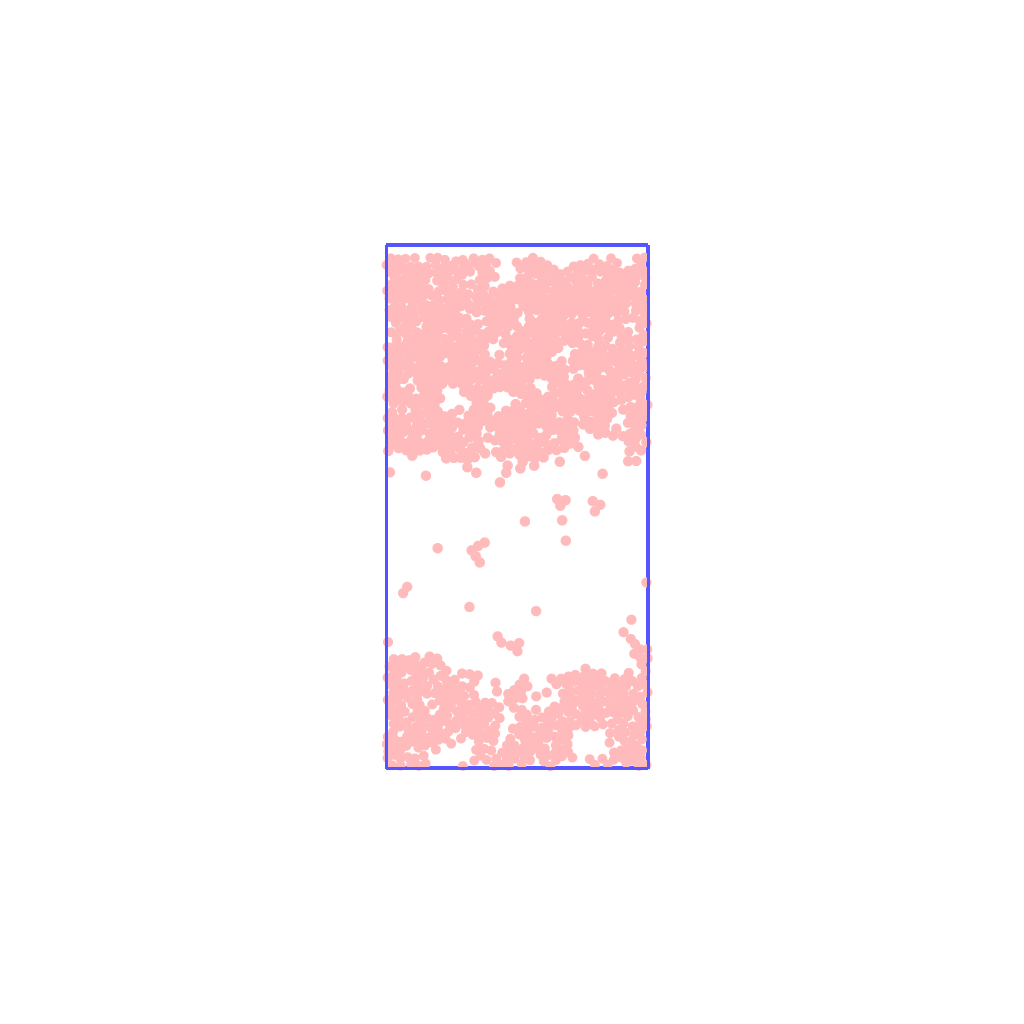
\includegraphics[width=\textwidth]{image/RaRtmap/2023-11-15T14:30:22.529__chi1.265_Ay50_rho0.4_T0.43_dT0.04_Rd0.0_Rt0.5_Ra1.4081535_g0.0003999718779659611_run4.0e7_output.png}}
      \subcaption{$\text{R}_\text{a}=1.408,\\\text{R}_\text{t}=0.500$}
      % \label{}
    \end{minipage} &
    \begin{minipage}[t]{0.2\hsize}
      \centering
      
\includegraphics[width=\textwidth]{image/RaRtmap/2023-11-15T15:21:59.073__chi1.265_Ay50_rho0.4_T0.43_dT0.04_Rd0.0_Rt0.5_Ra1.877538_g0.0003999718779659611_run4.0e7_output.png}
      \subcaption{$\text{R}_\text{a}=1.877,\\\text{R}_\text{t}=0.500$}
      % \label{}
    \end{minipage} 
  \end{tabular}
  \caption{}
  % \lable{}
\end{figure}


重心位置をスケーリングして, 時系列プロットすると,

\begin{figure}[H]
  \begin{tabular}{ccccc}
    \begin{minipage}[t]{0.2\hsize}
      \centering
      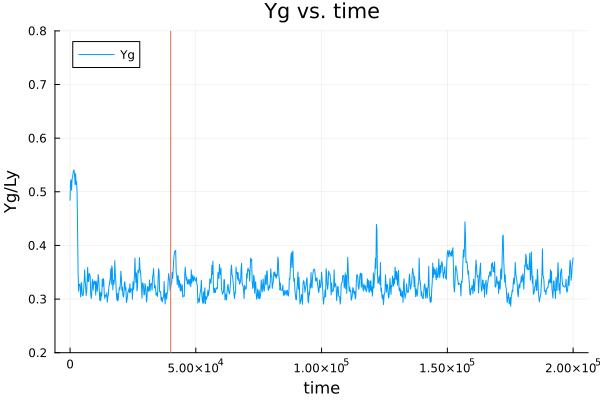
\includegraphics[width=\textwidth]{image/RaRtmap_time/2023-11-14T18:19:29.358__chi1.265_Ay50_rho0.4_T0.43_dT0.04_Rd0.0_Rt0.0_Ra0.0_g0.0003999718779659611_run4.0e7_output.png}
      \subcaption{$\text{R}_\text{a}=0.0,\\\text{R}_\text{t}=0.0$}
      \label{fig:RaRtmap_time_Ra0.0_Rt0.0}
    \end{minipage} &
    \begin{minipage}[t]{0.2\hsize}
      \centering
      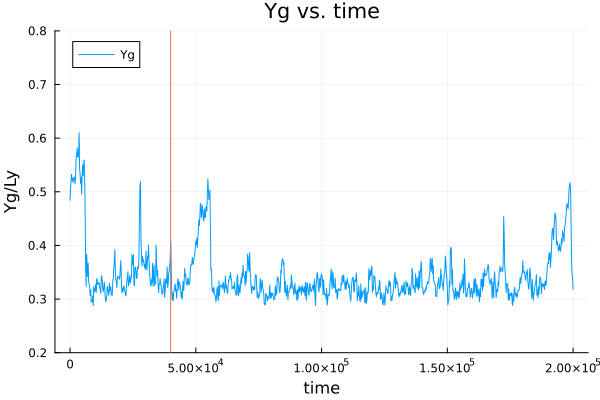
\includegraphics[width=\textwidth]{image/RaRtmap_time/2023-11-14T19:14:52.710__chi1.265_Ay50_rho0.4_T0.43_dT0.04_Rd0.0_Rt0.0_Ra0.4693845_g0.0003999718779659611_run4.0e7_output.png}
      \subcaption{$\text{R}_\text{a}=0.469,\\\text{R}_\text{t}=0.0$}
      \label{}
    \end{minipage} &
    \begin{minipage}[t]{0.2\hsize}
      \centering
      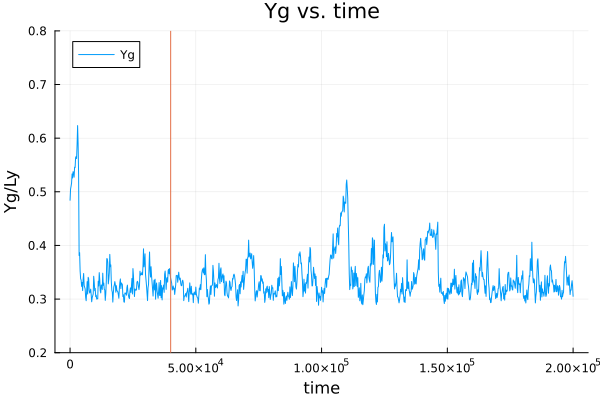
\includegraphics[width=\textwidth]{image/RaRtmap_time/2023-11-14T20:07:58.625__chi1.265_Ay50_rho0.4_T0.43_dT0.04_Rd0.0_Rt0.0_Ra0.938769_g0.0003999718779659611_run4.0e7_output.png}
      \subcaption{$\text{R}_\text{a}=0.938,\\\text{R}_\text{t}=0.0$}
      \label{}
    \end{minipage} &
    \begin{minipage}[t]{0.2\hsize}
      \centering
      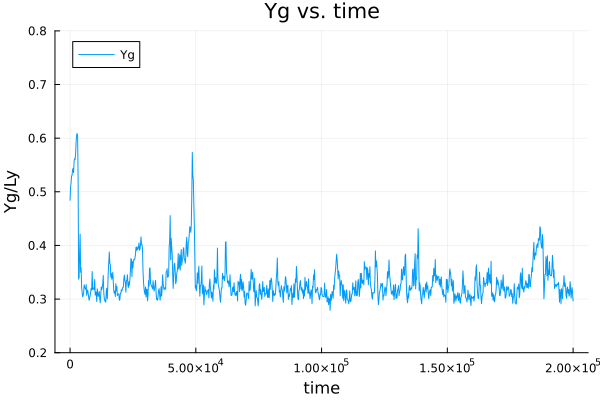
\includegraphics[width=\textwidth]{image/RaRtmap_time/2023-11-14T21:01:09.992__chi1.265_Ay50_rho0.4_T0.43_dT0.04_Rd0.0_Rt0.0_Ra1.4081535_g0.0003999718779659611_run4.0e7_output.png}
      \subcaption{$\text{R}_\text{a}=1.408,\\\text{R}_\text{t}=0.0$}
      \label{}
    \end{minipage} &
    \begin{minipage}[t]{0.2\hsize}
      \centering
      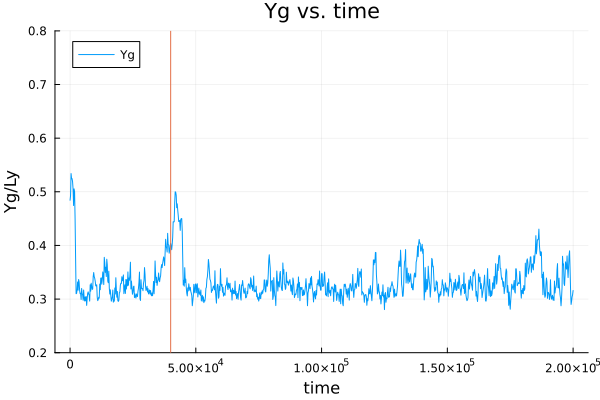
\includegraphics[width=\textwidth]{image/RaRtmap_time/2023-11-14T21:54:59.835__chi1.265_Ay50_rho0.4_T0.43_dT0.04_Rd0.0_Rt0.0_Ra1.877538_g0.0003999718779659611_run4.0e7_output.png}
      \subcaption{$\text{R}_\text{a}=1.877,\\\text{R}_\text{t}=0.0$}
      \label{}
    \end{minipage} \\
    \begin{minipage}[t]{0.2\hsize}
      \centering
      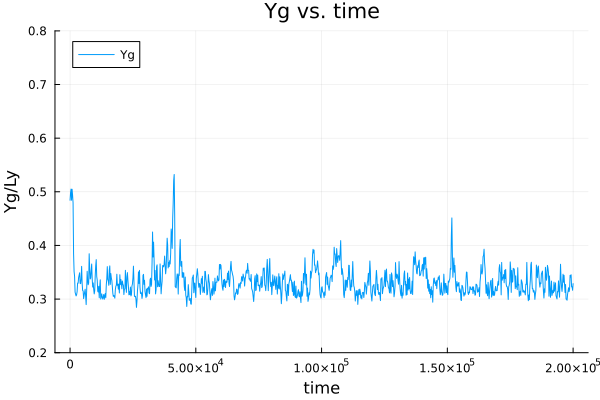
\includegraphics[width=\textwidth]{image/RaRtmap_time/2023-11-14T22:51:24.191__chi1.265_Ay50_rho0.4_T0.43_dT0.04_Rd0.0_Rt0.125_Ra0.0_g0.0003999718779659611_run4.0e7_output.png}
      \subcaption{$\text{R}_\text{a}=0.0,\\\text{R}_\text{t}=0.125$}
      \label{}
    \end{minipage} &
    \begin{minipage}[t]{0.2\hsize}
      \centering
      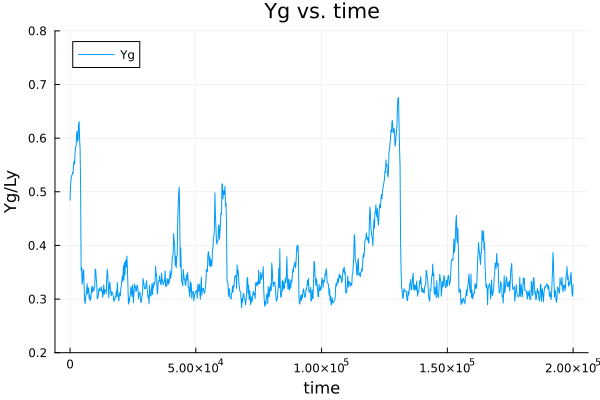
\includegraphics[width=\textwidth]{image/RaRtmap_time/2023-11-14T23:48:31.439__chi1.265_Ay50_rho0.4_T0.43_dT0.04_Rd0.0_Rt0.125_Ra0.4693845_g0.0003999718779659611_run4.0e7_output.png}
      \subcaption{$\text{R}_\text{a}=0.469,\\\text{R}_\text{t}=0.125$}
      \label{}
    \end{minipage} &
    \begin{minipage}[t]{0.2\hsize}
      \centering
      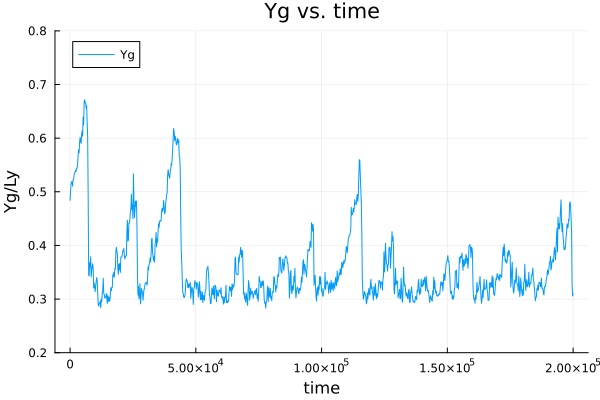
\includegraphics[width=\textwidth]{image/RaRtmap_time/2023-11-15T00:43:33.781__chi1.265_Ay50_rho0.4_T0.43_dT0.04_Rd0.0_Rt0.125_Ra0.938769_g0.0003999718779659611_run4.0e7_output.png}
      \subcaption{$\text{R}_\text{a}=0.938,\\\text{R}_\text{t}=0.125$}
      \label{}
    \end{minipage} &
    \begin{minipage}[t]{0.2\hsize}
      \centering
      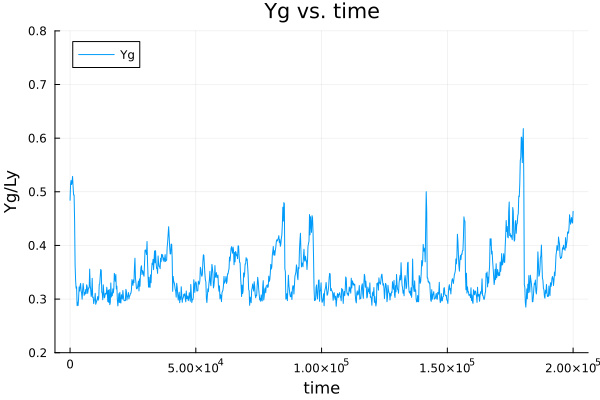
\includegraphics[width=\textwidth]{image/RaRtmap_time/2023-11-15T01:35:17.404__chi1.265_Ay50_rho0.4_T0.43_dT0.04_Rd0.0_Rt0.125_Ra1.4081535_g0.0003999718779659611_run4.0e7_output.png}
      \subcaption{$\text{R}_\text{a}=1.408,\\\text{R}_\text{t}=0.125$}
      \label{}
    \end{minipage} &
    \begin{minipage}[t]{0.2\hsize}
      \centering
      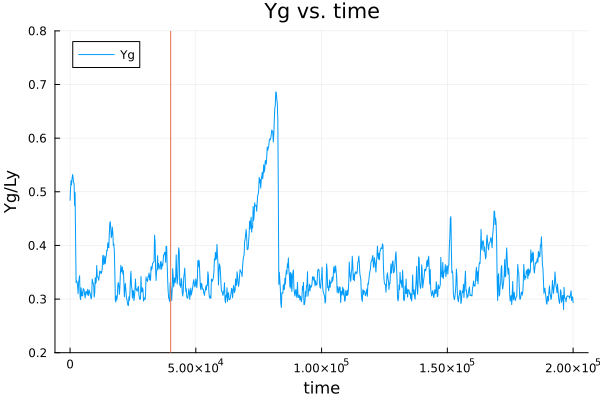
\includegraphics[width=\textwidth]{image/RaRtmap_time/2023-11-15T02:27:34.337__chi1.265_Ay50_rho0.4_T0.43_dT0.04_Rd0.0_Rt0.125_Ra1.877538_g0.0003999718779659611_run4.0e7_output.png}
      \subcaption{$\text{R}_\text{a}=1.877,\\\text{R}_\text{t}=0.125$}
      \label{}
    \end{minipage} \\
    \begin{minipage}[t]{0.2\hsize}
      \centering
      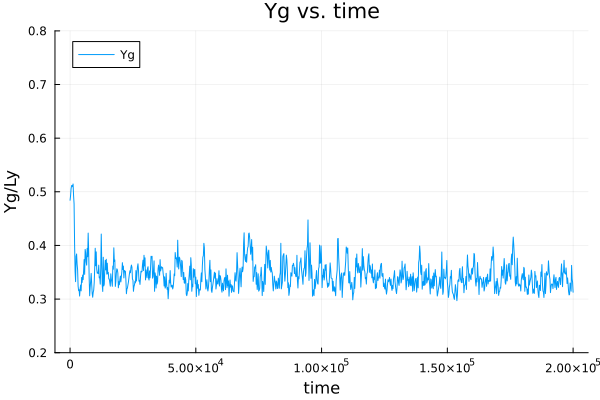
\includegraphics[width=\textwidth]{image/RaRtmap_time/2023-11-15T03:19:32.715__chi1.265_Ay50_rho0.4_T0.43_dT0.04_Rd0.0_Rt0.25_Ra0.0_g0.0003999718779659611_run4.0e7_output.png}
      \subcaption{$\text{R}_\text{a}=0.0,\\\text{R}_\text{t}=0.250$}
      \label{}
    \end{minipage} &
    \begin{minipage}[t]{0.2\hsize}
      \centering
      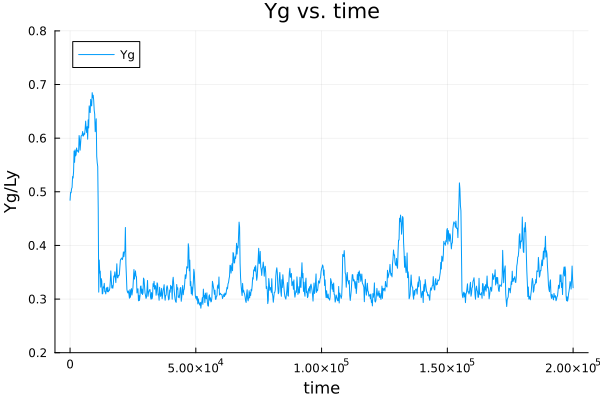
\includegraphics[width=\textwidth]{image/RaRtmap_time/2023-11-15T04:11:00.956__chi1.265_Ay50_rho0.4_T0.43_dT0.04_Rd0.0_Rt0.25_Ra0.4693845_g0.0003999718779659611_run4.0e7_output.png}
      \subcaption{$\text{R}_\text{a}=0.469,\\\text{R}_\text{t}=0.250$}
      \label{}
    \end{minipage} &
    \begin{minipage}[t]{0.2\hsize}
      \centering
      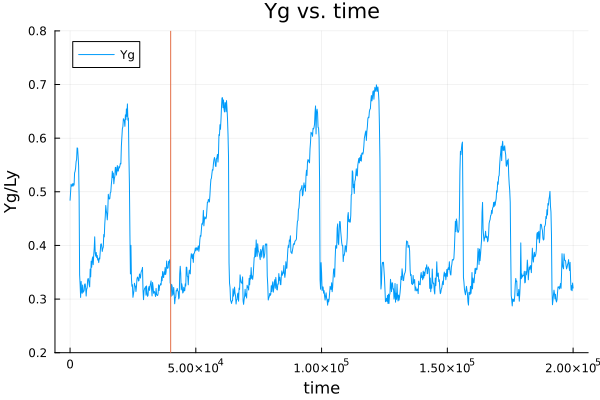
\includegraphics[width=\textwidth]{image/RaRtmap_time/2023-11-15T05:03:45.973__chi1.265_Ay50_rho0.4_T0.43_dT0.04_Rd0.0_Rt0.25_Ra0.938769_g0.0003999718779659611_run4.0e7_output.png}
      \subcaption{$\text{R}_\text{a}=0.938,\\\text{R}_\text{t}=0.250$}
      \label{}
    \end{minipage} &
    \begin{minipage}[t]{0.2\hsize}
      \centering
      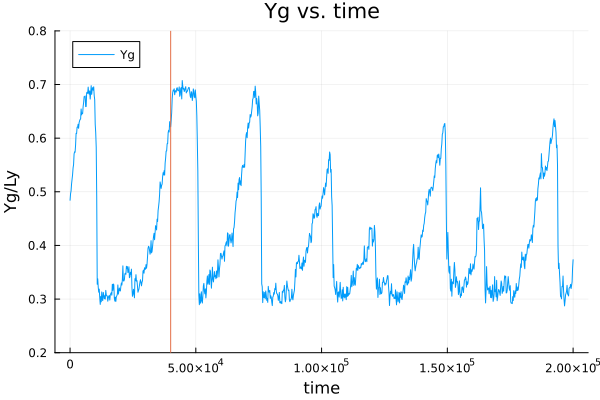
\includegraphics[width=\textwidth]{image/RaRtmap_time/2023-11-15T05:53:00.667__chi1.265_Ay50_rho0.4_T0.43_dT0.04_Rd0.0_Rt0.25_Ra1.4081535_g0.0003999718779659611_run4.0e7_output.png}
      \subcaption{$\text{R}_\text{a}=1.408,\\\text{R}_\text{t}=0.250$}
      \label{}
    \end{minipage} &
    \begin{minipage}[t]{0.2\hsize}
      \centering
      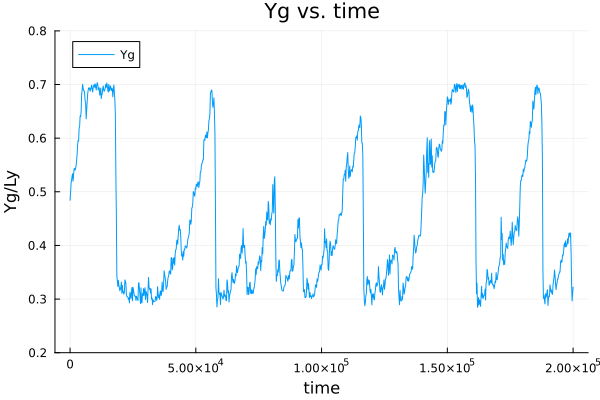
\includegraphics[width=\textwidth]{image/RaRtmap_time/2023-11-15T06:43:21.554__chi1.265_Ay50_rho0.4_T0.43_dT0.04_Rd0.0_Rt0.25_Ra1.877538_g0.0003999718779659611_run4.0e7_output.png}
      \subcaption{$\text{R}_\text{a}=1.877,\\\text{R}_\text{t}=0.250$}
      \label{}
    \end{minipage} \\
    \begin{minipage}[t]{0.2\hsize}
      \centering
      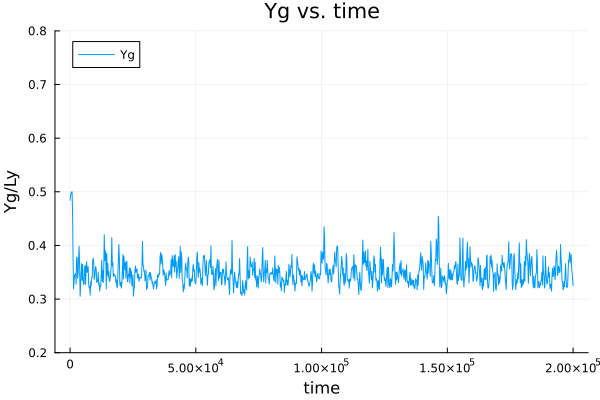
\includegraphics[width=\textwidth]{image/RaRtmap_time/2023-11-15T07:34:00.555__chi1.265_Ay50_rho0.4_T0.43_dT0.04_Rd0.0_Rt0.375_Ra0.0_g0.0003999718779659611_run4.0e7_output.png}
      \subcaption{$\text{R}_\text{a}=0.0,\\\text{R}_\text{t}=0.375$}
      \label{}
    \end{minipage} &
    \begin{minipage}[t]{0.2\hsize}
      \centering
      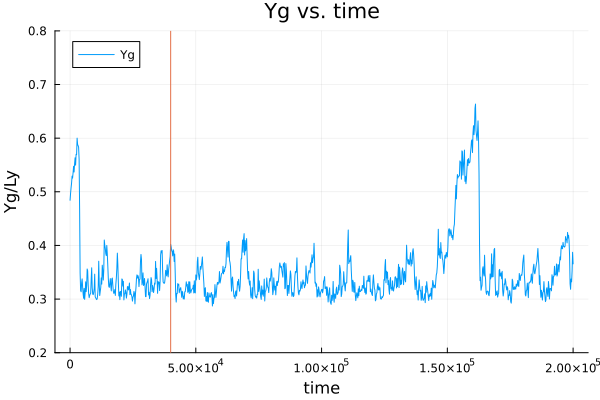
\includegraphics[width=\textwidth]{image/RaRtmap_time/2023-11-15T08:24:37.362__chi1.265_Ay50_rho0.4_T0.43_dT0.04_Rd0.0_Rt0.375_Ra0.4693845_g0.0003999718779659611_run4.0e7_output.png}
      \subcaption{$\text{R}_\text{a}=0.469,\\\text{R}_\text{t}=0.375$}
      \label{}
    \end{minipage} &
    \begin{minipage}[t]{0.2\hsize}
      \centering
      \includegraphics[width=\textwidth]{image/RaRtmap_time/2023-11-15T09:16:40.082__chi1.265_Ay50_rho0.4_T0.43_dT0.04_Rd0.0_Rt0.375_Ra0.938769_g0.0003999718779659611_run4.0e7_output.png}
      \subcaption{$\text{R}_\text{a}=0.938,\\\text{R}_\text{t}=0.375$}
      \label{}
    \end{minipage} &
    \begin{minipage}[t]{0.2\hsize}
      \centering
      \includegraphics[width=\textwidth]{image/RaRtmap_time/2023-11-15T10:07:20.945__chi1.265_Ay50_rho0.4_T0.43_dT0.04_Rd0.0_Rt0.375_Ra1.4081535_g0.0003999718779659611_run4.0e7_output.png}
      \subcaption{$\text{R}_\text{a}=1.408,\\\text{R}_\text{t}=0.375$}
      \label{}
    \end{minipage} &
    \begin{minipage}[t]{0.2\hsize}
      \centering
      \includegraphics[width=\textwidth]{image/RaRtmap_time/2023-11-15T10:59:30.665__chi1.265_Ay50_rho0.4_T0.43_dT0.04_Rd0.0_Rt0.375_Ra1.877538_g0.0003999718779659611_run4.0e7_output.png}
      \subcaption{$\text{R}_\text{a}=1.877,\\\text{R}_\text{t}=0.375$}
      \label{}
    \end{minipage} \\
    \begin{minipage}[t]{0.2\hsize}
      \centering
      \includegraphics[width=\textwidth]{image/RaRtmap_time/2023-11-15T11:53:37.697__chi1.265_Ay50_rho0.4_T0.43_dT0.04_Rd0.0_Rt0.5_Ra0.0_g0.0003999718779659611_run4.0e7_output.png}
      \subcaption{$\text{R}_\text{a}=0.0,\\\text{R}_\text{t}=0.500$}
      \label{}
    \end{minipage} &
    \begin{minipage}[t]{0.2\hsize}
      \centering
      \includegraphics[width=\textwidth]{image/RaRtmap_time/2023-11-15T12:45:26.303__chi1.265_Ay50_rho0.4_T0.43_dT0.04_Rd0.0_Rt0.5_Ra0.4693845_g0.0003999718779659611_run4.0e7_output.png}
      \subcaption{$\text{R}_\text{a}=0.469,\\\text{R}_\text{t}=0.500$}
      \label{fig:RaRtmap_time_Ra0.469_Rt0.500}
    \end{minipage} &
    \begin{minipage}[t]{0.2\hsize}
      \centering
      \includegraphics[width=\textwidth]{image/RaRtmap_time/2023-11-15T13:37:58.058__chi1.265_Ay50_rho0.4_T0.43_dT0.04_Rd0.0_Rt0.5_Ra0.938769_g0.0003999718779659611_run4.0e7_output.png}
      \subcaption{$\text{R}_\text{a}=0.938,\\\text{R}_\text{t}=0.500$}
      \label{fig:RaRtmap_time_Ra0.938_Rt0.500}
    \end{minipage} &
    \begin{minipage}[t]{0.2\hsize}
      \centering
      \includegraphics[width=\textwidth]{image/RaRtmap_time/2023-11-15T14:30:22.529__chi1.265_Ay50_rho0.4_T0.43_dT0.04_Rd0.0_Rt0.5_Ra1.4081535_g0.0003999718779659611_run4.0e7_output.png}
      \subcaption{$\text{R}_\text{a}=1.408,\\\text{R}_\text{t}=0.500$}
      \label{}
    \end{minipage} &
    \begin{minipage}[t]{0.2\hsize}
      \centering
      \includegraphics[width=\textwidth]{image/RaRtmap_time/2023-11-15T15:21:59.073__chi1.265_Ay50_rho0.4_T0.43_dT0.04_Rd0.0_Rt0.5_Ra1.877538_g0.0003999718779659611_run4.0e7_output.png}
      \subcaption{$\text{R}_\text{a}=1.877,\\\text{R}_\text{t}=0.500$}
      \label{}
    \end{minipage} 
  \end{tabular}
  \caption{$t_i = 0, t_f = 2.0 \times 10^5, \dd t \sqrt{\varepsilon / m \sigma^2}= 0.005, t \sqrt{\varepsilon / m \sigma^2} = 200 ごとにプロット.$}
  \label{fig:RaRtmap_time}
\end{figure}


重心位置の揺らぎについて同時プロットで表してみる. 図\ref{fig:RaRtmap_time_Ra0.0_Rt0.0}から$\tau \sqrt{\varepsilon / m \sigma^2} = 2.5 \times 10^{4}$からのデータを用いてプロットしている.

\begin{figure}[H]
  \begin{tabular}{cc}
    \begin{minipage}[t]{0.5\hsize}
      \centering
      \includegraphics[width=\textwidth]{image/lnStdYg_Ra_ti25000.png}
      \subcaption{}
      \label{}
    \end{minipage}
    \begin{minipage}[t]{0.5\hsize}
      \centering
      \includegraphics[width=\textwidth]{image/lnStdYg_Rt_ti25000.png}
      \subcaption{}
      \label{}
    \end{minipage}
  \end{tabular}
  \caption{}
  \label{}
\end{figure}

\subsection{周期性}

重心位置が周期的に変化しているのかを調べたい.

図\ref{fig:RaRtmap_time_Ra0.469_Rt0.500}と図\ref{fig:RaRtmap_time_Ra0.938_Rt0.500}の間をもっと詳しく見る.



% \section{分析}

この章では, \ref{sec:simulation}章において行ったシミュレーションに対して, それぞれ分析をしていく.

\subsection{$\text{R}_\text{a}$, $\text{R}_\text{t}$ マップ}


ここで, 重心の標準偏差は以下のように書くことができる.

\begin{align}
  \sigma (Y_g) &= \sqrt{\frac{1}{N_{D}}\sum_{t=t_i}^{t=t_f} (Y_{g}(t) - \bar{Y_g})^2}
\end{align}

重心位置の標準偏差について同時プロットで表してみる. 以降の解析は図\ref{fig:RaRtmap_time_Ra0.0_Rt0.0}から定常状態にあるとみなせる, $t_i \sqrt{\varepsilon / m \sigma^2} = 2.5 \times 10^{4}$からのデータを用いてプロットすることにしている.

\begin{figure}[H]
  \begin{tabular}{cc}
    \begin{minipage}[t]{0.5\hsize}
      \centering
      \includegraphics[width=\textwidth]{image/lnStdYg_Ra0.0to1.877538_Rt0.0to0.5_ti25000.png}
      \subcaption{}
      \label{}
    \end{minipage}
    \begin{minipage}[t]{0.5\hsize}
      \centering
      \includegraphics[width=\textwidth]{image/lnStdYg_Rt0.0to0.5_Ra0.0to1.877538_ti25000.png}
      \subcaption{}
      \label{}
    \end{minipage}
  \end{tabular}
  \caption{$t_i \sqrt{\varepsilon / m \sigma^2} = 2.5 \times 10^{4}$}
  \label{}
\end{figure}

\subsection{周期性}

重心位置が周期的に変化しているのかを調べたい.

図\ref{fig:RaRtmap_time_Ra0.469_Rt0.500}$R_a = 0.469, R_t = 0.5$と図\ref{fig:RaRtmap_time_Ra0.938_Rt0.500} $R_a = 0.938, R_t = 0.5$の間をもっと詳しく見る.

\begin{figure}[H]
  \centering
  \begin{tabular}{ccccc}
    \begin{minipage}[t]{0.2\hsize}
      \centering
      \includegraphics[width=\textwidth]{image/RaRtmap_time/2023-11-22T18:19:26.970_RaRt_chi1.265_Ay50_rho0.4_T0.43_dT0.04_Rd0.0_Rt0.5_Ra0.4693845_g0.0003999718779659611_run1.2e8.png}
      \subcaption{Ra0.4693845}
      \label{}
    \end{minipage} &
    \begin{minipage}[t]{0.2\hsize}
      \centering
      \includegraphics[width=\textwidth]{image/RaRtmap_time/2023-11-22T18:19:27.571_RaRt_chi1.265_Ay50_rho0.4_T0.43_dT0.04_Rd0.0_Rt0.5_Ra0.586730625_g0.0003999718779659611_run1.2e8.png}
      \subcaption{Ra0.586730625}
      \label{}
    \end{minipage} &
    \begin{minipage}[t]{0.2\hsize}
      \centering
      \includegraphics[width=\textwidth]{image/RaRtmap_time/2023-11-22T18:19:27.653_RaRt_chi1.265_Ay50_rho0.4_T0.43_dT0.04_Rd0.0_Rt0.5_Ra0.70407675_g0.0003999718779659611_run1.2e8.png}
      \subcaption{Ra0.70407675}
      \label{}
    \end{minipage} &
    \begin{minipage}[t]{0.2\hsize}
      \centering
      \includegraphics[width=\textwidth]{image/RaRtmap_time/2023-11-22T18:19:27.720_RaRt_chi1.265_Ay50_rho0.4_T0.43_dT0.04_Rd0.0_Rt0.5_Ra0.821422875_g0.0003999718779659611_run1.2e8.png}
      \subcaption{Ra0.821422875}
      \label{}
    \end{minipage} &
    \begin{minipage}[t]{0.2\hsize}
      \centering
      \includegraphics[width=\textwidth]{image/RaRtmap_time/2023-11-22T18:19:27.787_RaRt_chi1.265_Ay50_rho0.4_T0.43_dT0.04_Rd0.0_Rt0.5_Ra0.938769_g0.0003999718779659611_run1.2e8.png}
      \subcaption{Ra0.938769}
      \label{}
    \end{minipage} 
  \end{tabular}
  \caption{}
  \label{}
\end{figure}

\begin{figure}[H]
  \centering
  \includegraphics[scale=0.5]{image/lnStdYg_Ra0.4693845to0.98769_Rt0.5_ti25000.png}
  \caption{}
  \label{}
\end{figure}

% \begin{figure}[H]
%   \centering
%   \includegraphics[scale=0.6]{image/RaRtmap_time/2023-11-27T01:34:51.948_Ra_chi1.265_Ay50_rho0.4_T0.43_dT0.04_Rd0.0_Rt0.5_Ra0.70407675_g0.0003999718779659611_run1.2e9.png}
%   \caption{Ra0.4693845}
%   \label{}
% \end{figure}

\begin{figure}[H]
  \centering
  \begin{tabular}{ccccc}
    \begin{minipage}[t]{0.2\hsize}
      \centering
      \includegraphics[width=\textwidth]{image/RaRtmap_time/2023-11-27T01:34:51.948_Ra_chi1.265_Ay50_rho0.4_T0.43_dT0.04_Rd0.0_Rt0.5_Ra0.70407675_g0.0003999718779659611_run1.2e9.png}
      \subcaption{Ra0.70407675}
      \label{}
    \end{minipage} &
    \begin{minipage}[t]{0.2\hsize}
      \centering
      \includegraphics[width=\textwidth]{image/RaRtmap_time/2023-11-27T01:34:52.442_Ra_chi1.265_Ay50_rho0.4_T0.43_dT0.04_Rd0.0_Rt0.5_Ra0.7627498125_g0.0003999718779659611_run1.2e9.png}
      \subcaption{Ra0.7627498125}
      \label{}
    \end{minipage} &
    \begin{minipage}[t]{0.2\hsize}
      \centering
      \includegraphics[width=\textwidth]{image/RaRtmap_time/2023-11-27T01:34:52.545_Ra_chi1.265_Ay50_rho0.4_T0.43_dT0.04_Rd0.0_Rt0.5_Ra0.821422875_g0.0003999718779659611_run1.2e9.png}
      \subcaption{Ra0.821422875}
      \label{}
    \end{minipage} &
    \begin{minipage}[t]{0.2\hsize}
      \centering
      \includegraphics[width=\textwidth]{image/RaRtmap_time/2023-11-27T01:34:52.610_Ra_chi1.265_Ay50_rho0.4_T0.43_dT0.04_Rd0.0_Rt0.5_Ra0.8800959375_g0.0003999718779659611_run1.2e9.png}
      \subcaption{Ra0.8800959375}
      \label{}
    \end{minipage} &
    \begin{minipage}[t]{0.2\hsize}
      \centering
      \includegraphics[width=\textwidth]{image/RaRtmap_time/2023-11-27T01:34:52.675_Ra_chi1.265_Ay50_rho0.4_T0.43_dT0.04_Rd0.0_Rt0.5_Ra0.938769_g0.0003999718779659611_run1.2e9.png}
      \subcaption{Ra0.938769}
      \label{}
    \end{minipage} 
  \end{tabular}
  \caption{$t_i = 0 , t_f = 6.0 \times 10^6, t\sqrt{\epsilon/m{\sigma}^2} = 6000$ごとにプロット.}
  \label{}
\end{figure}

\begin{figure}[H]
  \centering
  \includegraphics[scale=0.5]{image/lnStdYg_Ra0.70407675to0.98769_Rt0.5_ti25000.png}
  \caption{}
  \label{}
\end{figure}

図\ref{fig:RaRtmap_time_Ra0.469_Rt0.500}$R_a = 0.469, R_t = 0.5$と図\ref{fig:RaRtmap_time_Ra0.938_Rt0.500} $R_a = 0.938, R_t = 0.5$の間をもっと詳しく見る. その際, 簡単のため, $Ra =0.5 \sim 1.0$の間を見ることにする.

\begin{figure}[H]
  \centering
  \begin{tabular}{ccccc}
    \begin{minipage}[t]{0.2\hsize}
      \centering
      \includegraphics[width=\textwidth]{image/RaRtmap_time/2023-11-30T20:13:31.872_Ra_chi1.265_Ay50_rho0.4_T0.43_dT0.04_Rd0.0_Rt0.5_Ra0.5_g0.0003999718779659611_run1.2e9.png}
      \subcaption{Ra0.5}
      \label{}
    \end{minipage} &
    \begin{minipage}[t]{0.2\hsize}
      \centering
      \includegraphics[width=\textwidth]{image/RaRtmap_time/2023-11-30T20:13:32.405_Ra_chi1.265_Ay50_rho0.4_T0.43_dT0.04_Rd0.0_Rt0.5_Ra0.625_g0.0003999718779659611_run1.2e9.png}
      \subcaption{Ra0.625}
      \label{}
    \end{minipage} &
    \begin{minipage}[t]{0.2\hsize}
      \centering
      \includegraphics[width=\textwidth]{image/RaRtmap_time/2023-11-30T20:13:32.471_Ra_chi1.265_Ay50_rho0.4_T0.43_dT0.04_Rd0.0_Rt0.5_Ra0.75_g0.0003999718779659611_run1.2e9.png}
      \subcaption{Ra0.75}
      \label{}
    \end{minipage} &
    \begin{minipage}[t]{0.2\hsize}
      \centering
      \includegraphics[width=\textwidth]{image/RaRtmap_time/2023-11-30T20:13:32.545_Ra_chi1.265_Ay50_rho0.4_T0.43_dT0.04_Rd0.0_Rt0.5_Ra0.875_g0.0003999718779659611_run1.2e9.png}
      \subcaption{Ra0.875}
      \label{}
    \end{minipage} &
    \begin{minipage}[t]{0.2\hsize}
      \centering
      \includegraphics[width=\textwidth]{image/RaRtmap_time/2023-11-30T20:13:32.620_Ra_chi1.265_Ay50_rho0.4_T0.43_dT0.04_Rd0.0_Rt0.5_Ra1.0_g0.0003999718779659611_run1.2e9.png}
      \subcaption{Ra1.0}
      \label{}
    \end{minipage} 
  \end{tabular}
  \caption{}
  \label{}
\end{figure}

\begin{figure}[H]
  \centering
  \includegraphics[scale=0.5]{image/lnStdYg_Ra0.5to1.0_Rt0.5_ti25000.png}
  \caption{}
  \label{}
\end{figure}


\subsection{ヒストグラム}

\subsubsection{重力と熱流を同時にかける}

図\ref{fig:RaRtmap_time}の結果をそれぞれ正規化したヒストグラムにして表す.

\begin{figure}[H]
  \begin{tabular}{ccccc}
    \begin{minipage}[t]{0.2\hsize}
      \centering
      \includegraphics[width=\textwidth]{image/RaRtmap_hist/2023-11-14T18:19:29.358__chi1.265_Ay50_rho0.4_T0.43_dT0.04_Rd0.0_Rt0.0_Ra0.0_g0.0003999718779659611_run4.0e7_output.png}
      \subcaption{$\text{R}_\text{a}=0.0,\text{R}_\text{t}=0.0$}
      \label{fig:RaRtmap_hist_Ra0.0_Rt0.0}
    \end{minipage} &
    \begin{minipage}[t]{0.2\hsize}
      \centering
      \includegraphics[width=\textwidth]{image/RaRtmap_hist/2023-11-14T19:14:52.710__chi1.265_Ay50_rho0.4_T0.43_dT0.04_Rd0.0_Rt0.0_Ra0.4693845_g0.0003999718779659611_run4.0e7_output.png}
      \subcaption{$\text{R}_\text{a}=0.469,\\\text{R}_\text{t}=0.0$}
      \label{}
    \end{minipage} &
    \begin{minipage}[t]{0.2\hsize}
      \centering
      \includegraphics[width=\textwidth]{image/RaRtmap_hist/2023-11-14T20:07:58.625__chi1.265_Ay50_rho0.4_T0.43_dT0.04_Rd0.0_Rt0.0_Ra0.938769_g0.0003999718779659611_run4.0e7_output.png}
      \subcaption{$\text{R}_\text{a}=0.938,\\\text{R}_\text{t}=0.0$}
      \label{}
    \end{minipage} &
    \begin{minipage}[t]{0.2\hsize}
      \centering
      \includegraphics[width=\textwidth]{image/RaRtmap_hist/2023-11-14T21:01:09.992__chi1.265_Ay50_rho0.4_T0.43_dT0.04_Rd0.0_Rt0.0_Ra1.4081535_g0.0003999718779659611_run4.0e7_output.png}
      \subcaption{$\text{R}_\text{a}=1.408,\\\text{R}_\text{t}=0.0$}
      \label{}
    \end{minipage} &
    \begin{minipage}[t]{0.2\hsize}
      \centering
      \includegraphics[width=\textwidth]{image/RaRtmap_hist/2023-11-14T21:54:59.835__chi1.265_Ay50_rho0.4_T0.43_dT0.04_Rd0.0_Rt0.0_Ra1.877538_g0.0003999718779659611_run4.0e7_output.png}
      \subcaption{$\text{R}_\text{a}=1.877,\\\text{R}_\text{t}=0.0$}
      \label{}
    \end{minipage} \\
    \begin{minipage}[t]{0.2\hsize}
      \centering
      \includegraphics[width=\textwidth]{image/RaRtmap_hist/2023-11-14T22:51:24.191__chi1.265_Ay50_rho0.4_T0.43_dT0.04_Rd0.0_Rt0.125_Ra0.0_g0.0003999718779659611_run4.0e7_output.png}
      \subcaption{$\text{R}_\text{a}=0.0,\\\text{R}_\text{t}=0.125$}
      \label{}
    \end{minipage} &
    \begin{minipage}[t]{0.2\hsize}
      \centering
      \includegraphics[width=\textwidth]{image/RaRtmap_hist/2023-11-14T23:48:31.439__chi1.265_Ay50_rho0.4_T0.43_dT0.04_Rd0.0_Rt0.125_Ra0.4693845_g0.0003999718779659611_run4.0e7_output.png}
      \subcaption{$\text{R}_\text{a}=0.469,\\\text{R}_\text{t}=0.125$}
      \label{}
    \end{minipage} &
    \begin{minipage}[t]{0.2\hsize}
      \centering
      \includegraphics[width=\textwidth]{image/RaRtmap_hist/2023-11-15T00:43:33.781__chi1.265_Ay50_rho0.4_T0.43_dT0.04_Rd0.0_Rt0.125_Ra0.938769_g0.0003999718779659611_run4.0e7_output.png}
      \subcaption{$\text{R}_\text{a}=0.938,\\\text{R}_\text{t}=0.125$}
      \label{}
    \end{minipage} &
    \begin{minipage}[t]{0.2\hsize}
      \centering
      \includegraphics[width=\textwidth]{image/RaRtmap_hist/2023-11-15T01:35:17.404__chi1.265_Ay50_rho0.4_T0.43_dT0.04_Rd0.0_Rt0.125_Ra1.4081535_g0.0003999718779659611_run4.0e7_output.png}
      \subcaption{$\text{R}_\text{a}=1.408,\\\text{R}_\text{t}=0.125$}
      \label{}
    \end{minipage} &
    \begin{minipage}[t]{0.2\hsize}
      \centering
      \includegraphics[width=\textwidth]{image/RaRtmap_hist/2023-11-15T02:27:34.337__chi1.265_Ay50_rho0.4_T0.43_dT0.04_Rd0.0_Rt0.125_Ra1.877538_g0.0003999718779659611_run4.0e7_output.png}
      \subcaption{$\text{R}_\text{a}=1.877,\\\text{R}_\text{t}=0.125$}
      \label{}
    \end{minipage} \\
    \begin{minipage}[t]{0.2\hsize}
      \centering
      \includegraphics[width=\textwidth]{image/RaRtmap_hist/2023-11-15T03:19:32.715__chi1.265_Ay50_rho0.4_T0.43_dT0.04_Rd0.0_Rt0.25_Ra0.0_g0.0003999718779659611_run4.0e7_output.png}
      \subcaption{$\text{R}_\text{a}=0.0,\\\text{R}_\text{t}=0.250$}
      \label{}
    \end{minipage} &
    \begin{minipage}[t]{0.2\hsize}
      \centering
      \includegraphics[width=\textwidth]{image/RaRtmap_hist/2023-11-15T04:11:00.956__chi1.265_Ay50_rho0.4_T0.43_dT0.04_Rd0.0_Rt0.25_Ra0.4693845_g0.0003999718779659611_run4.0e7_output.png}
      \subcaption{$\text{R}_\text{a}=0.469,\\\text{R}_\text{t}=0.250$}
      \label{}
    \end{minipage} &
    \begin{minipage}[t]{0.2\hsize}
      \centering
      \includegraphics[width=\textwidth]{image/RaRtmap_hist/2023-11-15T05:03:45.973__chi1.265_Ay50_rho0.4_T0.43_dT0.04_Rd0.0_Rt0.25_Ra0.938769_g0.0003999718779659611_run4.0e7_output.png}
      \subcaption{$\text{R}_\text{a}=0.938,\\\text{R}_\text{t}=0.250$}
      \label{}
    \end{minipage} &
    \begin{minipage}[t]{0.2\hsize}
      \centering
      \includegraphics[width=\textwidth]{image/RaRtmap_hist/2023-11-15T05:53:00.667__chi1.265_Ay50_rho0.4_T0.43_dT0.04_Rd0.0_Rt0.25_Ra1.4081535_g0.0003999718779659611_run4.0e7_output.png}
      \subcaption{$\text{R}_\text{a}=1.408,\\\text{R}_\text{t}=0.250$}
      \label{}
    \end{minipage} &
    \begin{minipage}[t]{0.2\hsize}
      \centering
      \includegraphics[width=\textwidth]{image/RaRtmap_hist/2023-11-15T06:43:21.554__chi1.265_Ay50_rho0.4_T0.43_dT0.04_Rd0.0_Rt0.25_Ra1.877538_g0.0003999718779659611_run4.0e7_output.png}
      \subcaption{$\text{R}_\text{a}=1.877,\\\text{R}_\text{t}=0.250$}
      \label{}
    \end{minipage} \\
    \begin{minipage}[t]{0.2\hsize}
      \centering
      \includegraphics[width=\textwidth]{image/RaRtmap_hist/2023-11-15T07:34:00.555__chi1.265_Ay50_rho0.4_T0.43_dT0.04_Rd0.0_Rt0.375_Ra0.0_g0.0003999718779659611_run4.0e7_output.png}
      \subcaption{$\text{R}_\text{a}=0.0,\\\text{R}_\text{t}=0.375$}
      \label{}
    \end{minipage} &
    \begin{minipage}[t]{0.2\hsize}
      \centering
      \includegraphics[width=\textwidth]{image/RaRtmap_hist/2023-11-15T08:24:37.362__chi1.265_Ay50_rho0.4_T0.43_dT0.04_Rd0.0_Rt0.375_Ra0.4693845_g0.0003999718779659611_run4.0e7_output.png}
      \subcaption{$\text{R}_\text{a}=0.469,\\\text{R}_\text{t}=0.375$}
      \label{}
    \end{minipage} &
    \begin{minipage}[t]{0.2\hsize}
      \centering
      \includegraphics[width=\textwidth]{image/RaRtmap_hist/2023-11-15T09:16:40.082__chi1.265_Ay50_rho0.4_T0.43_dT0.04_Rd0.0_Rt0.375_Ra0.938769_g0.0003999718779659611_run4.0e7_output.png}
      \subcaption{$\text{R}_\text{a}=0.938,\\\text{R}_\text{t}=0.375$}
      \label{}
    \end{minipage} &
    \begin{minipage}[t]{0.2\hsize}
      \centering
      \includegraphics[width=\textwidth]{image/RaRtmap_hist/2023-11-15T10:07:20.945__chi1.265_Ay50_rho0.4_T0.43_dT0.04_Rd0.0_Rt0.375_Ra1.4081535_g0.0003999718779659611_run4.0e7_output.png}
      \subcaption{$\text{R}_\text{a}=1.408,\\\text{R}_\text{t}=0.375$}
      \label{}
    \end{minipage} &
    \begin{minipage}[t]{0.2\hsize}
      \centering
      \includegraphics[width=\textwidth]{image/RaRtmap_hist/2023-11-15T10:59:30.665__chi1.265_Ay50_rho0.4_T0.43_dT0.04_Rd0.0_Rt0.375_Ra1.877538_g0.0003999718779659611_run4.0e7_output.png}
      \subcaption{$\text{R}_\text{a}=1.877,\\\text{R}_\text{t}=0.375$}
      \label{}
    \end{minipage} \\
    \begin{minipage}[t]{0.2\hsize}
      \centering
      \includegraphics[width=\textwidth]{image/RaRtmap_hist/2023-11-15T11:53:37.697__chi1.265_Ay50_rho0.4_T0.43_dT0.04_Rd0.0_Rt0.5_Ra0.0_g0.0003999718779659611_run4.0e7_output.png}
      \subcaption{$\text{R}_\text{a}=0.0,\\\text{R}_\text{t}=0.500$}
      \label{}
    \end{minipage} &
    \begin{minipage}[t]{0.2\hsize}
      \centering
      \includegraphics[width=\textwidth]{image/RaRtmap_hist/2023-11-15T12:45:26.303__chi1.265_Ay50_rho0.4_T0.43_dT0.04_Rd0.0_Rt0.5_Ra0.4693845_g0.0003999718779659611_run4.0e7_output.png}
      \subcaption{$\text{R}_\text{a}=0.469,\\\text{R}_\text{t}=0.500$}
      \label{fig:RaRtmap_hist_Ra0.469_Rt0.500}
    \end{minipage} &
    \begin{minipage}[t]{0.2\hsize}
      \centering
      \includegraphics[width=\textwidth]{image/RaRtmap_hist/2023-11-15T13:37:58.058__chi1.265_Ay50_rho0.4_T0.43_dT0.04_Rd0.0_Rt0.5_Ra0.938769_g0.0003999718779659611_run4.0e7_output.png}
      \subcaption{$\text{R}_\text{a}=0.938,\\\text{R}_\text{t}=0.500$}
      \label{fig:RaRtmap_hist_Ra0.938_Rt0.500}
    \end{minipage} &
    \begin{minipage}[t]{0.2\hsize}
      \centering
      \includegraphics[width=\textwidth]{image/RaRtmap_hist/2023-11-15T14:30:22.529__chi1.265_Ay50_rho0.4_T0.43_dT0.04_Rd0.0_Rt0.5_Ra1.4081535_g0.0003999718779659611_run4.0e7_output.png}
      \subcaption{$\text{R}_\text{a}=1.408,\\\text{R}_\text{t}=0.500$}
      \label{}
    \end{minipage} &
    \begin{minipage}[t]{0.2\hsize}
      \centering
      \includegraphics[width=\textwidth]{image/RaRtmap_hist/2023-11-15T15:21:59.073__chi1.265_Ay50_rho0.4_T0.43_dT0.04_Rd0.0_Rt0.5_Ra1.877538_g0.0003999718779659611_run4.0e7_output.png}
      \subcaption{$\text{R}_\text{a}=1.877,\\\text{R}_\text{t}=0.500$}
      \label{}
    \end{minipage} 
  \end{tabular}
  \caption{$t_i = 0, t_f = 2.0 \times 10^5, \dd t \sqrt{\varepsilon / m \sigma^2}= 0.005, t \sqrt{\varepsilon / m \sigma^2} = 200 ごとにY_g をプロットしたもののヒストグラム. ビン数は共通で50本.$}
  \label{}
\end{figure}


\subsubsection{重力を先にかけて, 熱流を後からかける}

\begin{figure}[H]
  \begin{tabular}{ccccc}
    \begin{minipage}[t]{0.2\hsize}
      \centering
      \includegraphics[width=\textwidth]{image/RaRtmap_drop_hist/2023-12-21T10:44:56.628_RaRtmap_chi1.265_Ay50_rho0.4_T0.43_dT0.04_Rd0.0_Rt0.0_Ra0.0_g0.0003999718779659611_run4.0e7.png}
      \subcaption{$\text{R}_\text{a}=0.0,\text{R}_\text{t}=0.0$}
      \label{fig:RaRtmap_drop_hist_Ra0.0_Rt0.0}
    \end{minipage} &
    \begin{minipage}[t]{0.2\hsize}
      \centering
      \includegraphics[width=\textwidth]{image/RaRtmap_drop_hist/2023-12-21T10:44:57.232_RaRtmap_chi1.265_Ay50_rho0.4_T0.43_dT0.04_Rd0.0_Rt0.0_Ra0.4693845_g0.0003999718779659611_run4.0e7.png}
      \subcaption{$\text{R}_\text{a}=0.469,\\\text{R}_\text{t}=0.0$}
      \label{}
    \end{minipage} &
    \begin{minipage}[t]{0.2\hsize}
      \centering
      \includegraphics[width=\textwidth]{image/RaRtmap_drop_hist/2023-12-21T10:44:57.302_RaRtmap_chi1.265_Ay50_rho0.4_T0.43_dT0.04_Rd0.0_Rt0.0_Ra0.938769_g0.0003999718779659611_run4.0e7.png}
      \subcaption{$\text{R}_\text{a}=0.938,\\\text{R}_\text{t}=0.0$}
      \label{}
    \end{minipage} &
    \begin{minipage}[t]{0.2\hsize}
      \centering
      \includegraphics[width=\textwidth]{image/RaRtmap_drop_hist/2023-12-21T10:44:57.379_RaRtmap_chi1.265_Ay50_rho0.4_T0.43_dT0.04_Rd0.0_Rt0.0_Ra1.4081535_g0.0003999718779659611_run4.0e7.png}
      \subcaption{$\text{R}_\text{a}=1.408,\\\text{R}_\text{t}=0.0$}
      \label{}
    \end{minipage} &
    \begin{minipage}[t]{0.2\hsize}
      \centering
      \includegraphics[width=\textwidth]{image/RaRtmap_drop_hist/2023-12-21T10:44:57.455_RaRtmap_chi1.265_Ay50_rho0.4_T0.43_dT0.04_Rd0.0_Rt0.0_Ra1.877538_g0.0003999718779659611_run4.0e7.png}
      \subcaption{$\text{R}_\text{a}=1.877,\\\text{R}_\text{t}=0.0$}
      \label{}
    \end{minipage} \\
    \begin{minipage}[t]{0.2\hsize}
      \centering
      \includegraphics[width=\textwidth]{image/RaRtmap_drop_hist/2023-12-21T10:44:57.529_RaRtmap_chi1.265_Ay50_rho0.4_T0.43_dT0.04_Rd0.0_Rt0.125_Ra0.0_g0.0003999718779659611_run4.0e7.png}
      \subcaption{$\text{R}_\text{a}=0.0,\\\text{R}_\text{t}=0.125$}
      \label{}
    \end{minipage} &
    \begin{minipage}[t]{0.2\hsize}
      \centering
      \includegraphics[width=\textwidth]{image/RaRtmap_drop_hist/2023-12-21T10:44:57.600_RaRtmap_chi1.265_Ay50_rho0.4_T0.43_dT0.04_Rd0.0_Rt0.125_Ra0.4693845_g0.0003999718779659611_run4.0e7.png}
      \subcaption{$\text{R}_\text{a}=0.469,\\\text{R}_\text{t}=0.125$}
      \label{}
    \end{minipage} &
    \begin{minipage}[t]{0.2\hsize}
      \centering
      \includegraphics[width=\textwidth]{image/RaRtmap_drop_hist/2023-12-21T10:44:57.672_RaRtmap_chi1.265_Ay50_rho0.4_T0.43_dT0.04_Rd0.0_Rt0.125_Ra0.938769_g0.0003999718779659611_run4.0e7.png}
      \subcaption{$\text{R}_\text{a}=0.938,\\\text{R}_\text{t}=0.125$}
      \label{}
    \end{minipage} &
    \begin{minipage}[t]{0.2\hsize}
      \centering
      \includegraphics[width=\textwidth]{image/RaRtmap_drop_hist/2023-12-21T10:44:57.746_RaRtmap_chi1.265_Ay50_rho0.4_T0.43_dT0.04_Rd0.0_Rt0.125_Ra1.4081535_g0.0003999718779659611_run4.0e7.png}
      \subcaption{$\text{R}_\text{a}=1.408,\\\text{R}_\text{t}=0.125$}
      \label{}
    \end{minipage} &
    \begin{minipage}[t]{0.2\hsize}
      \centering
      \includegraphics[width=\textwidth]{image/RaRtmap_drop_hist/2023-12-21T10:44:57.821_RaRtmap_chi1.265_Ay50_rho0.4_T0.43_dT0.04_Rd0.0_Rt0.125_Ra1.877538_g0.0003999718779659611_run4.0e7.png}
      \subcaption{$\text{R}_\text{a}=1.877,\\\text{R}_\text{t}=0.125$}
      \label{}
    \end{minipage} \\
    \begin{minipage}[t]{0.2\hsize}
      \centering
      \includegraphics[width=\textwidth]{image/RaRtmap_drop_hist/2023-12-21T10:44:57.897_RaRtmap_chi1.265_Ay50_rho0.4_T0.43_dT0.04_Rd0.0_Rt0.25_Ra0.0_g0.0003999718779659611_run4.0e7.png}
      \subcaption{$\text{R}_\text{a}=0.0,\\\text{R}_\text{t}=0.250$}
      \label{}
    \end{minipage} &
    \begin{minipage}[t]{0.2\hsize}
      \centering
      \includegraphics[width=\textwidth]{image/RaRtmap_drop_hist/2023-12-21T10:44:57.979_RaRtmap_chi1.265_Ay50_rho0.4_T0.43_dT0.04_Rd0.0_Rt0.25_Ra0.4693845_g0.0003999718779659611_run4.0e7.png}
      \subcaption{$\text{R}_\text{a}=0.469,\\\text{R}_\text{t}=0.250$}
      \label{}
    \end{minipage} &
    \begin{minipage}[t]{0.2\hsize}
      \centering
      \includegraphics[width=\textwidth]{image/RaRtmap_drop_hist/2023-12-21T10:44:58.051_RaRtmap_chi1.265_Ay50_rho0.4_T0.43_dT0.04_Rd0.0_Rt0.25_Ra0.938769_g0.0003999718779659611_run4.0e7.png}
      \subcaption{$\text{R}_\text{a}=0.938,\\\text{R}_\text{t}=0.250$}
      \label{}
    \end{minipage} &
    \begin{minipage}[t]{0.2\hsize}
      \centering
      \includegraphics[width=\textwidth]{image/RaRtmap_drop_hist/2023-12-21T10:44:58.129_RaRtmap_chi1.265_Ay50_rho0.4_T0.43_dT0.04_Rd0.0_Rt0.25_Ra1.4081535_g0.0003999718779659611_run4.0e7.png}
      \subcaption{$\text{R}_\text{a}=1.408,\\\text{R}_\text{t}=0.250$}
      \label{}
    \end{minipage} &
    \begin{minipage}[t]{0.2\hsize}
      \centering
      \includegraphics[width=\textwidth]{image/RaRtmap_drop_hist/2023-12-21T10:44:58.197_RaRtmap_chi1.265_Ay50_rho0.4_T0.43_dT0.04_Rd0.0_Rt0.25_Ra1.877538_g0.0003999718779659611_run4.0e7.png}
      \subcaption{$\text{R}_\text{a}=1.877,\\\text{R}_\text{t}=0.250$}
      \label{}
    \end{minipage} \\
    \begin{minipage}[t]{0.2\hsize}
      \centering
      \includegraphics[width=\textwidth]{image/RaRtmap_drop_hist/2023-12-21T10:44:58.258_RaRtmap_chi1.265_Ay50_rho0.4_T0.43_dT0.04_Rd0.0_Rt0.375_Ra0.0_g0.0003999718779659611_run4.0e7.png}
      \subcaption{$\text{R}_\text{a}=0.0,\\\text{R}_\text{t}=0.375$}
      \label{}
    \end{minipage} &
    \begin{minipage}[t]{0.2\hsize}
      \centering
      \includegraphics[width=\textwidth]{image/RaRtmap_drop_hist/2023-12-21T10:44:58.322_RaRtmap_chi1.265_Ay50_rho0.4_T0.43_dT0.04_Rd0.0_Rt0.375_Ra0.4693845_g0.0003999718779659611_run4.0e7.png}
      \subcaption{$\text{R}_\text{a}=0.469,\\\text{R}_\text{t}=0.375$}
      \label{}
    \end{minipage} &
    \begin{minipage}[t]{0.2\hsize}
      \centering
      \includegraphics[width=\textwidth]{image/RaRtmap_drop_hist/2023-12-21T10:44:58.387_RaRtmap_chi1.265_Ay50_rho0.4_T0.43_dT0.04_Rd0.0_Rt0.375_Ra0.938769_g0.0003999718779659611_run4.0e7.png}
      \subcaption{$\text{R}_\text{a}=0.938,\\\text{R}_\text{t}=0.375$}
      \label{}
    \end{minipage} &
    \begin{minipage}[t]{0.2\hsize}
      \centering
      \includegraphics[width=\textwidth]{image/RaRtmap_drop_hist/2023-12-21T10:44:58.471_RaRtmap_chi1.265_Ay50_rho0.4_T0.43_dT0.04_Rd0.0_Rt0.375_Ra1.4081535_g0.0003999718779659611_run4.0e7.png}
      \subcaption{$\text{R}_\text{a}=1.408,\\\text{R}_\text{t}=0.375$}
      \label{}
    \end{minipage} &
    \begin{minipage}[t]{0.2\hsize}
      \centering
      \includegraphics[width=\textwidth]{image/RaRtmap_drop_hist/2023-12-21T10:44:58.541_RaRtmap_chi1.265_Ay50_rho0.4_T0.43_dT0.04_Rd0.0_Rt0.375_Ra1.877538_g0.0003999718779659611_run4.0e7.png}
      \subcaption{$\text{R}_\text{a}=1.877,\\\text{R}_\text{t}=0.375$}
      \label{}
    \end{minipage} \\
    \begin{minipage}[t]{0.2\hsize}
      \centering
      \includegraphics[width=\textwidth]{image/RaRtmap_drop_hist/2023-12-21T10:44:58.621_RaRtmap_chi1.265_Ay50_rho0.4_T0.43_dT0.04_Rd0.0_Rt0.5_Ra0.0_g0.0003999718779659611_run4.0e7.png}
      \subcaption{$\text{R}_\text{a}=0.0,\\\text{R}_\text{t}=0.500$}
      \label{}
    \end{minipage} &
    \begin{minipage}[t]{0.2\hsize}
      \centering
      \includegraphics[width=\textwidth]{image/RaRtmap_drop_hist/2023-12-21T10:44:58.706_RaRtmap_chi1.265_Ay50_rho0.4_T0.43_dT0.04_Rd0.0_Rt0.5_Ra0.4693845_g0.0003999718779659611_run4.0e7.png}
      \subcaption{$\text{R}_\text{a}=0.469,\\\text{R}_\text{t}=0.500$}
      \label{fig:RaRtmap_drop_hist_Ra0.469_Rt0.500}
    \end{minipage} &
    \begin{minipage}[t]{0.2\hsize}
      \centering
      \includegraphics[width=\textwidth]{image/RaRtmap_drop_hist/2023-12-21T10:44:58.788_RaRtmap_chi1.265_Ay50_rho0.4_T0.43_dT0.04_Rd0.0_Rt0.5_Ra0.938769_g0.0003999718779659611_run4.0e7.png}
      \subcaption{$\text{R}_\text{a}=0.938,\\\text{R}_\text{t}=0.500$}
      \label{fig:RaRtmap_drop_hist_Ra0.938_Rt0.500}
    \end{minipage} &
    \begin{minipage}[t]{0.2\hsize}
      \centering
      \includegraphics[width=\textwidth]{image/RaRtmap_drop_hist/2023-12-21T10:44:58.872_RaRtmap_chi1.265_Ay50_rho0.4_T0.43_dT0.04_Rd0.0_Rt0.5_Ra1.4081535_g0.0003999718779659611_run4.0e7.png}
      \subcaption{$\text{R}_\text{a}=1.408,\\\text{R}_\text{t}=0.500$}
      \label{}
    \end{minipage} &
    \begin{minipage}[t]{0.2\hsize}
      \centering
      \includegraphics[width=\textwidth]{image/RaRtmap_drop_hist/2023-12-21T10:44:58.955_RaRtmap_chi1.265_Ay50_rho0.4_T0.43_dT0.04_Rd0.0_Rt0.5_Ra1.877538_g0.0003999718779659611_run4.0e7.png}
      \subcaption{$\text{R}_\text{a}=1.877,\\\text{R}_\text{t}=0.500$}
      \label{}
    \end{minipage} 
  \end{tabular}
  \caption{$t_i = 2.4 \times 10^5, t_f = 4.0 \times 10^5, \dd t \sqrt{\varepsilon / m \sigma^2}= 0.005, t \sqrt{\varepsilon / m \sigma^2} = 200 ごとにプロット.$}
  \label{fig:RaRtmap_drop_hist}
\end{figure}


\subsubsection{重力のみをかける}

\begin{figure}[H]
  \begin{tabular}{ccccc}
    \begin{minipage}[t]{0.2\hsize}
      \centering
      \includegraphics[width=\textwidth]{image/g0_hist/2024-01-15T14:07:33.905_mapg0_chiinf_Ay50_rho0.4_T0.43_dT0.04_Rd0.0_Rt0.0_Ra0.0_g0_run4.0e7.png}
      \subcaption{$\text{R}_\text{a}=0.0,\text{R}_\text{t}=0.0$} % あとで差し替え.
      \label{fig:g0_hist_Ra0.0_Rt0.0}
    \end{minipage} &
    \begin{minipage}[t]{0.2\hsize}
      \centering
      \includegraphics[width=\textwidth]{image/g0_hist/2024-01-15T14:07:34.556_mapg0_chiinf_Ay50_rho0.4_T0.43_dT0.04_Rd0.0_Rt0.0_Ra0.4693845_g0_run4.0e7.png}
      \subcaption{$\text{R}_\text{a}=0.469,\\\text{R}_\text{t}=0.0$}
      \label{}
    \end{minipage} &
    \begin{minipage}[t]{0.2\hsize}
      \centering
      \includegraphics[width=\textwidth]{image/g0_hist/2024-01-15T14:07:34.622_mapg0_chiinf_Ay50_rho0.4_T0.43_dT0.04_Rd0.0_Rt0.0_Ra0.938769_g0_run4.0e7.png}
      \subcaption{$\text{R}_\text{a}=0.938,\\\text{R}_\text{t}=0.0$}
      \label{}
    \end{minipage} &
    \begin{minipage}[t]{0.2\hsize}
      \centering
      \includegraphics[width=\textwidth]{image/g0_hist/2024-01-15T14:07:34.689_mapg0_chiinf_Ay50_rho0.4_T0.43_dT0.04_Rd0.0_Rt0.0_Ra1.4081535_g0_run4.0e7.png}
      \subcaption{$\text{R}_\text{a}=1.408,\\\text{R}_\text{t}=0.0$}
      \label{}
    \end{minipage} &
    \begin{minipage}[t]{0.2\hsize}
      \centering
      \includegraphics[width=\textwidth]{image/g0_hist/2024-01-15T14:07:34.770_mapg0_chiinf_Ay50_rho0.4_T0.43_dT0.04_Rd0.0_Rt0.0_Ra1.877538_g0_run4.0e7.png}
      \subcaption{$\text{R}_\text{a}=1.877,\\\text{R}_\text{t}=0.0$}
      \label{}
    \end{minipage} \\
    \begin{minipage}[t]{0.2\hsize}
      \centering
      \includegraphics[width=\textwidth]{image/g0_hist/2024-01-15T14:07:34.852_mapg0_chiinf_Ay50_rho0.4_T0.43_dT0.04_Rd0.0_Rt0.125_Ra0.0_g0_run4.0e7.png}
      \subcaption{$\text{R}_\text{a}=0.0,\\\text{R}_\text{t}=0.125$}
      \label{}
    \end{minipage} &
    \begin{minipage}[t]{0.2\hsize}
      \centering
      \includegraphics[width=\textwidth]{image/g0_hist/2024-01-15T14:07:34.918_mapg0_chiinf_Ay50_rho0.4_T0.43_dT0.04_Rd0.0_Rt0.125_Ra0.4693845_g0_run4.0e7.png}
      \subcaption{$\text{R}_\text{a}=0.469,\\\text{R}_\text{t}=0.125$}
      \label{}
    \end{minipage} &
    \begin{minipage}[t]{0.2\hsize}
      \centering
      \includegraphics[width=\textwidth]{image/g0_hist/2024-01-15T14:07:34.988_mapg0_chiinf_Ay50_rho0.4_T0.43_dT0.04_Rd0.0_Rt0.125_Ra0.938769_g0_run4.0e7.png}
      \subcaption{$\text{R}_\text{a}=0.938,\\\text{R}_\text{t}=0.125$}
      \label{}
    \end{minipage} &
    \begin{minipage}[t]{0.2\hsize}
      \centering
      \includegraphics[width=\textwidth]{image/g0_hist/2024-01-15T14:07:35.058_mapg0_chiinf_Ay50_rho0.4_T0.43_dT0.04_Rd0.0_Rt0.125_Ra1.4081535_g0_run4.0e7.png}
      \subcaption{$\text{R}_\text{a}=1.408,\\\text{R}_\text{t}=0.125$}
      \label{}
    \end{minipage} &
    \begin{minipage}[t]{0.2\hsize}
      \centering
      \includegraphics[width=\textwidth]{image/g0_hist/2024-01-15T14:07:35.126_mapg0_chiinf_Ay50_rho0.4_T0.43_dT0.04_Rd0.0_Rt0.125_Ra1.877538_g0_run4.0e7.png}
      \subcaption{$\text{R}_\text{a}=1.877,\\\text{R}_\text{t}=0.125$}
      \label{}
    \end{minipage} \\
    \begin{minipage}[t]{0.2\hsize}
      \centering
      \includegraphics[width=\textwidth]{image/g0_hist/2024-01-15T14:07:35.195_mapg0_chiinf_Ay50_rho0.4_T0.43_dT0.04_Rd0.0_Rt0.25_Ra0.0_g0_run4.0e7.png}
      \subcaption{$\text{R}_\text{a}=0.0,\\\text{R}_\text{t}=0.250$}
      \label{}
    \end{minipage} &
    \begin{minipage}[t]{0.2\hsize}
      \centering
      \includegraphics[width=\textwidth]{image/g0_hist/2024-01-15T14:07:35.278_mapg0_chiinf_Ay50_rho0.4_T0.43_dT0.04_Rd0.0_Rt0.25_Ra0.4693845_g0_run4.0e7.png}
      \subcaption{$\text{R}_\text{a}=0.469,\\\text{R}_\text{t}=0.250$}
      \label{}
    \end{minipage} &
    \begin{minipage}[t]{0.2\hsize}
      \centering
      \includegraphics[width=\textwidth]{image/g0_hist/2024-01-15T14:07:35.361_mapg0_chiinf_Ay50_rho0.4_T0.43_dT0.04_Rd0.0_Rt0.25_Ra0.938769_g0_run4.0e7.png}
      \subcaption{$\text{R}_\text{a}=0.938,\\\text{R}_\text{t}=0.250$}
      \label{}
    \end{minipage} &
    \begin{minipage}[t]{0.2\hsize}
      \centering
      \includegraphics[width=\textwidth]{image/g0_hist/2024-01-15T14:07:35.445_mapg0_chiinf_Ay50_rho0.4_T0.43_dT0.04_Rd0.0_Rt0.25_Ra1.4081535_g0_run4.0e7.png}
      \subcaption{$\text{R}_\text{a}=1.408,\\\text{R}_\text{t}=0.250$}
      \label{}
    \end{minipage} &
    \begin{minipage}[t]{0.2\hsize}
      \centering
      \includegraphics[width=\textwidth]{image/g0_hist/2024-01-15T14:07:35.515_mapg0_chiinf_Ay50_rho0.4_T0.43_dT0.04_Rd0.0_Rt0.25_Ra1.877538_g0_run4.0e7.png}
      \subcaption{$\text{R}_\text{a}=1.877,\\\text{R}_\text{t}=0.250$}
      \label{}
    \end{minipage} \\
    \begin{minipage}[t]{0.2\hsize}
      \centering
      \includegraphics[width=\textwidth]{image/g0_hist/2024-01-15T14:07:35.582_mapg0_chiinf_Ay50_rho0.4_T0.43_dT0.04_Rd0.0_Rt0.375_Ra0.0_g0_run4.0e7.png}
      \subcaption{$\text{R}_\text{a}=0.0,\\\text{R}_\text{t}=0.375$}
      \label{}
    \end{minipage} &
    \begin{minipage}[t]{0.2\hsize}
      \centering
      \includegraphics[width=\textwidth]{image/g0_hist/2024-01-15T14:07:35.651_mapg0_chiinf_Ay50_rho0.4_T0.43_dT0.04_Rd0.0_Rt0.375_Ra0.4693845_g0_run4.0e7.png}
      \subcaption{$\text{R}_\text{a}=0.469,\\\text{R}_\text{t}=0.375$}
      \label{}
    \end{minipage} &
    \begin{minipage}[t]{0.2\hsize}
      \centering
      \includegraphics[width=\textwidth]{image/g0_hist/2024-01-15T14:07:35.728_mapg0_chiinf_Ay50_rho0.4_T0.43_dT0.04_Rd0.0_Rt0.375_Ra0.938769_g0_run4.0e7.png}
      \subcaption{$\text{R}_\text{a}=0.938,\\\text{R}_\text{t}=0.375$}
      \label{}
    \end{minipage} &
    \begin{minipage}[t]{0.2\hsize}
      \centering
      \includegraphics[width=\textwidth]{image/g0_hist/2024-01-15T14:07:35.797_mapg0_chiinf_Ay50_rho0.4_T0.43_dT0.04_Rd0.0_Rt0.375_Ra1.4081535_g0_run4.0e7.png}
      \subcaption{$\text{R}_\text{a}=1.408,\\\text{R}_\text{t}=0.375$}
      \label{}
    \end{minipage} &
    \begin{minipage}[t]{0.2\hsize}
      \centering
      \includegraphics[width=\textwidth]{image/g0_hist/2024-01-15T14:07:35.863_mapg0_chiinf_Ay50_rho0.4_T0.43_dT0.04_Rd0.0_Rt0.375_Ra1.877538_g0_run4.0e7.png}
      \subcaption{$\text{R}_\text{a}=1.877,\\\text{R}_\text{t}=0.375$}
      \label{}
    \end{minipage} \\
    \begin{minipage}[t]{0.2\hsize}
      \centering
      \includegraphics[width=\textwidth]{image/g0_hist/2024-01-15T14:07:35.928_mapg0_chiinf_Ay50_rho0.4_T0.43_dT0.04_Rd0.0_Rt0.5_Ra0.0_g0_run4.0e7.png}
      \subcaption{$\text{R}_\text{a}=0.0,\\\text{R}_\text{t}=0.500$}
      \label{}
    \end{minipage} &
    \begin{minipage}[t]{0.2\hsize}
      \centering
      \includegraphics[width=\textwidth]{image/g0_hist/2024-01-15T14:07:36.002_mapg0_chiinf_Ay50_rho0.4_T0.43_dT0.04_Rd0.0_Rt0.5_Ra0.4693845_g0_run4.0e7.png}
      \subcaption{$\text{R}_\text{a}=0.469,\\\text{R}_\text{t}=0.500$}
      \label{fig:g0_hist_Ra0.469_Rt0.500}
    \end{minipage} &
    \begin{minipage}[t]{0.2\hsize}
      \centering
      \includegraphics[width=\textwidth]{image/g0_hist/2024-01-15T14:07:36.081_mapg0_chiinf_Ay50_rho0.4_T0.43_dT0.04_Rd0.0_Rt0.5_Ra0.938769_g0_run4.0e7.png}
      \subcaption{$\text{R}_\text{a}=0.938,\\\text{R}_\text{t}=0.500$}
      \label{fig:g0_hist_Ra0.938_Rt0.500}
    \end{minipage} &
    \begin{minipage}[t]{0.2\hsize}
      \centering
      \includegraphics[width=\textwidth]{image/g0_hist/2024-01-15T14:07:36.149_mapg0_chiinf_Ay50_rho0.4_T0.43_dT0.04_Rd0.0_Rt0.5_Ra1.4081535_g0_run4.0e7.png}
      \subcaption{$\text{R}_\text{a}=1.408,\\\text{R}_\text{t}=0.500$}
      \label{}
    \end{minipage} &
    \begin{minipage}[t]{0.2\hsize}
      \centering
      \includegraphics[width=\textwidth]{image/g0_hist/2024-01-15T14:07:36.228_mapg0_chiinf_Ay50_rho0.4_T0.43_dT0.04_Rd0.0_Rt0.5_Ra1.877538_g0_run4.0e7.png}
      \subcaption{$\text{R}_\text{a}=1.877,\\\text{R}_\text{t}=0.500$}
      \label{}
    \end{minipage} 
  \end{tabular}
  \caption{$t_i = 0, t_f = 2.0 \times 10^5, \dd t \sqrt{\varepsilon / m \sigma^2}= 0.005, t \sqrt{\varepsilon / m \sigma^2} = 200 ごとにプロット.$}
  \label{fig:g0_hist}
\end{figure}


\subsubsection{熱流のみをかける}


\subsection{空間的な揺らぎ}

粒子集団のばらつき具合, 空間的な揺らぎを時系列で考える.

\begin{align}
  \sigma_{y} (t)
  &= \sqrt{\frac{1}{N} \sum_{i=1}^{N} (y_i (t) - \bar{y_i}(t) )^2} \\
  &= \sqrt{\frac{1}{N} \sum_{i=1}^{N} (y_i (t) - Y_g (t) )^2} \\
  &= \sqrt{\frac{1}{N} \sum_{i=1}^{N} {{y_i} (t)}^2 - {{Y_g} (t)}^2}
\end{align}

\subsubsection{重力と熱流を同時にかける}

\begin{figure}[H]
  \begin{tabular}{ccccc}
    \begin{minipage}[t]{0.2\hsize}
      \centering
      \includegraphics[width=\textwidth]{image/RaRtmap_stdy/2023-11-14T18:19:29.358__chi1.265_Ay50_rho0.4_T0.43_dT0.04_Rd0.0_Rt0.0_Ra0.0_g0.0003999718779659611_run4.0e7_output.png}
      \subcaption{$\text{R}_\text{a}=0.0,\text{R}_\text{t}=0.0$}
      \label{fig:RaRtmap_stdy_Ra0.0_Rt0.0}
    \end{minipage} &
    \begin{minipage}[t]{0.2\hsize}
      \centering
      \includegraphics[width=\textwidth]{image/RaRtmap_stdy/2023-11-14T19:14:52.710__chi1.265_Ay50_rho0.4_T0.43_dT0.04_Rd0.0_Rt0.0_Ra0.4693845_g0.0003999718779659611_run4.0e7_output.png}
      \subcaption{$\text{R}_\text{a}=0.469,\\\text{R}_\text{t}=0.0$}
      \label{}
    \end{minipage} &
    \begin{minipage}[t]{0.2\hsize}
      \centering
      \includegraphics[width=\textwidth]{image/RaRtmap_stdy/2023-11-14T20:07:58.625__chi1.265_Ay50_rho0.4_T0.43_dT0.04_Rd0.0_Rt0.0_Ra0.938769_g0.0003999718779659611_run4.0e7_output.png}
      \subcaption{$\text{R}_\text{a}=0.938,\\\text{R}_\text{t}=0.0$}
      \label{}
    \end{minipage} &
    \begin{minipage}[t]{0.2\hsize}
      \centering
      \includegraphics[width=\textwidth]{image/RaRtmap_stdy/2023-11-14T21:01:09.992__chi1.265_Ay50_rho0.4_T0.43_dT0.04_Rd0.0_Rt0.0_Ra1.4081535_g0.0003999718779659611_run4.0e7_output.png}
      \subcaption{$\text{R}_\text{a}=1.408,\\\text{R}_\text{t}=0.0$}
      \label{}
    \end{minipage} &
    \begin{minipage}[t]{0.2\hsize}
      \centering
      \includegraphics[width=\textwidth]{image/RaRtmap_stdy/2023-11-14T21:54:59.835__chi1.265_Ay50_rho0.4_T0.43_dT0.04_Rd0.0_Rt0.0_Ra1.877538_g0.0003999718779659611_run4.0e7_output.png}
      \subcaption{$\text{R}_\text{a}=1.877,\\\text{R}_\text{t}=0.0$}
      \label{}
    \end{minipage} \\
    \begin{minipage}[t]{0.2\hsize}
      \centering
      \includegraphics[width=\textwidth]{image/RaRtmap_stdy/2023-11-14T22:51:24.191__chi1.265_Ay50_rho0.4_T0.43_dT0.04_Rd0.0_Rt0.125_Ra0.0_g0.0003999718779659611_run4.0e7_output.png}
      \subcaption{$\text{R}_\text{a}=0.0,\\\text{R}_\text{t}=0.125$}
      \label{}
    \end{minipage} &
    \begin{minipage}[t]{0.2\hsize}
      \centering
      \includegraphics[width=\textwidth]{image/RaRtmap_stdy/2023-11-14T23:48:31.439__chi1.265_Ay50_rho0.4_T0.43_dT0.04_Rd0.0_Rt0.125_Ra0.4693845_g0.0003999718779659611_run4.0e7_output.png}
      \subcaption{$\text{R}_\text{a}=0.469,\\\text{R}_\text{t}=0.125$}
      \label{}
    \end{minipage} &
    \begin{minipage}[t]{0.2\hsize}
      \centering
      \includegraphics[width=\textwidth]{image/RaRtmap_stdy/2023-11-15T00:43:33.781__chi1.265_Ay50_rho0.4_T0.43_dT0.04_Rd0.0_Rt0.125_Ra0.938769_g0.0003999718779659611_run4.0e7_output.png}
      \subcaption{$\text{R}_\text{a}=0.938,\\\text{R}_\text{t}=0.125$}
      \label{}
    \end{minipage} &
    \begin{minipage}[t]{0.2\hsize}
      \centering
      \includegraphics[width=\textwidth]{image/RaRtmap_stdy/2023-11-15T01:35:17.404__chi1.265_Ay50_rho0.4_T0.43_dT0.04_Rd0.0_Rt0.125_Ra1.4081535_g0.0003999718779659611_run4.0e7_output.png}
      \subcaption{$\text{R}_\text{a}=1.408,\\\text{R}_\text{t}=0.125$}
      \label{}
    \end{minipage} &
    \begin{minipage}[t]{0.2\hsize}
      \centering
      \includegraphics[width=\textwidth]{image/RaRtmap_stdy/2023-11-15T02:27:34.337__chi1.265_Ay50_rho0.4_T0.43_dT0.04_Rd0.0_Rt0.125_Ra1.877538_g0.0003999718779659611_run4.0e7_output.png}
      \subcaption{$\text{R}_\text{a}=1.877,\\\text{R}_\text{t}=0.125$}
      \label{}
    \end{minipage} \\
    \begin{minipage}[t]{0.2\hsize}
      \centering
      \includegraphics[width=\textwidth]{image/RaRtmap_stdy/2023-11-15T03:19:32.715__chi1.265_Ay50_rho0.4_T0.43_dT0.04_Rd0.0_Rt0.25_Ra0.0_g0.0003999718779659611_run4.0e7_output.png}
      \subcaption{$\text{R}_\text{a}=0.0,\\\text{R}_\text{t}=0.250$}
      \label{}
    \end{minipage} &
    \begin{minipage}[t]{0.2\hsize}
      \centering
      \includegraphics[width=\textwidth]{image/RaRtmap_stdy/2023-11-15T04:11:00.956__chi1.265_Ay50_rho0.4_T0.43_dT0.04_Rd0.0_Rt0.25_Ra0.4693845_g0.0003999718779659611_run4.0e7_output.png}
      \subcaption{$\text{R}_\text{a}=0.469,\\\text{R}_\text{t}=0.250$}
      \label{}
    \end{minipage} &
    \begin{minipage}[t]{0.2\hsize}
      \centering
      \includegraphics[width=\textwidth]{image/RaRtmap_stdy/2023-11-15T05:03:45.973__chi1.265_Ay50_rho0.4_T0.43_dT0.04_Rd0.0_Rt0.25_Ra0.938769_g0.0003999718779659611_run4.0e7_output.png}
      \subcaption{$\text{R}_\text{a}=0.938,\\\text{R}_\text{t}=0.250$}
      \label{}
    \end{minipage} &
    \begin{minipage}[t]{0.2\hsize}
      \centering
      \includegraphics[width=\textwidth]{image/RaRtmap_stdy/2023-11-15T05:53:00.667__chi1.265_Ay50_rho0.4_T0.43_dT0.04_Rd0.0_Rt0.25_Ra1.4081535_g0.0003999718779659611_run4.0e7_output.png}
      \subcaption{$\text{R}_\text{a}=1.408,\\\text{R}_\text{t}=0.250$}
      \label{}
    \end{minipage} &
    \begin{minipage}[t]{0.2\hsize}
      \centering
      \includegraphics[width=\textwidth]{image/RaRtmap_stdy/2023-11-15T06:43:21.554__chi1.265_Ay50_rho0.4_T0.43_dT0.04_Rd0.0_Rt0.25_Ra1.877538_g0.0003999718779659611_run4.0e7_output.png}
      \subcaption{$\text{R}_\text{a}=1.877,\\\text{R}_\text{t}=0.250$}
      \label{}
    \end{minipage} \\
    \begin{minipage}[t]{0.2\hsize}
      \centering
      \includegraphics[width=\textwidth]{image/RaRtmap_stdy/2023-11-15T07:34:00.555__chi1.265_Ay50_rho0.4_T0.43_dT0.04_Rd0.0_Rt0.375_Ra0.0_g0.0003999718779659611_run4.0e7_output.png}
      \subcaption{$\text{R}_\text{a}=0.0,\\\text{R}_\text{t}=0.375$}
      \label{}
    \end{minipage} &
    \begin{minipage}[t]{0.2\hsize}
      \centering
      \includegraphics[width=\textwidth]{image/RaRtmap_stdy/2023-11-15T08:24:37.362__chi1.265_Ay50_rho0.4_T0.43_dT0.04_Rd0.0_Rt0.375_Ra0.4693845_g0.0003999718779659611_run4.0e7_output.png}
      \subcaption{$\text{R}_\text{a}=0.469,\\\text{R}_\text{t}=0.375$}
      \label{}
    \end{minipage} &
    \begin{minipage}[t]{0.2\hsize}
      \centering
      \includegraphics[width=\textwidth]{image/RaRtmap_stdy/2023-11-15T09:16:40.082__chi1.265_Ay50_rho0.4_T0.43_dT0.04_Rd0.0_Rt0.375_Ra0.938769_g0.0003999718779659611_run4.0e7_output.png}
      \subcaption{$\text{R}_\text{a}=0.938,\\\text{R}_\text{t}=0.375$}
      \label{}
    \end{minipage} &
    \begin{minipage}[t]{0.2\hsize}
      \centering
      \includegraphics[width=\textwidth]{image/RaRtmap_stdy/2023-11-15T10:07:20.945__chi1.265_Ay50_rho0.4_T0.43_dT0.04_Rd0.0_Rt0.375_Ra1.4081535_g0.0003999718779659611_run4.0e7_output.png}
      \subcaption{$\text{R}_\text{a}=1.408,\\\text{R}_\text{t}=0.375$}
      \label{}
    \end{minipage} &
    \begin{minipage}[t]{0.2\hsize}
      \centering
      \includegraphics[width=\textwidth]{image/RaRtmap_stdy/2023-11-15T10:59:30.665__chi1.265_Ay50_rho0.4_T0.43_dT0.04_Rd0.0_Rt0.375_Ra1.877538_g0.0003999718779659611_run4.0e7_output.png}
      \subcaption{$\text{R}_\text{a}=1.877,\\\text{R}_\text{t}=0.375$}
      \label{}
    \end{minipage} \\
    \begin{minipage}[t]{0.2\hsize}
      \centering
      \includegraphics[width=\textwidth]{image/RaRtmap_stdy/2023-11-15T11:53:37.697__chi1.265_Ay50_rho0.4_T0.43_dT0.04_Rd0.0_Rt0.5_Ra0.0_g0.0003999718779659611_run4.0e7_output.png}
      \subcaption{$\text{R}_\text{a}=0.0,\\\text{R}_\text{t}=0.500$}
      \label{}
    \end{minipage} &
    \begin{minipage}[t]{0.2\hsize}
      \centering
      \includegraphics[width=\textwidth]{image/RaRtmap_stdy/2023-11-15T12:45:26.303__chi1.265_Ay50_rho0.4_T0.43_dT0.04_Rd0.0_Rt0.5_Ra0.4693845_g0.0003999718779659611_run4.0e7_output.png}
      \subcaption{$\text{R}_\text{a}=0.469,\\\text{R}_\text{t}=0.500$}
      \label{fig:RaRtmap_stdy_Ra0.469_Rt0.500}
    \end{minipage} &
    \begin{minipage}[t]{0.2\hsize}
      \centering
      \includegraphics[width=\textwidth]{image/RaRtmap_stdy/2023-11-15T13:37:58.058__chi1.265_Ay50_rho0.4_T0.43_dT0.04_Rd0.0_Rt0.5_Ra0.938769_g0.0003999718779659611_run4.0e7_output.png}
      \subcaption{$\text{R}_\text{a}=0.938,\\\text{R}_\text{t}=0.500$}
      \label{fig:RaRtmap_stdy_Ra0.938_Rt0.500}
    \end{minipage} &
    \begin{minipage}[t]{0.2\hsize}
      \centering
      \includegraphics[width=\textwidth]{image/RaRtmap_stdy/2023-11-15T14:30:22.529__chi1.265_Ay50_rho0.4_T0.43_dT0.04_Rd0.0_Rt0.5_Ra1.4081535_g0.0003999718779659611_run4.0e7_output.png}
      \subcaption{$\text{R}_\text{a}=1.408,\\\text{R}_\text{t}=0.500$}
      \label{}
    \end{minipage} &
    \begin{minipage}[t]{0.2\hsize}
      \centering
      \includegraphics[width=\textwidth]{image/RaRtmap_stdy/2023-11-15T15:21:59.073__chi1.265_Ay50_rho0.4_T0.43_dT0.04_Rd0.0_Rt0.5_Ra1.877538_g0.0003999718779659611_run4.0e7_output.png}
      \subcaption{$\text{R}_\text{a}=1.877,\\\text{R}_\text{t}=0.500$}
      \label{}
    \end{minipage} 
  \end{tabular}
  \caption{$t_i = 0, t_f = 2.0 \times 10^5, \dd t \sqrt{\varepsilon / m \sigma^2}= 0.005, t \sqrt{\varepsilon / m \sigma^2} = 200 ごとに重心の空間的な揺らぎを時系列プロット.$}
  \label{}
\end{figure}


\subsubsection{重力を先にかけて, 熱流を後からかける}

\begin{figure}[H]
  \begin{tabular}{ccccc}
    \begin{minipage}[t]{0.2\hsize}
      \centering
      \includegraphics[width=\textwidth]{image/RaRtmap_drop_stdy/2023-12-21T10:44:56.628_RaRtmap_chi1.265_Ay50_rho0.4_T0.43_dT0.04_Rd0.0_Rt0.0_Ra0.0_g0.0003999718779659611_run4.0e7.png}
      \subcaption{$\text{R}_\text{a}=0.0,\text{R}_\text{t}=0.0$}
      \label{fig:RaRtmap_drop_stdy_Ra0.0_Rt0.0}
    \end{minipage} &
    \begin{minipage}[t]{0.2\hsize}
      \centering
      \includegraphics[width=\textwidth]{image/RaRtmap_drop_stdy/2023-12-21T10:44:57.232_RaRtmap_chi1.265_Ay50_rho0.4_T0.43_dT0.04_Rd0.0_Rt0.0_Ra0.4693845_g0.0003999718779659611_run4.0e7.png}
      \subcaption{$\text{R}_\text{a}=0.469,\\\text{R}_\text{t}=0.0$}
      \label{}
    \end{minipage} &
    \begin{minipage}[t]{0.2\hsize}
      \centering
      \includegraphics[width=\textwidth]{image/RaRtmap_drop_stdy/2023-12-21T10:44:57.302_RaRtmap_chi1.265_Ay50_rho0.4_T0.43_dT0.04_Rd0.0_Rt0.0_Ra0.938769_g0.0003999718779659611_run4.0e7.png}
      \subcaption{$\text{R}_\text{a}=0.938,\\\text{R}_\text{t}=0.0$}
      \label{}
    \end{minipage} &
    \begin{minipage}[t]{0.2\hsize}
      \centering
      \includegraphics[width=\textwidth]{image/RaRtmap_drop_stdy/2023-12-21T10:44:57.379_RaRtmap_chi1.265_Ay50_rho0.4_T0.43_dT0.04_Rd0.0_Rt0.0_Ra1.4081535_g0.0003999718779659611_run4.0e7.png}
      \subcaption{$\text{R}_\text{a}=1.408,\\\text{R}_\text{t}=0.0$}
      \label{}
    \end{minipage} &
    \begin{minipage}[t]{0.2\hsize}
      \centering
      \includegraphics[width=\textwidth]{image/RaRtmap_drop_stdy/2023-12-21T10:44:57.455_RaRtmap_chi1.265_Ay50_rho0.4_T0.43_dT0.04_Rd0.0_Rt0.0_Ra1.877538_g0.0003999718779659611_run4.0e7.png}
      \subcaption{$\text{R}_\text{a}=1.877,\\\text{R}_\text{t}=0.0$}
      \label{}
    \end{minipage} \\
    \begin{minipage}[t]{0.2\hsize}
      \centering
      \includegraphics[width=\textwidth]{image/RaRtmap_drop_stdy/2023-12-21T10:44:57.529_RaRtmap_chi1.265_Ay50_rho0.4_T0.43_dT0.04_Rd0.0_Rt0.125_Ra0.0_g0.0003999718779659611_run4.0e7.png}
      \subcaption{$\text{R}_\text{a}=0.0,\\\text{R}_\text{t}=0.125$}
      \label{}
    \end{minipage} &
    \begin{minipage}[t]{0.2\hsize}
      \centering
      \includegraphics[width=\textwidth]{image/RaRtmap_drop_stdy/2023-12-21T10:44:57.600_RaRtmap_chi1.265_Ay50_rho0.4_T0.43_dT0.04_Rd0.0_Rt0.125_Ra0.4693845_g0.0003999718779659611_run4.0e7.png}
      \subcaption{$\text{R}_\text{a}=0.469,\\\text{R}_\text{t}=0.125$}
      \label{}
    \end{minipage} &
    \begin{minipage}[t]{0.2\hsize}
      \centering
      \includegraphics[width=\textwidth]{image/RaRtmap_drop_stdy/2023-12-21T10:44:57.672_RaRtmap_chi1.265_Ay50_rho0.4_T0.43_dT0.04_Rd0.0_Rt0.125_Ra0.938769_g0.0003999718779659611_run4.0e7.png}
      \subcaption{$\text{R}_\text{a}=0.938,\\\text{R}_\text{t}=0.125$}
      \label{}
    \end{minipage} &
    \begin{minipage}[t]{0.2\hsize}
      \centering
      \includegraphics[width=\textwidth]{image/RaRtmap_drop_stdy/2023-12-21T10:44:57.746_RaRtmap_chi1.265_Ay50_rho0.4_T0.43_dT0.04_Rd0.0_Rt0.125_Ra1.4081535_g0.0003999718779659611_run4.0e7.png}
      \subcaption{$\text{R}_\text{a}=1.408,\\\text{R}_\text{t}=0.125$}
      \label{}
    \end{minipage} &
    \begin{minipage}[t]{0.2\hsize}
      \centering
      \includegraphics[width=\textwidth]{image/RaRtmap_drop_stdy/2023-12-21T10:44:57.821_RaRtmap_chi1.265_Ay50_rho0.4_T0.43_dT0.04_Rd0.0_Rt0.125_Ra1.877538_g0.0003999718779659611_run4.0e7.png}
      \subcaption{$\text{R}_\text{a}=1.877,\\\text{R}_\text{t}=0.125$}
      \label{}
    \end{minipage} \\
    \begin{minipage}[t]{0.2\hsize}
      \centering
      \includegraphics[width=\textwidth]{image/RaRtmap_drop_stdy/2023-12-21T10:44:57.897_RaRtmap_chi1.265_Ay50_rho0.4_T0.43_dT0.04_Rd0.0_Rt0.25_Ra0.0_g0.0003999718779659611_run4.0e7.png}
      \subcaption{$\text{R}_\text{a}=0.0,\\\text{R}_\text{t}=0.250$}
      \label{}
    \end{minipage} &
    \begin{minipage}[t]{0.2\hsize}
      \centering
      \includegraphics[width=\textwidth]{image/RaRtmap_drop_stdy/2023-12-21T10:44:57.979_RaRtmap_chi1.265_Ay50_rho0.4_T0.43_dT0.04_Rd0.0_Rt0.25_Ra0.4693845_g0.0003999718779659611_run4.0e7.png}
      \subcaption{$\text{R}_\text{a}=0.469,\\\text{R}_\text{t}=0.250$}
      \label{}
    \end{minipage} &
    \begin{minipage}[t]{0.2\hsize}
      \centering
      \includegraphics[width=\textwidth]{image/RaRtmap_drop_stdy/2023-12-21T10:44:58.051_RaRtmap_chi1.265_Ay50_rho0.4_T0.43_dT0.04_Rd0.0_Rt0.25_Ra0.938769_g0.0003999718779659611_run4.0e7.png}
      \subcaption{$\text{R}_\text{a}=0.938,\\\text{R}_\text{t}=0.250$}
      \label{}
    \end{minipage} &
    \begin{minipage}[t]{0.2\hsize}
      \centering
      \includegraphics[width=\textwidth]{image/RaRtmap_drop_stdy/2023-12-21T10:44:58.129_RaRtmap_chi1.265_Ay50_rho0.4_T0.43_dT0.04_Rd0.0_Rt0.25_Ra1.4081535_g0.0003999718779659611_run4.0e7.png}
      \subcaption{$\text{R}_\text{a}=1.408,\\\text{R}_\text{t}=0.250$}
      \label{}
    \end{minipage} &
    \begin{minipage}[t]{0.2\hsize}
      \centering
      \includegraphics[width=\textwidth]{image/RaRtmap_drop_stdy/2023-12-21T10:44:58.197_RaRtmap_chi1.265_Ay50_rho0.4_T0.43_dT0.04_Rd0.0_Rt0.25_Ra1.877538_g0.0003999718779659611_run4.0e7.png}
      \subcaption{$\text{R}_\text{a}=1.877,\\\text{R}_\text{t}=0.250$}
      \label{}
    \end{minipage} \\
    \begin{minipage}[t]{0.2\hsize}
      \centering
      \includegraphics[width=\textwidth]{image/RaRtmap_drop_stdy/2023-12-21T10:44:58.258_RaRtmap_chi1.265_Ay50_rho0.4_T0.43_dT0.04_Rd0.0_Rt0.375_Ra0.0_g0.0003999718779659611_run4.0e7.png}
      \subcaption{$\text{R}_\text{a}=0.0,\\\text{R}_\text{t}=0.375$}
      \label{}
    \end{minipage} &
    \begin{minipage}[t]{0.2\hsize}
      \centering
      \includegraphics[width=\textwidth]{image/RaRtmap_drop_stdy/2023-12-21T10:44:58.322_RaRtmap_chi1.265_Ay50_rho0.4_T0.43_dT0.04_Rd0.0_Rt0.375_Ra0.4693845_g0.0003999718779659611_run4.0e7.png}
      \subcaption{$\text{R}_\text{a}=0.469,\\\text{R}_\text{t}=0.375$}
      \label{}
    \end{minipage} &
    \begin{minipage}[t]{0.2\hsize}
      \centering
      \includegraphics[width=\textwidth]{image/RaRtmap_drop_stdy/2023-12-21T10:44:58.387_RaRtmap_chi1.265_Ay50_rho0.4_T0.43_dT0.04_Rd0.0_Rt0.375_Ra0.938769_g0.0003999718779659611_run4.0e7.png}
      \subcaption{$\text{R}_\text{a}=0.938,\\\text{R}_\text{t}=0.375$}
      \label{}
    \end{minipage} &
    \begin{minipage}[t]{0.2\hsize}
      \centering
      \includegraphics[width=\textwidth]{image/RaRtmap_drop_stdy/2023-12-21T10:44:58.471_RaRtmap_chi1.265_Ay50_rho0.4_T0.43_dT0.04_Rd0.0_Rt0.375_Ra1.4081535_g0.0003999718779659611_run4.0e7.png}
      \subcaption{$\text{R}_\text{a}=1.408,\\\text{R}_\text{t}=0.375$}
      \label{}
    \end{minipage} &
    \begin{minipage}[t]{0.2\hsize}
      \centering
      \includegraphics[width=\textwidth]{image/RaRtmap_drop_stdy/2023-12-21T10:44:58.541_RaRtmap_chi1.265_Ay50_rho0.4_T0.43_dT0.04_Rd0.0_Rt0.375_Ra1.877538_g0.0003999718779659611_run4.0e7.png}
      \subcaption{$\text{R}_\text{a}=1.877,\\\text{R}_\text{t}=0.375$}
      \label{}
    \end{minipage} \\
    \begin{minipage}[t]{0.2\hsize}
      \centering
      \includegraphics[width=\textwidth]{image/RaRtmap_drop_stdy/2023-12-21T10:44:58.621_RaRtmap_chi1.265_Ay50_rho0.4_T0.43_dT0.04_Rd0.0_Rt0.5_Ra0.0_g0.0003999718779659611_run4.0e7.png}
      \subcaption{$\text{R}_\text{a}=0.0,\\\text{R}_\text{t}=0.500$}
      \label{}
    \end{minipage} &
    \begin{minipage}[t]{0.2\hsize}
      \centering
      \includegraphics[width=\textwidth]{image/RaRtmap_drop_stdy/2023-12-21T10:44:58.706_RaRtmap_chi1.265_Ay50_rho0.4_T0.43_dT0.04_Rd0.0_Rt0.5_Ra0.4693845_g0.0003999718779659611_run4.0e7.png}
      \subcaption{$\text{R}_\text{a}=0.469,\\\text{R}_\text{t}=0.500$}
      \label{fig:RaRtmap_drop_stdy_Ra0.469_Rt0.500}
    \end{minipage} &
    \begin{minipage}[t]{0.2\hsize}
      \centering
      \includegraphics[width=\textwidth]{image/RaRtmap_drop_stdy/2023-12-21T10:44:58.788_RaRtmap_chi1.265_Ay50_rho0.4_T0.43_dT0.04_Rd0.0_Rt0.5_Ra0.938769_g0.0003999718779659611_run4.0e7.png}
      \subcaption{$\text{R}_\text{a}=0.938,\\\text{R}_\text{t}=0.500$}
      \label{fig:RaRtmap_drop_stdy_Ra0.938_Rt0.500}
    \end{minipage} &
    \begin{minipage}[t]{0.2\hsize}
      \centering
      \includegraphics[width=\textwidth]{image/RaRtmap_drop_stdy/2023-12-21T10:44:58.872_RaRtmap_chi1.265_Ay50_rho0.4_T0.43_dT0.04_Rd0.0_Rt0.5_Ra1.4081535_g0.0003999718779659611_run4.0e7.png}
      \subcaption{$\text{R}_\text{a}=1.408,\\\text{R}_\text{t}=0.500$}
      \label{}
    \end{minipage} &
    \begin{minipage}[t]{0.2\hsize}
      \centering
      \includegraphics[width=\textwidth]{image/RaRtmap_drop_stdy/2023-12-21T10:44:58.955_RaRtmap_chi1.265_Ay50_rho0.4_T0.43_dT0.04_Rd0.0_Rt0.5_Ra1.877538_g0.0003999718779659611_run4.0e7.png}
      \subcaption{$\text{R}_\text{a}=1.877,\\\text{R}_\text{t}=0.500$}
      \label{}
    \end{minipage} 
  \end{tabular}
  \caption{$t_i = 2.0 \times 10^5, t_f = 4.0 \times 10^5, \dd t \sqrt{\varepsilon / m \sigma^2}= 0.005, t \sqrt{\varepsilon / m \sigma^2} = 200 ごとに重心の空間的な揺らぎを時系列プロット.$}
  \label{fig:RaRtmap_drop_stdy}
\end{figure}


\subsubsection{重力のみをかける}

\begin{figure}[H]
  \begin{tabular}{ccccc}
    \begin{minipage}[t]{0.2\hsize}
      \centering
      \includegraphics[width=\textwidth]{image/g0_stdy/2024-01-15T14:07:33.905_mapg0_chiinf_Ay50_rho0.4_T0.43_dT0.04_Rd0.0_Rt0.0_Ra0.0_g0_run4.0e7.png}
      \subcaption{$\text{R}_\text{a}=0.0,\\\text{R}_\text{t}=0.0$} % あとで差し替え.
      \label{fig:g0_stdy_Ra0.0_Rt0.0}
    \end{minipage} &
    \begin{minipage}[t]{0.2\hsize}
      \centering
      \includegraphics[width=\textwidth]{image/g0_stdy/2024-01-15T14:07:34.556_mapg0_chiinf_Ay50_rho0.4_T0.43_dT0.04_Rd0.0_Rt0.0_Ra0.4693845_g0_run4.0e7.png}
      \subcaption{$\text{R}_\text{a}=0.469,\\\text{R}_\text{t}=0.0$}
      \label{}
    \end{minipage} &
    \begin{minipage}[t]{0.2\hsize}
      \centering
      \includegraphics[width=\textwidth]{image/g0_stdy/2024-01-15T14:07:34.622_mapg0_chiinf_Ay50_rho0.4_T0.43_dT0.04_Rd0.0_Rt0.0_Ra0.938769_g0_run4.0e7.png}
      \subcaption{$\text{R}_\text{a}=0.938,\\\text{R}_\text{t}=0.0$}
      \label{}
    \end{minipage} &
    \begin{minipage}[t]{0.2\hsize}
      \centering
      \includegraphics[width=\textwidth]{image/g0_stdy/2024-01-15T14:07:34.689_mapg0_chiinf_Ay50_rho0.4_T0.43_dT0.04_Rd0.0_Rt0.0_Ra1.4081535_g0_run4.0e7.png}
      \subcaption{$\text{R}_\text{a}=1.408,\\\text{R}_\text{t}=0.0$}
      \label{}
    \end{minipage} &
    \begin{minipage}[t]{0.2\hsize}
      \centering
      \includegraphics[width=\textwidth]{image/g0_stdy/2024-01-15T14:07:34.770_mapg0_chiinf_Ay50_rho0.4_T0.43_dT0.04_Rd0.0_Rt0.0_Ra1.877538_g0_run4.0e7.png}
      \subcaption{$\text{R}_\text{a}=1.877,\\\text{R}_\text{t}=0.0$}
      \label{}
    \end{minipage} \\
    \begin{minipage}[t]{0.2\hsize}
      \centering
      \includegraphics[width=\textwidth]{image/g0_stdy/2024-01-15T14:07:34.852_mapg0_chiinf_Ay50_rho0.4_T0.43_dT0.04_Rd0.0_Rt0.125_Ra0.0_g0_run4.0e7.png}
      \subcaption{$\text{R}_\text{a}=0.0,\\\text{R}_\text{t}=0.125$}
      \label{}
    \end{minipage} &
    \begin{minipage}[t]{0.2\hsize}
      \centering
      \includegraphics[width=\textwidth]{image/g0_stdy/2024-01-15T14:07:34.918_mapg0_chiinf_Ay50_rho0.4_T0.43_dT0.04_Rd0.0_Rt0.125_Ra0.4693845_g0_run4.0e7.png}
      \subcaption{$\text{R}_\text{a}=0.469,\\\text{R}_\text{t}=0.125$}
      \label{}
    \end{minipage} &
    \begin{minipage}[t]{0.2\hsize}
      \centering
      \includegraphics[width=\textwidth]{image/g0_stdy/2024-01-15T14:07:34.988_mapg0_chiinf_Ay50_rho0.4_T0.43_dT0.04_Rd0.0_Rt0.125_Ra0.938769_g0_run4.0e7.png}
      \subcaption{$\text{R}_\text{a}=0.938,\\\text{R}_\text{t}=0.125$}
      \label{}
    \end{minipage} &
    \begin{minipage}[t]{0.2\hsize}
      \centering
      \includegraphics[width=\textwidth]{image/g0_stdy/2024-01-15T14:07:35.058_mapg0_chiinf_Ay50_rho0.4_T0.43_dT0.04_Rd0.0_Rt0.125_Ra1.4081535_g0_run4.0e7.png}
      \subcaption{$\text{R}_\text{a}=1.408,\\\text{R}_\text{t}=0.125$}
      \label{}
    \end{minipage} &
    \begin{minipage}[t]{0.2\hsize}
      \centering
      \includegraphics[width=\textwidth]{image/g0_stdy/2024-01-15T14:07:35.126_mapg0_chiinf_Ay50_rho0.4_T0.43_dT0.04_Rd0.0_Rt0.125_Ra1.877538_g0_run4.0e7.png}
      \subcaption{$\text{R}_\text{a}=1.877,\\\text{R}_\text{t}=0.125$}
      \label{}
    \end{minipage} \\
    \begin{minipage}[t]{0.2\hsize}
      \centering
      \includegraphics[width=\textwidth]{image/g0_stdy/2024-01-15T14:07:35.195_mapg0_chiinf_Ay50_rho0.4_T0.43_dT0.04_Rd0.0_Rt0.25_Ra0.0_g0_run4.0e7.png}
      \subcaption{$\text{R}_\text{a}=0.0,\\\text{R}_\text{t}=0.250$}
      \label{}
    \end{minipage} &
    \begin{minipage}[t]{0.2\hsize}
      \centering
      \includegraphics[width=\textwidth]{image/g0_stdy/2024-01-15T14:07:35.278_mapg0_chiinf_Ay50_rho0.4_T0.43_dT0.04_Rd0.0_Rt0.25_Ra0.4693845_g0_run4.0e7.png}
      \subcaption{$\text{R}_\text{a}=0.469,\\\text{R}_\text{t}=0.250$}
      \label{}
    \end{minipage} &
    \begin{minipage}[t]{0.2\hsize}
      \centering
      \includegraphics[width=\textwidth]{image/g0_stdy/2024-01-15T14:07:35.361_mapg0_chiinf_Ay50_rho0.4_T0.43_dT0.04_Rd0.0_Rt0.25_Ra0.938769_g0_run4.0e7.png}
      \subcaption{$\text{R}_\text{a}=0.938,\\\text{R}_\text{t}=0.250$}
      \label{}
    \end{minipage} &
    \begin{minipage}[t]{0.2\hsize}
      \centering
      \includegraphics[width=\textwidth]{image/g0_stdy/2024-01-15T14:07:35.445_mapg0_chiinf_Ay50_rho0.4_T0.43_dT0.04_Rd0.0_Rt0.25_Ra1.4081535_g0_run4.0e7.png}
      \subcaption{$\text{R}_\text{a}=1.408,\\\text{R}_\text{t}=0.250$}
      \label{}
    \end{minipage} &
    \begin{minipage}[t]{0.2\hsize}
      \centering
      \includegraphics[width=\textwidth]{image/g0_stdy/2024-01-15T14:07:35.515_mapg0_chiinf_Ay50_rho0.4_T0.43_dT0.04_Rd0.0_Rt0.25_Ra1.877538_g0_run4.0e7.png}
      \subcaption{$\text{R}_\text{a}=1.877,\\\text{R}_\text{t}=0.250$}
      \label{}
    \end{minipage} \\
    \begin{minipage}[t]{0.2\hsize}
      \centering
      \includegraphics[width=\textwidth]{image/g0_stdy/2024-01-15T14:07:35.582_mapg0_chiinf_Ay50_rho0.4_T0.43_dT0.04_Rd0.0_Rt0.375_Ra0.0_g0_run4.0e7.png}
      \subcaption{$\text{R}_\text{a}=0.0,\\\text{R}_\text{t}=0.375$}
      \label{}
    \end{minipage} &
    \begin{minipage}[t]{0.2\hsize}
      \centering
      \includegraphics[width=\textwidth]{image/g0_stdy/2024-01-15T14:07:35.651_mapg0_chiinf_Ay50_rho0.4_T0.43_dT0.04_Rd0.0_Rt0.375_Ra0.4693845_g0_run4.0e7.png}
      \subcaption{$\text{R}_\text{a}=0.469,\\\text{R}_\text{t}=0.375$}
      \label{}
    \end{minipage} &
    \begin{minipage}[t]{0.2\hsize}
      \centering
      \includegraphics[width=\textwidth]{image/g0_stdy/2024-01-15T14:07:35.728_mapg0_chiinf_Ay50_rho0.4_T0.43_dT0.04_Rd0.0_Rt0.375_Ra0.938769_g0_run4.0e7.png}
      \subcaption{$\text{R}_\text{a}=0.938,\\\text{R}_\text{t}=0.375$}
      \label{}
    \end{minipage} &
    \begin{minipage}[t]{0.2\hsize}
      \centering
      \includegraphics[width=\textwidth]{image/g0_stdy/2024-01-15T14:07:35.797_mapg0_chiinf_Ay50_rho0.4_T0.43_dT0.04_Rd0.0_Rt0.375_Ra1.4081535_g0_run4.0e7.png}
      \subcaption{$\text{R}_\text{a}=1.408,\\\text{R}_\text{t}=0.375$}
      \label{}
    \end{minipage} &
    \begin{minipage}[t]{0.2\hsize}
      \centering
      \includegraphics[width=\textwidth]{image/g0_stdy/2024-01-15T14:07:35.863_mapg0_chiinf_Ay50_rho0.4_T0.43_dT0.04_Rd0.0_Rt0.375_Ra1.877538_g0_run4.0e7.png}
      \subcaption{$\text{R}_\text{a}=1.877,\\\text{R}_\text{t}=0.375$}
      \label{}
    \end{minipage} \\
    \begin{minipage}[t]{0.2\hsize}
      \centering
      \includegraphics[width=\textwidth]{image/g0_stdy/2024-01-15T14:07:35.928_mapg0_chiinf_Ay50_rho0.4_T0.43_dT0.04_Rd0.0_Rt0.5_Ra0.0_g0_run4.0e7.png}
      \subcaption{$\text{R}_\text{a}=0.0,\\\text{R}_\text{t}=0.500$}
      \label{}
    \end{minipage} &
    \begin{minipage}[t]{0.2\hsize}
      \centering
      \includegraphics[width=\textwidth]{image/g0_stdy/2024-01-15T14:07:36.002_mapg0_chiinf_Ay50_rho0.4_T0.43_dT0.04_Rd0.0_Rt0.5_Ra0.4693845_g0_run4.0e7.png}
      \subcaption{$\text{R}_\text{a}=0.469,\\\text{R}_\text{t}=0.500$}
      \label{fig:g0_stdy_Ra0.469_Rt0.500}
    \end{minipage} &
    \begin{minipage}[t]{0.2\hsize}
      \centering
      \includegraphics[width=\textwidth]{image/g0_stdy/2024-01-15T14:07:36.081_mapg0_chiinf_Ay50_rho0.4_T0.43_dT0.04_Rd0.0_Rt0.5_Ra0.938769_g0_run4.0e7.png}
      \subcaption{$\text{R}_\text{a}=0.938,\\\text{R}_\text{t}=0.500$}
      \label{fig:g0_stdy_Ra0.938_Rt0.500}
    \end{minipage} &
    \begin{minipage}[t]{0.2\hsize}
      \centering
      \includegraphics[width=\textwidth]{image/g0_stdy/2024-01-15T14:07:36.149_mapg0_chiinf_Ay50_rho0.4_T0.43_dT0.04_Rd0.0_Rt0.5_Ra1.4081535_g0_run4.0e7.png}
      \subcaption{$\text{R}_\text{a}=1.408,\\\text{R}_\text{t}=0.500$}
      \label{}
    \end{minipage} &
    \begin{minipage}[t]{0.2\hsize}
      \centering
      \includegraphics[width=\textwidth]{image/g0_stdy/2024-01-15T14:07:36.228_mapg0_chiinf_Ay50_rho0.4_T0.43_dT0.04_Rd0.0_Rt0.5_Ra1.877538_g0_run4.0e7.png}
      \subcaption{$\text{R}_\text{a}=1.877,\\\text{R}_\text{t}=0.500$}
      \label{}
    \end{minipage} 
  \end{tabular}
  \caption{$t_i = 0, t_f = 2.0 \times 10^5, \dd t \sqrt{\varepsilon / m \sigma^2}= 0.005, t \sqrt{\varepsilon / m \sigma^2} = 200 ごとにプロット.$}
  \label{fig:g0_stdy}
\end{figure}


\subsubsection{熱流のみをかける}


\subsection{サイクル}

\subsubsection{重力と熱流を同時にかける}

\begin{figure}[H]
  \begin{tabular}{ccccc}
    \begin{minipage}[t]{0.2\hsize}
      \centering
      \includegraphics[width=\textwidth]{image/RaRtmap_cycle/2023-11-14T18:19:29.358__chi1.265_Ay50_rho0.4_T0.43_dT0.04_Rd0.0_Rt0.0_Ra0.0_g0.0003999718779659611_run4.0e7_output.png}
      \subcaption{$\text{R}_\text{a}=0.0,\text{R}_\text{t}=0.0$}
      \label{fig:RaRtmap_cycle_Ra0.0_Rt0.0}
    \end{minipage} &
    \begin{minipage}[t]{0.2\hsize}
      \centering
      \includegraphics[width=\textwidth]{image/RaRtmap_cycle/2023-11-14T19:14:52.710__chi1.265_Ay50_rho0.4_T0.43_dT0.04_Rd0.0_Rt0.0_Ra0.4693845_g0.0003999718779659611_run4.0e7_output.png}
      \subcaption{$\text{R}_\text{a}=0.469,\\\text{R}_\text{t}=0.0$}
      \label{}
    \end{minipage} &
    \begin{minipage}[t]{0.2\hsize}
      \centering
      \includegraphics[width=\textwidth]{image/RaRtmap_cycle/2023-11-14T20:07:58.625__chi1.265_Ay50_rho0.4_T0.43_dT0.04_Rd0.0_Rt0.0_Ra0.938769_g0.0003999718779659611_run4.0e7_output.png}
      \subcaption{$\text{R}_\text{a}=0.938,\\\text{R}_\text{t}=0.0$}
      \label{}
    \end{minipage} &
    \begin{minipage}[t]{0.2\hsize}
      \centering
      \includegraphics[width=\textwidth]{image/RaRtmap_cycle/2023-11-14T21:01:09.992__chi1.265_Ay50_rho0.4_T0.43_dT0.04_Rd0.0_Rt0.0_Ra1.4081535_g0.0003999718779659611_run4.0e7_output.png}
      \subcaption{$\text{R}_\text{a}=1.408,\\\text{R}_\text{t}=0.0$}
      \label{}
    \end{minipage} &
    \begin{minipage}[t]{0.2\hsize}
      \centering
      \includegraphics[width=\textwidth]{image/RaRtmap_cycle/2023-11-14T21:54:59.835__chi1.265_Ay50_rho0.4_T0.43_dT0.04_Rd0.0_Rt0.0_Ra1.877538_g0.0003999718779659611_run4.0e7_output.png}
      \subcaption{$\text{R}_\text{a}=1.877,\\\text{R}_\text{t}=0.0$}
      \label{}
    \end{minipage} \\
    \begin{minipage}[t]{0.2\hsize}
      \centering
      \includegraphics[width=\textwidth]{image/RaRtmap_cycle/2023-11-14T22:51:24.191__chi1.265_Ay50_rho0.4_T0.43_dT0.04_Rd0.0_Rt0.125_Ra0.0_g0.0003999718779659611_run4.0e7_output.png}
      \subcaption{$\text{R}_\text{a}=0.0,\\\text{R}_\text{t}=0.125$}
      \label{}
    \end{minipage} &
    \begin{minipage}[t]{0.2\hsize}
      \centering
      \includegraphics[width=\textwidth]{image/RaRtmap_cycle/2023-11-14T23:48:31.439__chi1.265_Ay50_rho0.4_T0.43_dT0.04_Rd0.0_Rt0.125_Ra0.4693845_g0.0003999718779659611_run4.0e7_output.png}
      \subcaption{$\text{R}_\text{a}=0.469,\\\text{R}_\text{t}=0.125$}
      \label{}
    \end{minipage} &
    \begin{minipage}[t]{0.2\hsize}
      \centering
      \includegraphics[width=\textwidth]{image/RaRtmap_cycle/2023-11-15T00:43:33.781__chi1.265_Ay50_rho0.4_T0.43_dT0.04_Rd0.0_Rt0.125_Ra0.938769_g0.0003999718779659611_run4.0e7_output.png}
      \subcaption{$\text{R}_\text{a}=0.938,\\\text{R}_\text{t}=0.125$}
      \label{}
    \end{minipage} &
    \begin{minipage}[t]{0.2\hsize}
      \centering
      \includegraphics[width=\textwidth]{image/RaRtmap_cycle/2023-11-15T01:35:17.404__chi1.265_Ay50_rho0.4_T0.43_dT0.04_Rd0.0_Rt0.125_Ra1.4081535_g0.0003999718779659611_run4.0e7_output.png}
      \subcaption{$\text{R}_\text{a}=1.408,\\\text{R}_\text{t}=0.125$}
      \label{}
    \end{minipage} &
    \begin{minipage}[t]{0.2\hsize}
      \centering
      \includegraphics[width=\textwidth]{image/RaRtmap_cycle/2023-11-15T02:27:34.337__chi1.265_Ay50_rho0.4_T0.43_dT0.04_Rd0.0_Rt0.125_Ra1.877538_g0.0003999718779659611_run4.0e7_output.png}
      \subcaption{$\text{R}_\text{a}=1.877,\\\text{R}_\text{t}=0.125$}
      \label{}
    \end{minipage} \\
    \begin{minipage}[t]{0.2\hsize}
      \centering
      \includegraphics[width=\textwidth]{image/RaRtmap_cycle/2023-11-15T03:19:32.715__chi1.265_Ay50_rho0.4_T0.43_dT0.04_Rd0.0_Rt0.25_Ra0.0_g0.0003999718779659611_run4.0e7_output.png}
      \subcaption{$\text{R}_\text{a}=0.0,\\\text{R}_\text{t}=0.250$}
      \label{}
    \end{minipage} &
    \begin{minipage}[t]{0.2\hsize}
      \centering
      \includegraphics[width=\textwidth]{image/RaRtmap_cycle/2023-11-15T04:11:00.956__chi1.265_Ay50_rho0.4_T0.43_dT0.04_Rd0.0_Rt0.25_Ra0.4693845_g0.0003999718779659611_run4.0e7_output.png}
      \subcaption{$\text{R}_\text{a}=0.469,\\\text{R}_\text{t}=0.250$}
      \label{}
    \end{minipage} &
    \begin{minipage}[t]{0.2\hsize}
      \centering
      \includegraphics[width=\textwidth]{image/RaRtmap_cycle/2023-11-15T05:03:45.973__chi1.265_Ay50_rho0.4_T0.43_dT0.04_Rd0.0_Rt0.25_Ra0.938769_g0.0003999718779659611_run4.0e7_output.png}
      \subcaption{$\text{R}_\text{a}=0.938,\\\text{R}_\text{t}=0.250$}
      \label{}
    \end{minipage} &
    \begin{minipage}[t]{0.2\hsize}
      \centering
      \includegraphics[width=\textwidth]{image/RaRtmap_cycle/2023-11-15T05:53:00.667__chi1.265_Ay50_rho0.4_T0.43_dT0.04_Rd0.0_Rt0.25_Ra1.4081535_g0.0003999718779659611_run4.0e7_output.png}
      \subcaption{$\text{R}_\text{a}=1.408,\\\text{R}_\text{t}=0.250$}
      \label{}
    \end{minipage} &
    \begin{minipage}[t]{0.2\hsize}
      \centering
      \includegraphics[width=\textwidth]{image/RaRtmap_cycle/2023-11-15T06:43:21.554__chi1.265_Ay50_rho0.4_T0.43_dT0.04_Rd0.0_Rt0.25_Ra1.877538_g0.0003999718779659611_run4.0e7_output.png}
      \subcaption{$\text{R}_\text{a}=1.877,\\\text{R}_\text{t}=0.250$}
      \label{}
    \end{minipage} \\
    \begin{minipage}[t]{0.2\hsize}
      \centering
      \includegraphics[width=\textwidth]{image/RaRtmap_cycle/2023-11-15T07:34:00.555__chi1.265_Ay50_rho0.4_T0.43_dT0.04_Rd0.0_Rt0.375_Ra0.0_g0.0003999718779659611_run4.0e7_output.png}
      \subcaption{$\text{R}_\text{a}=0.0,\\\text{R}_\text{t}=0.375$}
      \label{}
    \end{minipage} &
    \begin{minipage}[t]{0.2\hsize}
      \centering
      \includegraphics[width=\textwidth]{image/RaRtmap_cycle/2023-11-15T08:24:37.362__chi1.265_Ay50_rho0.4_T0.43_dT0.04_Rd0.0_Rt0.375_Ra0.4693845_g0.0003999718779659611_run4.0e7_output.png}
      \subcaption{$\text{R}_\text{a}=0.469,\\\text{R}_\text{t}=0.375$}
      \label{}
    \end{minipage} &
    \begin{minipage}[t]{0.2\hsize}
      \centering
      \includegraphics[width=\textwidth]{image/RaRtmap_cycle/2023-11-15T09:16:40.082__chi1.265_Ay50_rho0.4_T0.43_dT0.04_Rd0.0_Rt0.375_Ra0.938769_g0.0003999718779659611_run4.0e7_output.png}
      \subcaption{$\text{R}_\text{a}=0.938,\\\text{R}_\text{t}=0.375$}
      \label{}
    \end{minipage} &
    \begin{minipage}[t]{0.2\hsize}
      \centering
      \includegraphics[width=\textwidth]{image/RaRtmap_cycle/2023-11-15T10:07:20.945__chi1.265_Ay50_rho0.4_T0.43_dT0.04_Rd0.0_Rt0.375_Ra1.4081535_g0.0003999718779659611_run4.0e7_output.png}
      \subcaption{$\text{R}_\text{a}=1.408,\\\text{R}_\text{t}=0.375$}
      \label{}
    \end{minipage} &
    \begin{minipage}[t]{0.2\hsize}
      \centering
      \includegraphics[width=\textwidth]{image/RaRtmap_cycle/2023-11-15T10:59:30.665__chi1.265_Ay50_rho0.4_T0.43_dT0.04_Rd0.0_Rt0.375_Ra1.877538_g0.0003999718779659611_run4.0e7_output.png}
      \subcaption{$\text{R}_\text{a}=1.877,\\\text{R}_\text{t}=0.375$}
      \label{}
    \end{minipage} \\
    \begin{minipage}[t]{0.2\hsize}
      \centering
      \includegraphics[width=\textwidth]{image/RaRtmap_cycle/2023-11-15T11:53:37.697__chi1.265_Ay50_rho0.4_T0.43_dT0.04_Rd0.0_Rt0.5_Ra0.0_g0.0003999718779659611_run4.0e7_output.png}
      \subcaption{$\text{R}_\text{a}=0.0,\\\text{R}_\text{t}=0.500$}
      \label{}
    \end{minipage} &
    \begin{minipage}[t]{0.2\hsize}
      \centering
      \includegraphics[width=\textwidth]{image/RaRtmap_cycle/2023-11-15T12:45:26.303__chi1.265_Ay50_rho0.4_T0.43_dT0.04_Rd0.0_Rt0.5_Ra0.4693845_g0.0003999718779659611_run4.0e7_output.png}
      \subcaption{$\text{R}_\text{a}=0.469,\\\text{R}_\text{t}=0.500$}
      \label{fig:RaRtmap_cycle_Ra0.469_Rt0.500}
    \end{minipage} &
    \begin{minipage}[t]{0.2\hsize}
      \centering
      \includegraphics[width=\textwidth]{image/RaRtmap_cycle/2023-11-15T13:37:58.058__chi1.265_Ay50_rho0.4_T0.43_dT0.04_Rd0.0_Rt0.5_Ra0.938769_g0.0003999718779659611_run4.0e7_output.png}
      \subcaption{$\text{R}_\text{a}=0.938,\\\text{R}_\text{t}=0.500$}
      \label{fig:RaRtmap_cycle_Ra0.938_Rt0.500}
    \end{minipage} &
    \begin{minipage}[t]{0.2\hsize}
      \centering
      \includegraphics[width=\textwidth]{image/RaRtmap_cycle/2023-11-15T14:30:22.529__chi1.265_Ay50_rho0.4_T0.43_dT0.04_Rd0.0_Rt0.5_Ra1.4081535_g0.0003999718779659611_run4.0e7_output.png}
      \subcaption{$\text{R}_\text{a}=1.408,\\\text{R}_\text{t}=0.500$}
      \label{}
    \end{minipage} &
    \begin{minipage}[t]{0.2\hsize}
      \centering
      \includegraphics[width=\textwidth]{image/RaRtmap_cycle/2023-11-15T15:21:59.073__chi1.265_Ay50_rho0.4_T0.43_dT0.04_Rd0.0_Rt0.5_Ra1.877538_g0.0003999718779659611_run4.0e7_output.png}
      \subcaption{$\text{R}_\text{a}=1.877,\\\text{R}_\text{t}=0.500$}
      \label{}
    \end{minipage} 
  \end{tabular}
  \caption{$t_i = 4.0 \times 10^4, t_f = 2.0 \times 10^5, \dd t \sqrt{\varepsilon / m \sigma^2}= 0.005, t \sqrt{\varepsilon / m \sigma^2} = 200 ごとにプロット.$}
  \label{}
\end{figure}


\subsubsection{重力を先にかけて, 熱流を後からかける}

\begin{figure}[H]
  \begin{tabular}{ccccc}
    \begin{minipage}[t]{0.2\hsize}
      \centering
      \includegraphics[width=\textwidth]{image/RaRtmap_drop_cycle/2023-12-21T10:44:56.628_RaRtmap_chi1.265_Ay50_rho0.4_T0.43_dT0.04_Rd0.0_Rt0.0_Ra0.0_g0.0003999718779659611_run4.0e7.png}
      \subcaption{$\text{R}_\text{a}=0.0,\text{R}_\text{t}=0.0$}
      \label{fig:RaRtmap_drop_cycle_Ra0.0_Rt0.0}
    \end{minipage} &
    \begin{minipage}[t]{0.2\hsize}
      \centering
      \includegraphics[width=\textwidth]{image/RaRtmap_drop_cycle/2023-12-21T10:44:57.232_RaRtmap_chi1.265_Ay50_rho0.4_T0.43_dT0.04_Rd0.0_Rt0.0_Ra0.4693845_g0.0003999718779659611_run4.0e7.png}
      \subcaption{$\text{R}_\text{a}=0.469,\\\text{R}_\text{t}=0.0$}
      \label{}
    \end{minipage} &
    \begin{minipage}[t]{0.2\hsize}
      \centering
      \includegraphics[width=\textwidth]{image/RaRtmap_drop_cycle/2023-12-21T10:44:57.302_RaRtmap_chi1.265_Ay50_rho0.4_T0.43_dT0.04_Rd0.0_Rt0.0_Ra0.938769_g0.0003999718779659611_run4.0e7.png}
      \subcaption{$\text{R}_\text{a}=0.938,\\\text{R}_\text{t}=0.0$}
      \label{}
    \end{minipage} &
    \begin{minipage}[t]{0.2\hsize}
      \centering
      \includegraphics[width=\textwidth]{image/RaRtmap_drop_cycle/2023-12-21T10:44:57.379_RaRtmap_chi1.265_Ay50_rho0.4_T0.43_dT0.04_Rd0.0_Rt0.0_Ra1.4081535_g0.0003999718779659611_run4.0e7.png}
      \subcaption{$\text{R}_\text{a}=1.408,\\\text{R}_\text{t}=0.0$}
      \label{}
    \end{minipage} &
    \begin{minipage}[t]{0.2\hsize}
      \centering
      \includegraphics[width=\textwidth]{image/RaRtmap_drop_cycle/2023-12-21T10:44:57.455_RaRtmap_chi1.265_Ay50_rho0.4_T0.43_dT0.04_Rd0.0_Rt0.0_Ra1.877538_g0.0003999718779659611_run4.0e7.png}
      \subcaption{$\text{R}_\text{a}=1.877,\\\text{R}_\text{t}=0.0$}
      \label{}
    \end{minipage} \\
    \begin{minipage}[t]{0.2\hsize}
      \centering
      \includegraphics[width=\textwidth]{image/RaRtmap_drop_cycle/2023-12-21T10:44:57.529_RaRtmap_chi1.265_Ay50_rho0.4_T0.43_dT0.04_Rd0.0_Rt0.125_Ra0.0_g0.0003999718779659611_run4.0e7.png}
      \subcaption{$\text{R}_\text{a}=0.0,\\\text{R}_\text{t}=0.125$}
      \label{}
    \end{minipage} &
    \begin{minipage}[t]{0.2\hsize}
      \centering
      \includegraphics[width=\textwidth]{image/RaRtmap_drop_cycle/2023-12-21T10:44:57.600_RaRtmap_chi1.265_Ay50_rho0.4_T0.43_dT0.04_Rd0.0_Rt0.125_Ra0.4693845_g0.0003999718779659611_run4.0e7.png}
      \subcaption{$\text{R}_\text{a}=0.469,\\\text{R}_\text{t}=0.125$}
      \label{}
    \end{minipage} &
    \begin{minipage}[t]{0.2\hsize}
      \centering
      \includegraphics[width=\textwidth]{image/RaRtmap_drop_cycle/2023-12-21T10:44:57.672_RaRtmap_chi1.265_Ay50_rho0.4_T0.43_dT0.04_Rd0.0_Rt0.125_Ra0.938769_g0.0003999718779659611_run4.0e7.png}
      \subcaption{$\text{R}_\text{a}=0.938,\\\text{R}_\text{t}=0.125$}
      \label{}
    \end{minipage} &
    \begin{minipage}[t]{0.2\hsize}
      \centering
      \includegraphics[width=\textwidth]{image/RaRtmap_drop_cycle/2023-12-21T10:44:57.746_RaRtmap_chi1.265_Ay50_rho0.4_T0.43_dT0.04_Rd0.0_Rt0.125_Ra1.4081535_g0.0003999718779659611_run4.0e7.png}
      \subcaption{$\text{R}_\text{a}=1.408,\\\text{R}_\text{t}=0.125$}
      \label{}
    \end{minipage} &
    \begin{minipage}[t]{0.2\hsize}
      \centering
      \includegraphics[width=\textwidth]{image/RaRtmap_drop_cycle/2023-12-21T10:44:57.821_RaRtmap_chi1.265_Ay50_rho0.4_T0.43_dT0.04_Rd0.0_Rt0.125_Ra1.877538_g0.0003999718779659611_run4.0e7.png}
      \subcaption{$\text{R}_\text{a}=1.877,\\\text{R}_\text{t}=0.125$}
      \label{}
    \end{minipage} \\
    \begin{minipage}[t]{0.2\hsize}
      \centering
      \includegraphics[width=\textwidth]{image/RaRtmap_drop_cycle/2023-12-21T10:44:57.897_RaRtmap_chi1.265_Ay50_rho0.4_T0.43_dT0.04_Rd0.0_Rt0.25_Ra0.0_g0.0003999718779659611_run4.0e7.png}
      \subcaption{$\text{R}_\text{a}=0.0,\\\text{R}_\text{t}=0.250$}
      \label{}
    \end{minipage} &
    \begin{minipage}[t]{0.2\hsize}
      \centering
      \includegraphics[width=\textwidth]{image/RaRtmap_drop_cycle/2023-12-21T10:44:57.979_RaRtmap_chi1.265_Ay50_rho0.4_T0.43_dT0.04_Rd0.0_Rt0.25_Ra0.4693845_g0.0003999718779659611_run4.0e7.png}
      \subcaption{$\text{R}_\text{a}=0.469,\\\text{R}_\text{t}=0.250$}
      \label{}
    \end{minipage} &
    \begin{minipage}[t]{0.2\hsize}
      \centering
      \includegraphics[width=\textwidth]{image/RaRtmap_drop_cycle/2023-12-21T10:44:58.051_RaRtmap_chi1.265_Ay50_rho0.4_T0.43_dT0.04_Rd0.0_Rt0.25_Ra0.938769_g0.0003999718779659611_run4.0e7.png}
      \subcaption{$\text{R}_\text{a}=0.938,\\\text{R}_\text{t}=0.250$}
      \label{}
    \end{minipage} &
    \begin{minipage}[t]{0.2\hsize}
      \centering
      \includegraphics[width=\textwidth]{image/RaRtmap_drop_cycle/2023-12-21T10:44:58.129_RaRtmap_chi1.265_Ay50_rho0.4_T0.43_dT0.04_Rd0.0_Rt0.25_Ra1.4081535_g0.0003999718779659611_run4.0e7.png}
      \subcaption{$\text{R}_\text{a}=1.408,\\\text{R}_\text{t}=0.250$}
      \label{}
    \end{minipage} &
    \begin{minipage}[t]{0.2\hsize}
      \centering
      \includegraphics[width=\textwidth]{image/RaRtmap_drop_cycle/2023-12-21T10:44:58.197_RaRtmap_chi1.265_Ay50_rho0.4_T0.43_dT0.04_Rd0.0_Rt0.25_Ra1.877538_g0.0003999718779659611_run4.0e7.png}
      \subcaption{$\text{R}_\text{a}=1.877,\\\text{R}_\text{t}=0.250$}
      \label{}
    \end{minipage} \\
    \begin{minipage}[t]{0.2\hsize}
      \centering
      \includegraphics[width=\textwidth]{image/RaRtmap_drop_cycle/2023-12-21T10:44:58.258_RaRtmap_chi1.265_Ay50_rho0.4_T0.43_dT0.04_Rd0.0_Rt0.375_Ra0.0_g0.0003999718779659611_run4.0e7.png}
      \subcaption{$\text{R}_\text{a}=0.0,\\\text{R}_\text{t}=0.375$}
      \label{}
    \end{minipage} &
    \begin{minipage}[t]{0.2\hsize}
      \centering
      \includegraphics[width=\textwidth]{image/RaRtmap_drop_cycle/2023-12-21T10:44:58.322_RaRtmap_chi1.265_Ay50_rho0.4_T0.43_dT0.04_Rd0.0_Rt0.375_Ra0.4693845_g0.0003999718779659611_run4.0e7.png}
      \subcaption{$\text{R}_\text{a}=0.469,\\\text{R}_\text{t}=0.375$}
      \label{}
    \end{minipage} &
    \begin{minipage}[t]{0.2\hsize}
      \centering
      \includegraphics[width=\textwidth]{image/RaRtmap_drop_cycle/2023-12-21T10:44:58.387_RaRtmap_chi1.265_Ay50_rho0.4_T0.43_dT0.04_Rd0.0_Rt0.375_Ra0.938769_g0.0003999718779659611_run4.0e7.png}
      \subcaption{$\text{R}_\text{a}=0.938,\\\text{R}_\text{t}=0.375$}
      \label{}
    \end{minipage} &
    \begin{minipage}[t]{0.2\hsize}
      \centering
      \includegraphics[width=\textwidth]{image/RaRtmap_drop_cycle/2023-12-21T10:44:58.471_RaRtmap_chi1.265_Ay50_rho0.4_T0.43_dT0.04_Rd0.0_Rt0.375_Ra1.4081535_g0.0003999718779659611_run4.0e7.png}
      \subcaption{$\text{R}_\text{a}=1.408,\\\text{R}_\text{t}=0.375$}
      \label{}
    \end{minipage} &
    \begin{minipage}[t]{0.2\hsize}
      \centering
      \includegraphics[width=\textwidth]{image/RaRtmap_drop_cycle/2023-12-21T10:44:58.541_RaRtmap_chi1.265_Ay50_rho0.4_T0.43_dT0.04_Rd0.0_Rt0.375_Ra1.877538_g0.0003999718779659611_run4.0e7.png}
      \subcaption{$\text{R}_\text{a}=1.877,\\\text{R}_\text{t}=0.375$}
      \label{}
    \end{minipage} \\
    \begin{minipage}[t]{0.2\hsize}
      \centering
      \includegraphics[width=\textwidth]{image/RaRtmap_drop_cycle/2023-12-21T10:44:58.621_RaRtmap_chi1.265_Ay50_rho0.4_T0.43_dT0.04_Rd0.0_Rt0.5_Ra0.0_g0.0003999718779659611_run4.0e7.png}
      \subcaption{$\text{R}_\text{a}=0.0,\\\text{R}_\text{t}=0.500$}
      \label{}
    \end{minipage} &
    \begin{minipage}[t]{0.2\hsize}
      \centering
      \includegraphics[width=\textwidth]{image/RaRtmap_drop_cycle/2023-12-21T10:44:58.706_RaRtmap_chi1.265_Ay50_rho0.4_T0.43_dT0.04_Rd0.0_Rt0.5_Ra0.4693845_g0.0003999718779659611_run4.0e7.png}
      \subcaption{$\text{R}_\text{a}=0.469,\\\text{R}_\text{t}=0.500$}
      \label{fig:RaRtmap_drop_cycle_Ra0.469_Rt0.500}
    \end{minipage} &
    \begin{minipage}[t]{0.2\hsize}
      \centering
      \includegraphics[width=\textwidth]{image/RaRtmap_drop_cycle/2023-12-21T10:44:58.788_RaRtmap_chi1.265_Ay50_rho0.4_T0.43_dT0.04_Rd0.0_Rt0.5_Ra0.938769_g0.0003999718779659611_run4.0e7.png}
      \subcaption{$\text{R}_\text{a}=0.938,\\\text{R}_\text{t}=0.500$}
      \label{fig:RaRtmap_drop_cycle_Ra0.938_Rt0.500}
    \end{minipage} &
    \begin{minipage}[t]{0.2\hsize}
      \centering
      \includegraphics[width=\textwidth]{image/RaRtmap_drop_cycle/2023-12-21T10:44:58.872_RaRtmap_chi1.265_Ay50_rho0.4_T0.43_dT0.04_Rd0.0_Rt0.5_Ra1.4081535_g0.0003999718779659611_run4.0e7.png}
      \subcaption{$\text{R}_\text{a}=1.408,\\\text{R}_\text{t}=0.500$}
      \label{}
    \end{minipage} &
    \begin{minipage}[t]{0.2\hsize}
      \centering
      \includegraphics[width=\textwidth]{image/RaRtmap_drop_cycle/2023-12-21T10:44:58.955_RaRtmap_chi1.265_Ay50_rho0.4_T0.43_dT0.04_Rd0.0_Rt0.5_Ra1.877538_g0.0003999718779659611_run4.0e7.png}
      \subcaption{$\text{R}_\text{a}=1.877,\\\text{R}_\text{t}=0.500$}
      \label{}
    \end{minipage} 
  \end{tabular}
  \caption{$t_i = 2.0 \times 10^5, t_f = 4.0 \times 10^5, \dd t \sqrt{\varepsilon / m \sigma^2}= 0.005, t \sqrt{\varepsilon / m \sigma^2} = 200 ごとにプロット.$}
  \label{fig:RaRtmap_drop_cycle}
\end{figure}


\subsubsection{重力のみをかける}

\begin{figure}[H]
  \centering
  \begin{tabular}{ccc}
    \begin{minipage}[t]{0.2\hsize}
      \centering
      \includegraphics[width=\textwidth]{image/g0_cycle/2023-12-27T20:17:44.542_qrs_g0_chiinf_Ay50_rho0.4_T0.43_dT0.04_Rd0.0_Rt0.375_Ra0.4693845_g0_run4.0e7.png}
      \subcaption{Ra0.469}
      \label{}
    \end{minipage} &
    \begin{minipage}[t]{0.2\hsize}
      \centering
      \includegraphics[width=\textwidth]{image/g0_cycle/2023-12-27T20:17:45.053_qrs_g0_chiinf_Ay50_rho0.4_T0.43_dT0.04_Rd0.0_Rt0.375_Ra0.938769_g0_run4.0e7.png}
      \subcaption{Ra0.938}
      \label{}
    \end{minipage} &
    \begin{minipage}[t]{0.2\hsize}
      \centering
      \includegraphics[width=\textwidth]{image/g0_cycle/2023-12-27T20:17:45.121_qrs_g0_chiinf_Ay50_rho0.4_T0.43_dT0.04_Rd0.0_Rt0.375_Ra1.4081535_g0_run4.0e7.png}
      \subcaption{Ra1.408}
      \label{}
    \end{minipage} 
  \end{tabular}
  \caption{$t_i = 0 , t_f = 2.0 \times 10^5, t\sqrt{\epsilon/m{\sigma}^2} = 200$ごとにプロット.}
  \label{}
\end{figure}

\subsubsection{熱流のみをかける}


\subsection{サイクル3d}

\subsubsection{重力と熱流を同時にかける}

\begin{figure}[H]
  \begin{tabular}{ccccc}
    \begin{minipage}[t]{0.2\hsize}
      \centering
      \includegraphics[width=\textwidth]{image/RaRtmap_cycle3d/2023-11-14T18:19:29.358__chi1.265_Ay50_rho0.4_T0.43_dT0.04_Rd0.0_Rt0.0_Ra0.0_g0.0003999718779659611_run4.0e7_output.png}
      \subcaption{$\text{R}_\text{a}=0.0,\text{R}_\text{t}=0.0$}
      \label{fig:RaRtmap_cycle3d_Ra0.0_Rt0.0}
    \end{minipage} &
    \begin{minipage}[t]{0.2\hsize}
      \centering
      \includegraphics[width=\textwidth]{image/RaRtmap_cycle3d/2023-11-14T19:14:52.710__chi1.265_Ay50_rho0.4_T0.43_dT0.04_Rd0.0_Rt0.0_Ra0.4693845_g0.0003999718779659611_run4.0e7_output.png}
      \subcaption{$\text{R}_\text{a}=0.469,\\\text{R}_\text{t}=0.0$}
      \label{}
    \end{minipage} &
    \begin{minipage}[t]{0.2\hsize}
      \centering
      \includegraphics[width=\textwidth]{image/RaRtmap_cycle3d/2023-11-14T20:07:58.625__chi1.265_Ay50_rho0.4_T0.43_dT0.04_Rd0.0_Rt0.0_Ra0.938769_g0.0003999718779659611_run4.0e7_output.png}
      \subcaption{$\text{R}_\text{a}=0.938,\\\text{R}_\text{t}=0.0$}
      \label{}
    \end{minipage} &
    \begin{minipage}[t]{0.2\hsize}
      \centering
      \includegraphics[width=\textwidth]{image/RaRtmap_cycle3d/2023-11-14T21:01:09.992__chi1.265_Ay50_rho0.4_T0.43_dT0.04_Rd0.0_Rt0.0_Ra1.4081535_g0.0003999718779659611_run4.0e7_output.png}
      \subcaption{$\text{R}_\text{a}=1.408,\\\text{R}_\text{t}=0.0$}
      \label{}
    \end{minipage} &
    \begin{minipage}[t]{0.2\hsize}
      \centering
      \includegraphics[width=\textwidth]{image/RaRtmap_cycle3d/2023-11-14T21:54:59.835__chi1.265_Ay50_rho0.4_T0.43_dT0.04_Rd0.0_Rt0.0_Ra1.877538_g0.0003999718779659611_run4.0e7_output.png}
      \subcaption{$\text{R}_\text{a}=1.877,\\\text{R}_\text{t}=0.0$}
      \label{}
    \end{minipage} \\
    \begin{minipage}[t]{0.2\hsize}
      \centering
      \includegraphics[width=\textwidth]{image/RaRtmap_cycle3d/2023-11-14T22:51:24.191__chi1.265_Ay50_rho0.4_T0.43_dT0.04_Rd0.0_Rt0.125_Ra0.0_g0.0003999718779659611_run4.0e7_output.png}
      \subcaption{$\text{R}_\text{a}=0.0,\\\text{R}_\text{t}=0.125$}
      \label{}
    \end{minipage} &
    \begin{minipage}[t]{0.2\hsize}
      \centering
      \includegraphics[width=\textwidth]{image/RaRtmap_cycle3d/2023-11-14T23:48:31.439__chi1.265_Ay50_rho0.4_T0.43_dT0.04_Rd0.0_Rt0.125_Ra0.4693845_g0.0003999718779659611_run4.0e7_output.png}
      \subcaption{$\text{R}_\text{a}=0.469,\\\text{R}_\text{t}=0.125$}
      \label{}
    \end{minipage} &
    \begin{minipage}[t]{0.2\hsize}
      \centering
      \includegraphics[width=\textwidth]{image/RaRtmap_cycle3d/2023-11-15T00:43:33.781__chi1.265_Ay50_rho0.4_T0.43_dT0.04_Rd0.0_Rt0.125_Ra0.938769_g0.0003999718779659611_run4.0e7_output.png}
      \subcaption{$\text{R}_\text{a}=0.938,\\\text{R}_\text{t}=0.125$}
      \label{}
    \end{minipage} &
    \begin{minipage}[t]{0.2\hsize}
      \centering
      \includegraphics[width=\textwidth]{image/RaRtmap_cycle3d/2023-11-15T01:35:17.404__chi1.265_Ay50_rho0.4_T0.43_dT0.04_Rd0.0_Rt0.125_Ra1.4081535_g0.0003999718779659611_run4.0e7_output.png}
      \subcaption{$\text{R}_\text{a}=1.408,\\\text{R}_\text{t}=0.125$}
      \label{}
    \end{minipage} &
    \begin{minipage}[t]{0.2\hsize}
      \centering
      \includegraphics[width=\textwidth]{image/RaRtmap_cycle3d/2023-11-15T02:27:34.337__chi1.265_Ay50_rho0.4_T0.43_dT0.04_Rd0.0_Rt0.125_Ra1.877538_g0.0003999718779659611_run4.0e7_output.png}
      \subcaption{$\text{R}_\text{a}=1.877,\\\text{R}_\text{t}=0.125$}
      \label{}
    \end{minipage} \\
    \begin{minipage}[t]{0.2\hsize}
      \centering
      \includegraphics[width=\textwidth]{image/RaRtmap_cycle3d/2023-11-15T03:19:32.715__chi1.265_Ay50_rho0.4_T0.43_dT0.04_Rd0.0_Rt0.25_Ra0.0_g0.0003999718779659611_run4.0e7_output.png}
      \subcaption{$\text{R}_\text{a}=0.0,\\\text{R}_\text{t}=0.250$}
      \label{}
    \end{minipage} &
    \begin{minipage}[t]{0.2\hsize}
      \centering
      \includegraphics[width=\textwidth]{image/RaRtmap_cycle3d/2023-11-15T04:11:00.956__chi1.265_Ay50_rho0.4_T0.43_dT0.04_Rd0.0_Rt0.25_Ra0.4693845_g0.0003999718779659611_run4.0e7_output.png}
      \subcaption{$\text{R}_\text{a}=0.469,\\\text{R}_\text{t}=0.250$}
      \label{}
    \end{minipage} &
    \begin{minipage}[t]{0.2\hsize}
      \centering
      \includegraphics[width=\textwidth]{image/RaRtmap_cycle3d/2023-11-15T05:03:45.973__chi1.265_Ay50_rho0.4_T0.43_dT0.04_Rd0.0_Rt0.25_Ra0.938769_g0.0003999718779659611_run4.0e7_output.png}
      \subcaption{$\text{R}_\text{a}=0.938,\\\text{R}_\text{t}=0.250$}
      \label{}
    \end{minipage} &
    \begin{minipage}[t]{0.2\hsize}
      \centering
      \includegraphics[width=\textwidth]{image/RaRtmap_cycle3d/2023-11-15T05:53:00.667__chi1.265_Ay50_rho0.4_T0.43_dT0.04_Rd0.0_Rt0.25_Ra1.4081535_g0.0003999718779659611_run4.0e7_output.png}
      \subcaption{$\text{R}_\text{a}=1.408,\\\text{R}_\text{t}=0.250$}
      \label{}
    \end{minipage} &
    \begin{minipage}[t]{0.2\hsize}
      \centering
      \includegraphics[width=\textwidth]{image/RaRtmap_cycle3d/2023-11-15T06:43:21.554__chi1.265_Ay50_rho0.4_T0.43_dT0.04_Rd0.0_Rt0.25_Ra1.877538_g0.0003999718779659611_run4.0e7_output.png}
      \subcaption{$\text{R}_\text{a}=1.877,\\\text{R}_\text{t}=0.250$}
      \label{}
    \end{minipage} \\
    \begin{minipage}[t]{0.2\hsize}
      \centering
      \includegraphics[width=\textwidth]{image/RaRtmap_cycle3d/2023-11-15T07:34:00.555__chi1.265_Ay50_rho0.4_T0.43_dT0.04_Rd0.0_Rt0.375_Ra0.0_g0.0003999718779659611_run4.0e7_output.png}
      \subcaption{$\text{R}_\text{a}=0.0,\\\text{R}_\text{t}=0.375$}
      \label{}
    \end{minipage} &
    \begin{minipage}[t]{0.2\hsize}
      \centering
      \includegraphics[width=\textwidth]{image/RaRtmap_cycle3d/2023-11-15T08:24:37.362__chi1.265_Ay50_rho0.4_T0.43_dT0.04_Rd0.0_Rt0.375_Ra0.4693845_g0.0003999718779659611_run4.0e7_output.png}
      \subcaption{$\text{R}_\text{a}=0.469,\\\text{R}_\text{t}=0.375$}
      \label{}
    \end{minipage} &
    \begin{minipage}[t]{0.2\hsize}
      \centering
      \includegraphics[width=\textwidth]{image/RaRtmap_cycle3d/2023-11-15T09:16:40.082__chi1.265_Ay50_rho0.4_T0.43_dT0.04_Rd0.0_Rt0.375_Ra0.938769_g0.0003999718779659611_run4.0e7_output.png}
      \subcaption{$\text{R}_\text{a}=0.938,\\\text{R}_\text{t}=0.375$}
      \label{}
    \end{minipage} &
    \begin{minipage}[t]{0.2\hsize}
      \centering
      \includegraphics[width=\textwidth]{image/RaRtmap_cycle3d/2023-11-15T10:07:20.945__chi1.265_Ay50_rho0.4_T0.43_dT0.04_Rd0.0_Rt0.375_Ra1.4081535_g0.0003999718779659611_run4.0e7_output.png}
      \subcaption{$\text{R}_\text{a}=1.408,\\\text{R}_\text{t}=0.375$}
      \label{}
    \end{minipage} &
    \begin{minipage}[t]{0.2\hsize}
      \centering
      \includegraphics[width=\textwidth]{image/RaRtmap_cycle3d/2023-11-15T10:59:30.665__chi1.265_Ay50_rho0.4_T0.43_dT0.04_Rd0.0_Rt0.375_Ra1.877538_g0.0003999718779659611_run4.0e7_output.png}
      \subcaption{$\text{R}_\text{a}=1.877,\\\text{R}_\text{t}=0.375$}
      \label{}
    \end{minipage} \\
    \begin{minipage}[t]{0.2\hsize}
      \centering
      \includegraphics[width=\textwidth]{image/RaRtmap_cycle3d/2023-11-15T11:53:37.697__chi1.265_Ay50_rho0.4_T0.43_dT0.04_Rd0.0_Rt0.5_Ra0.0_g0.0003999718779659611_run4.0e7_output.png}
      \subcaption{$\text{R}_\text{a}=0.0,\\\text{R}_\text{t}=0.500$}
      \label{}
    \end{minipage} &
    \begin{minipage}[t]{0.2\hsize}
      \centering
      \includegraphics[width=\textwidth]{image/RaRtmap_cycle3d/2023-11-15T12:45:26.303__chi1.265_Ay50_rho0.4_T0.43_dT0.04_Rd0.0_Rt0.5_Ra0.4693845_g0.0003999718779659611_run4.0e7_output.png}
      \subcaption{$\text{R}_\text{a}=0.469,\\\text{R}_\text{t}=0.500$}
      \label{fig:RaRtmap_cycle3d_Ra0.469_Rt0.500}
    \end{minipage} &
    \begin{minipage}[t]{0.2\hsize}
      \centering
      \includegraphics[width=\textwidth]{image/RaRtmap_cycle3d/2023-11-15T13:37:58.058__chi1.265_Ay50_rho0.4_T0.43_dT0.04_Rd0.0_Rt0.5_Ra0.938769_g0.0003999718779659611_run4.0e7_output.png}
      \subcaption{$\text{R}_\text{a}=0.938,\\\text{R}_\text{t}=0.500$}
      \label{fig:RaRtmap_cycle3d_Ra0.938_Rt0.500}
    \end{minipage} &
    \begin{minipage}[t]{0.2\hsize}
      \centering
      \includegraphics[width=\textwidth]{image/RaRtmap_cycle3d/2023-11-15T14:30:22.529__chi1.265_Ay50_rho0.4_T0.43_dT0.04_Rd0.0_Rt0.5_Ra1.4081535_g0.0003999718779659611_run4.0e7_output.png}
      \subcaption{$\text{R}_\text{a}=1.408,\\\text{R}_\text{t}=0.500$}
      \label{}
    \end{minipage} &
    \begin{minipage}[t]{0.2\hsize}
      \centering
      \includegraphics[width=\textwidth]{image/RaRtmap_cycle3d/2023-11-15T15:21:59.073__chi1.265_Ay50_rho0.4_T0.43_dT0.04_Rd0.0_Rt0.5_Ra1.877538_g0.0003999718779659611_run4.0e7_output.png}
      \subcaption{$\text{R}_\text{a}=1.877,\\\text{R}_\text{t}=0.500$}
      \label{}
    \end{minipage} 
  \end{tabular}
  \caption{$t_i = 0, t_f = 2.0 \times 10^5, \dd t \sqrt{\varepsilon / m \sigma^2}= 0.005, t \sqrt{\varepsilon / m \sigma^2} = 200 ごとにプロット.$}
  \label{}
\end{figure}


\subsubsection{重力を先にかけて, 熱流を後からかける}

\begin{figure}[H]
  \begin{tabular}{ccccc}
    \begin{minipage}[t]{0.2\hsize}
      \centering
      \includegraphics[width=\textwidth]{image/RaRtmap_drop_cycle3d/2023-12-21T10:44:56.628_RaRtmap_chi1.265_Ay50_rho0.4_T0.43_dT0.04_Rd0.0_Rt0.0_Ra0.0_g0.0003999718779659611_run4.0e7.png}
      \subcaption{$\text{R}_\text{a}=0.0,\text{R}_\text{t}=0.0$}
      \label{fig:RaRtmap_drop_cycle3d_Ra0.0_Rt0.0}
    \end{minipage} &
    \begin{minipage}[t]{0.2\hsize}
      \centering
      \includegraphics[width=\textwidth]{image/RaRtmap_drop_cycle3d/2023-12-21T10:44:57.232_RaRtmap_chi1.265_Ay50_rho0.4_T0.43_dT0.04_Rd0.0_Rt0.0_Ra0.4693845_g0.0003999718779659611_run4.0e7.png}
      \subcaption{$\text{R}_\text{a}=0.469,\\\text{R}_\text{t}=0.0$}
      \label{}
    \end{minipage} &
    \begin{minipage}[t]{0.2\hsize}
      \centering
      \includegraphics[width=\textwidth]{image/RaRtmap_drop_cycle3d/2023-12-21T10:44:57.302_RaRtmap_chi1.265_Ay50_rho0.4_T0.43_dT0.04_Rd0.0_Rt0.0_Ra0.938769_g0.0003999718779659611_run4.0e7.png}
      \subcaption{$\text{R}_\text{a}=0.938,\\\text{R}_\text{t}=0.0$}
      \label{}
    \end{minipage} &
    \begin{minipage}[t]{0.2\hsize}
      \centering
      \includegraphics[width=\textwidth]{image/RaRtmap_drop_cycle3d/2023-12-21T10:44:57.379_RaRtmap_chi1.265_Ay50_rho0.4_T0.43_dT0.04_Rd0.0_Rt0.0_Ra1.4081535_g0.0003999718779659611_run4.0e7.png}
      \subcaption{$\text{R}_\text{a}=1.408,\\\text{R}_\text{t}=0.0$}
      \label{}
    \end{minipage} &
    \begin{minipage}[t]{0.2\hsize}
      \centering
      \includegraphics[width=\textwidth]{image/RaRtmap_drop_cycle3d/2023-12-21T10:44:57.455_RaRtmap_chi1.265_Ay50_rho0.4_T0.43_dT0.04_Rd0.0_Rt0.0_Ra1.877538_g0.0003999718779659611_run4.0e7.png}
      \subcaption{$\text{R}_\text{a}=1.877,\\\text{R}_\text{t}=0.0$}
      \label{}
    \end{minipage} \\
    \begin{minipage}[t]{0.2\hsize}
      \centering
      \includegraphics[width=\textwidth]{image/RaRtmap_drop_cycle3d/2023-12-21T10:44:57.529_RaRtmap_chi1.265_Ay50_rho0.4_T0.43_dT0.04_Rd0.0_Rt0.125_Ra0.0_g0.0003999718779659611_run4.0e7.png}
      \subcaption{$\text{R}_\text{a}=0.0,\\\text{R}_\text{t}=0.125$}
      \label{}
    \end{minipage} &
    \begin{minipage}[t]{0.2\hsize}
      \centering
      \includegraphics[width=\textwidth]{image/RaRtmap_drop_cycle3d/2023-12-21T10:44:57.600_RaRtmap_chi1.265_Ay50_rho0.4_T0.43_dT0.04_Rd0.0_Rt0.125_Ra0.4693845_g0.0003999718779659611_run4.0e7.png}
      \subcaption{$\text{R}_\text{a}=0.469,\\\text{R}_\text{t}=0.125$}
      \label{}
    \end{minipage} &
    \begin{minipage}[t]{0.2\hsize}
      \centering
      \includegraphics[width=\textwidth]{image/RaRtmap_drop_cycle3d/2023-12-21T10:44:57.672_RaRtmap_chi1.265_Ay50_rho0.4_T0.43_dT0.04_Rd0.0_Rt0.125_Ra0.938769_g0.0003999718779659611_run4.0e7.png}
      \subcaption{$\text{R}_\text{a}=0.938,\\\text{R}_\text{t}=0.125$}
      \label{}
    \end{minipage} &
    \begin{minipage}[t]{0.2\hsize}
      \centering
      \includegraphics[width=\textwidth]{image/RaRtmap_drop_cycle3d/2023-12-21T10:44:57.746_RaRtmap_chi1.265_Ay50_rho0.4_T0.43_dT0.04_Rd0.0_Rt0.125_Ra1.4081535_g0.0003999718779659611_run4.0e7.png}
      \subcaption{$\text{R}_\text{a}=1.408,\\\text{R}_\text{t}=0.125$}
      \label{}
    \end{minipage} &
    \begin{minipage}[t]{0.2\hsize}
      \centering
      \includegraphics[width=\textwidth]{image/RaRtmap_drop_cycle3d/2023-12-21T10:44:57.821_RaRtmap_chi1.265_Ay50_rho0.4_T0.43_dT0.04_Rd0.0_Rt0.125_Ra1.877538_g0.0003999718779659611_run4.0e7.png}
      \subcaption{$\text{R}_\text{a}=1.877,\\\text{R}_\text{t}=0.125$}
      \label{}
    \end{minipage} \\
    \begin{minipage}[t]{0.2\hsize}
      \centering
      \includegraphics[width=\textwidth]{image/RaRtmap_drop_cycle3d/2023-12-21T10:44:57.897_RaRtmap_chi1.265_Ay50_rho0.4_T0.43_dT0.04_Rd0.0_Rt0.25_Ra0.0_g0.0003999718779659611_run4.0e7.png}
      \subcaption{$\text{R}_\text{a}=0.0,\\\text{R}_\text{t}=0.250$}
      \label{}
    \end{minipage} &
    \begin{minipage}[t]{0.2\hsize}
      \centering
      \includegraphics[width=\textwidth]{image/RaRtmap_drop_cycle3d/2023-12-21T10:44:57.979_RaRtmap_chi1.265_Ay50_rho0.4_T0.43_dT0.04_Rd0.0_Rt0.25_Ra0.4693845_g0.0003999718779659611_run4.0e7.png}
      \subcaption{$\text{R}_\text{a}=0.469,\\\text{R}_\text{t}=0.250$}
      \label{}
    \end{minipage} &
    \begin{minipage}[t]{0.2\hsize}
      \centering
      \includegraphics[width=\textwidth]{image/RaRtmap_drop_cycle3d/2023-12-21T10:44:58.051_RaRtmap_chi1.265_Ay50_rho0.4_T0.43_dT0.04_Rd0.0_Rt0.25_Ra0.938769_g0.0003999718779659611_run4.0e7.png}
      \subcaption{$\text{R}_\text{a}=0.938,\\\text{R}_\text{t}=0.250$}
      \label{}
    \end{minipage} &
    \begin{minipage}[t]{0.2\hsize}
      \centering
      \includegraphics[width=\textwidth]{image/RaRtmap_drop_cycle3d/2023-12-21T10:44:58.129_RaRtmap_chi1.265_Ay50_rho0.4_T0.43_dT0.04_Rd0.0_Rt0.25_Ra1.4081535_g0.0003999718779659611_run4.0e7.png}
      \subcaption{$\text{R}_\text{a}=1.408,\\\text{R}_\text{t}=0.250$}
      \label{}
    \end{minipage} &
    \begin{minipage}[t]{0.2\hsize}
      \centering
      \includegraphics[width=\textwidth]{image/RaRtmap_drop_cycle3d/2023-12-21T10:44:58.197_RaRtmap_chi1.265_Ay50_rho0.4_T0.43_dT0.04_Rd0.0_Rt0.25_Ra1.877538_g0.0003999718779659611_run4.0e7.png}
      \subcaption{$\text{R}_\text{a}=1.877,\\\text{R}_\text{t}=0.250$}
      \label{}
    \end{minipage} \\
    \begin{minipage}[t]{0.2\hsize}
      \centering
      \includegraphics[width=\textwidth]{image/RaRtmap_drop_cycle3d/2023-12-21T10:44:58.258_RaRtmap_chi1.265_Ay50_rho0.4_T0.43_dT0.04_Rd0.0_Rt0.375_Ra0.0_g0.0003999718779659611_run4.0e7.png}
      \subcaption{$\text{R}_\text{a}=0.0,\\\text{R}_\text{t}=0.375$}
      \label{}
    \end{minipage} &
    \begin{minipage}[t]{0.2\hsize}
      \centering
      \includegraphics[width=\textwidth]{image/RaRtmap_drop_cycle3d/2023-12-21T10:44:58.322_RaRtmap_chi1.265_Ay50_rho0.4_T0.43_dT0.04_Rd0.0_Rt0.375_Ra0.4693845_g0.0003999718779659611_run4.0e7.png}
      \subcaption{$\text{R}_\text{a}=0.469,\\\text{R}_\text{t}=0.375$}
      \label{}
    \end{minipage} &
    \begin{minipage}[t]{0.2\hsize}
      \centering
      \includegraphics[width=\textwidth]{image/RaRtmap_drop_cycle3d/2023-12-21T10:44:58.387_RaRtmap_chi1.265_Ay50_rho0.4_T0.43_dT0.04_Rd0.0_Rt0.375_Ra0.938769_g0.0003999718779659611_run4.0e7.png}
      \subcaption{$\text{R}_\text{a}=0.938,\\\text{R}_\text{t}=0.375$}
      \label{}
    \end{minipage} &
    \begin{minipage}[t]{0.2\hsize}
      \centering
      \includegraphics[width=\textwidth]{image/RaRtmap_drop_cycle3d/2023-12-21T10:44:58.471_RaRtmap_chi1.265_Ay50_rho0.4_T0.43_dT0.04_Rd0.0_Rt0.375_Ra1.4081535_g0.0003999718779659611_run4.0e7.png}
      \subcaption{$\text{R}_\text{a}=1.408,\\\text{R}_\text{t}=0.375$}
      \label{}
    \end{minipage} &
    \begin{minipage}[t]{0.2\hsize}
      \centering
      \includegraphics[width=\textwidth]{image/RaRtmap_drop_cycle3d/2023-12-21T10:44:58.541_RaRtmap_chi1.265_Ay50_rho0.4_T0.43_dT0.04_Rd0.0_Rt0.375_Ra1.877538_g0.0003999718779659611_run4.0e7.png}
      \subcaption{$\text{R}_\text{a}=1.877,\\\text{R}_\text{t}=0.375$}
      \label{}
    \end{minipage} \\
    \begin{minipage}[t]{0.2\hsize}
      \centering
      \includegraphics[width=\textwidth]{image/RaRtmap_drop_cycle3d/2023-12-21T10:44:58.621_RaRtmap_chi1.265_Ay50_rho0.4_T0.43_dT0.04_Rd0.0_Rt0.5_Ra0.0_g0.0003999718779659611_run4.0e7.png}
      \subcaption{$\text{R}_\text{a}=0.0,\\\text{R}_\text{t}=0.500$}
      \label{}
    \end{minipage} &
    \begin{minipage}[t]{0.2\hsize}
      \centering
      \includegraphics[width=\textwidth]{image/RaRtmap_drop_cycle3d/2023-12-21T10:44:58.706_RaRtmap_chi1.265_Ay50_rho0.4_T0.43_dT0.04_Rd0.0_Rt0.5_Ra0.4693845_g0.0003999718779659611_run4.0e7.png}
      \subcaption{$\text{R}_\text{a}=0.469,\\\text{R}_\text{t}=0.500$}
      \label{fig:RaRtmap_drop_cycle3d_Ra0.469_Rt0.500}
    \end{minipage} &
    \begin{minipage}[t]{0.2\hsize}
      \centering
      \includegraphics[width=\textwidth]{image/RaRtmap_drop_cycle3d/2023-12-21T10:44:58.788_RaRtmap_chi1.265_Ay50_rho0.4_T0.43_dT0.04_Rd0.0_Rt0.5_Ra0.938769_g0.0003999718779659611_run4.0e7.png}
      \subcaption{$\text{R}_\text{a}=0.938,\\\text{R}_\text{t}=0.500$}
      \label{fig:RaRtmap_drop_cycle3d_Ra0.938_Rt0.500}
    \end{minipage} &
    \begin{minipage}[t]{0.2\hsize}
      \centering
      \includegraphics[width=\textwidth]{image/RaRtmap_drop_cycle3d/2023-12-21T10:44:58.872_RaRtmap_chi1.265_Ay50_rho0.4_T0.43_dT0.04_Rd0.0_Rt0.5_Ra1.4081535_g0.0003999718779659611_run4.0e7.png}
      \subcaption{$\text{R}_\text{a}=1.408,\\\text{R}_\text{t}=0.500$}
      \label{}
    \end{minipage} &
    \begin{minipage}[t]{0.2\hsize}
      \centering
      \includegraphics[width=\textwidth]{image/RaRtmap_drop_cycle3d/2023-12-21T10:44:58.955_RaRtmap_chi1.265_Ay50_rho0.4_T0.43_dT0.04_Rd0.0_Rt0.5_Ra1.877538_g0.0003999718779659611_run4.0e7.png}
      \subcaption{$\text{R}_\text{a}=1.877,\\\text{R}_\text{t}=0.500$}
      \label{}
    \end{minipage} 
  \end{tabular}
  \caption{$t_i = 2.4 \times 10^5, t_f = 4.0 \times 10^5, \dd t \sqrt{\varepsilon / m \sigma^2}= 0.005, t \sqrt{\varepsilon / m \sigma^2} = 200 ごとにプロット.$}
  \label{fig:RaRtmap_drop_cycle3d}
\end{figure}


\subsubsection{重力のみをかける}

\begin{figure}[H]
  \begin{tabular}{ccccc}
    \begin{minipage}[t]{0.2\hsize}
      \centering
      \includegraphics[width=\textwidth]{image/g0_cycle3d/2024-01-15T14:07:33.905_mapg0_chiinf_Ay50_rho0.4_T0.43_dT0.04_Rd0.0_Rt0.0_Ra0.0_g0_run4.0e7.png}
      \subcaption{$\text{R}_\text{a}=0.0,\\\text{R}_\text{t}=0.0$} % あとで差し替え.
      \label{fig:g0_cycle3d_Ra0.0_Rt0.0}
    \end{minipage} &
    \begin{minipage}[t]{0.2\hsize}
      \centering
      \includegraphics[width=\textwidth]{image/g0_cycle3d/2024-01-15T14:07:34.556_mapg0_chiinf_Ay50_rho0.4_T0.43_dT0.04_Rd0.0_Rt0.0_Ra0.4693845_g0_run4.0e7.png}
      \subcaption{$\text{R}_\text{a}=0.469,\\\text{R}_\text{t}=0.0$}
      \label{}
    \end{minipage} &
    \begin{minipage}[t]{0.2\hsize}
      \centering
      \includegraphics[width=\textwidth]{image/g0_cycle3d/2024-01-15T14:07:34.622_mapg0_chiinf_Ay50_rho0.4_T0.43_dT0.04_Rd0.0_Rt0.0_Ra0.938769_g0_run4.0e7.png}
      \subcaption{$\text{R}_\text{a}=0.938,\\\text{R}_\text{t}=0.0$}
      \label{}
    \end{minipage} &
    \begin{minipage}[t]{0.2\hsize}
      \centering
      \includegraphics[width=\textwidth]{image/g0_cycle3d/2024-01-15T14:07:34.689_mapg0_chiinf_Ay50_rho0.4_T0.43_dT0.04_Rd0.0_Rt0.0_Ra1.4081535_g0_run4.0e7.png}
      \subcaption{$\text{R}_\text{a}=1.408,\\\text{R}_\text{t}=0.0$}
      \label{}
    \end{minipage} &
    \begin{minipage}[t]{0.2\hsize}
      \centering
      \includegraphics[width=\textwidth]{image/g0_cycle3d/2024-01-15T14:07:34.770_mapg0_chiinf_Ay50_rho0.4_T0.43_dT0.04_Rd0.0_Rt0.0_Ra1.877538_g0_run4.0e7.png}
      \subcaption{$\text{R}_\text{a}=1.877,\\\text{R}_\text{t}=0.0$}
      \label{}
    \end{minipage} \\
    \begin{minipage}[t]{0.2\hsize}
      \centering
      \includegraphics[width=\textwidth]{image/g0_cycle3d/2024-01-15T14:07:34.852_mapg0_chiinf_Ay50_rho0.4_T0.43_dT0.04_Rd0.0_Rt0.125_Ra0.0_g0_run4.0e7.png}
      \subcaption{$\text{R}_\text{a}=0.0,\\\text{R}_\text{t}=0.125$}
      \label{}
    \end{minipage} &
    \begin{minipage}[t]{0.2\hsize}
      \centering
      \includegraphics[width=\textwidth]{image/g0_cycle3d/2024-01-15T14:07:34.918_mapg0_chiinf_Ay50_rho0.4_T0.43_dT0.04_Rd0.0_Rt0.125_Ra0.4693845_g0_run4.0e7.png}
      \subcaption{$\text{R}_\text{a}=0.469,\\\text{R}_\text{t}=0.125$}
      \label{}
    \end{minipage} &
    \begin{minipage}[t]{0.2\hsize}
      \centering
      \includegraphics[width=\textwidth]{image/g0_cycle3d/2024-01-15T14:07:34.988_mapg0_chiinf_Ay50_rho0.4_T0.43_dT0.04_Rd0.0_Rt0.125_Ra0.938769_g0_run4.0e7.png}
      \subcaption{$\text{R}_\text{a}=0.938,\\\text{R}_\text{t}=0.125$}
      \label{}
    \end{minipage} &
    \begin{minipage}[t]{0.2\hsize}
      \centering
      \includegraphics[width=\textwidth]{image/g0_cycle3d/2024-01-15T14:07:35.058_mapg0_chiinf_Ay50_rho0.4_T0.43_dT0.04_Rd0.0_Rt0.125_Ra1.4081535_g0_run4.0e7.png}
      \subcaption{$\text{R}_\text{a}=1.408,\\\text{R}_\text{t}=0.125$}
      \label{}
    \end{minipage} &
    \begin{minipage}[t]{0.2\hsize}
      \centering
      \includegraphics[width=\textwidth]{image/g0_cycle3d/2024-01-15T14:07:35.126_mapg0_chiinf_Ay50_rho0.4_T0.43_dT0.04_Rd0.0_Rt0.125_Ra1.877538_g0_run4.0e7.png}
      \subcaption{$\text{R}_\text{a}=1.877,\\\text{R}_\text{t}=0.125$}
      \label{}
    \end{minipage} \\
    \begin{minipage}[t]{0.2\hsize}
      \centering
      \includegraphics[width=\textwidth]{image/g0_cycle3d/2024-01-15T14:07:35.195_mapg0_chiinf_Ay50_rho0.4_T0.43_dT0.04_Rd0.0_Rt0.25_Ra0.0_g0_run4.0e7.png}
      \subcaption{$\text{R}_\text{a}=0.0,\\\text{R}_\text{t}=0.250$}
      \label{}
    \end{minipage} &
    \begin{minipage}[t]{0.2\hsize}
      \centering
      \includegraphics[width=\textwidth]{image/g0_cycle3d/2024-01-15T14:07:35.278_mapg0_chiinf_Ay50_rho0.4_T0.43_dT0.04_Rd0.0_Rt0.25_Ra0.4693845_g0_run4.0e7.png}
      \subcaption{$\text{R}_\text{a}=0.469,\\\text{R}_\text{t}=0.250$}
      \label{}
    \end{minipage} &
    \begin{minipage}[t]{0.2\hsize}
      \centering
      \includegraphics[width=\textwidth]{image/g0_cycle3d/2024-01-15T14:07:35.361_mapg0_chiinf_Ay50_rho0.4_T0.43_dT0.04_Rd0.0_Rt0.25_Ra0.938769_g0_run4.0e7.png}
      \subcaption{$\text{R}_\text{a}=0.938,\\\text{R}_\text{t}=0.250$}
      \label{}
    \end{minipage} &
    \begin{minipage}[t]{0.2\hsize}
      \centering
      \includegraphics[width=\textwidth]{image/g0_cycle3d/2024-01-15T14:07:35.445_mapg0_chiinf_Ay50_rho0.4_T0.43_dT0.04_Rd0.0_Rt0.25_Ra1.4081535_g0_run4.0e7.png}
      \subcaption{$\text{R}_\text{a}=1.408,\\\text{R}_\text{t}=0.250$}
      \label{}
    \end{minipage} &
    \begin{minipage}[t]{0.2\hsize}
      \centering
      \includegraphics[width=\textwidth]{image/g0_cycle3d/2024-01-15T14:07:35.515_mapg0_chiinf_Ay50_rho0.4_T0.43_dT0.04_Rd0.0_Rt0.25_Ra1.877538_g0_run4.0e7.png}
      \subcaption{$\text{R}_\text{a}=1.877,\\\text{R}_\text{t}=0.250$}
      \label{}
    \end{minipage} \\
    \begin{minipage}[t]{0.2\hsize}
      \centering
      \includegraphics[width=\textwidth]{image/g0_cycle3d/2024-01-15T14:07:35.582_mapg0_chiinf_Ay50_rho0.4_T0.43_dT0.04_Rd0.0_Rt0.375_Ra0.0_g0_run4.0e7.png}
      \subcaption{$\text{R}_\text{a}=0.0,\\\text{R}_\text{t}=0.375$}
      \label{}
    \end{minipage} &
    \begin{minipage}[t]{0.2\hsize}
      \centering
      \includegraphics[width=\textwidth]{image/g0_cycle3d/2024-01-15T14:07:35.651_mapg0_chiinf_Ay50_rho0.4_T0.43_dT0.04_Rd0.0_Rt0.375_Ra0.4693845_g0_run4.0e7.png}
      \subcaption{$\text{R}_\text{a}=0.469,\\\text{R}_\text{t}=0.375$}
      \label{}
    \end{minipage} &
    \begin{minipage}[t]{0.2\hsize}
      \centering
      \includegraphics[width=\textwidth]{image/g0_cycle3d/2024-01-15T14:07:35.728_mapg0_chiinf_Ay50_rho0.4_T0.43_dT0.04_Rd0.0_Rt0.375_Ra0.938769_g0_run4.0e7.png}
      \subcaption{$\text{R}_\text{a}=0.938,\\\text{R}_\text{t}=0.375$}
      \label{}
    \end{minipage} &
    \begin{minipage}[t]{0.2\hsize}
      \centering
      \includegraphics[width=\textwidth]{image/g0_cycle3d/2024-01-15T14:07:35.797_mapg0_chiinf_Ay50_rho0.4_T0.43_dT0.04_Rd0.0_Rt0.375_Ra1.4081535_g0_run4.0e7.png}
      \subcaption{$\text{R}_\text{a}=1.408,\\\text{R}_\text{t}=0.375$}
      \label{}
    \end{minipage} &
    \begin{minipage}[t]{0.2\hsize}
      \centering
      \includegraphics[width=\textwidth]{image/g0_cycle3d/2024-01-15T14:07:35.863_mapg0_chiinf_Ay50_rho0.4_T0.43_dT0.04_Rd0.0_Rt0.375_Ra1.877538_g0_run4.0e7.png}
      \subcaption{$\text{R}_\text{a}=1.877,\\\text{R}_\text{t}=0.375$}
      \label{}
    \end{minipage} \\
    \begin{minipage}[t]{0.2\hsize}
      \centering
      \includegraphics[width=\textwidth]{image/g0_cycle3d/2024-01-15T14:07:35.928_mapg0_chiinf_Ay50_rho0.4_T0.43_dT0.04_Rd0.0_Rt0.5_Ra0.0_g0_run4.0e7.png}
      \subcaption{$\text{R}_\text{a}=0.0,\\\text{R}_\text{t}=0.500$}
      \label{}
    \end{minipage} &
    \begin{minipage}[t]{0.2\hsize}
      \centering
      \includegraphics[width=\textwidth]{image/g0_cycle3d/2024-01-15T14:07:36.002_mapg0_chiinf_Ay50_rho0.4_T0.43_dT0.04_Rd0.0_Rt0.5_Ra0.4693845_g0_run4.0e7.png}
      \subcaption{$\text{R}_\text{a}=0.469,\\\text{R}_\text{t}=0.500$}
      \label{fig:g0_cycle3d_Ra0.469_Rt0.500}
    \end{minipage} &
    \begin{minipage}[t]{0.2\hsize}
      \centering
      \includegraphics[width=\textwidth]{image/g0_cycle3d/2024-01-15T14:07:36.081_mapg0_chiinf_Ay50_rho0.4_T0.43_dT0.04_Rd0.0_Rt0.5_Ra0.938769_g0_run4.0e7.png}
      \subcaption{$\text{R}_\text{a}=0.938,\\\text{R}_\text{t}=0.500$}
      \label{fig:g0_cycle3d_Ra0.938_Rt0.500}
    \end{minipage} &
    \begin{minipage}[t]{0.2\hsize}
      \centering
      \includegraphics[width=\textwidth]{image/g0_cycle3d/2024-01-15T14:07:36.149_mapg0_chiinf_Ay50_rho0.4_T0.43_dT0.04_Rd0.0_Rt0.5_Ra1.4081535_g0_run4.0e7.png}
      \subcaption{$\text{R}_\text{a}=1.408,\\\text{R}_\text{t}=0.500$}
      \label{}
    \end{minipage} &
    \begin{minipage}[t]{0.2\hsize}
      \centering
      \includegraphics[width=\textwidth]{image/g0_cycle3d/2024-01-15T14:07:36.228_mapg0_chiinf_Ay50_rho0.4_T0.43_dT0.04_Rd0.0_Rt0.5_Ra1.877538_g0_run4.0e7.png}
      \subcaption{$\text{R}_\text{a}=1.877,\\\text{R}_\text{t}=0.500$}
      \label{}
    \end{minipage} 
  \end{tabular}
  \caption{$t_i = 0, t_f = 2.0 \times 10^5, \dd t \sqrt{\varepsilon / m \sigma^2}= 0.005, t \sqrt{\varepsilon / m \sigma^2} = 200 ごとにプロット.$}
  \label{fig:g0_cycle3d}
\end{figure}


\subsubsection{熱流のみをかける}


\subsection{ヒートマップ}

\subsubsection{重力と熱流を同時にかける}


\begin{figure}[H]
  \begin{tabular}{ccccc}
    \begin{minipage}[t]{0.2\hsize}
      \centering
      \includegraphics[width=\textwidth]{image/RaRtmap_heat/2023-11-14T18:19:29.358__chi1.265_Ay50_rho0.4_T0.43_dT0.04_Rd0.0_Rt0.0_Ra0.0_g0.0003999718779659611_run4.0e7_output.png}
      \subcaption{$\text{R}_\text{a}=0.0,\\\text{R}_\text{t}=0.0$}
      \label{fig:RaRtmap_heat_Ra0.0_Rt0.0}
    \end{minipage} &
    \begin{minipage}[t]{0.2\hsize}
      \centering
      \includegraphics[width=\textwidth]{image/RaRtmap_heat/2023-11-14T19:14:52.710__chi1.265_Ay50_rho0.4_T0.43_dT0.04_Rd0.0_Rt0.0_Ra0.4693845_g0.0003999718779659611_run4.0e7_output.png}
      \subcaption{$\text{R}_\text{a}=0.469,\\\text{R}_\text{t}=0.0$}
      \label{}
    \end{minipage} &
    \begin{minipage}[t]{0.2\hsize}
      \centering
      \includegraphics[width=\textwidth]{image/RaRtmap_heat/2023-11-14T20:07:58.625__chi1.265_Ay50_rho0.4_T0.43_dT0.04_Rd0.0_Rt0.0_Ra0.938769_g0.0003999718779659611_run4.0e7_output.png}
      \subcaption{$\text{R}_\text{a}=0.938,\\\text{R}_\text{t}=0.0$}
      \label{}
    \end{minipage} &
    \begin{minipage}[t]{0.2\hsize}
      \centering
      \includegraphics[width=\textwidth]{image/RaRtmap_heat/2023-11-14T21:01:09.992__chi1.265_Ay50_rho0.4_T0.43_dT0.04_Rd0.0_Rt0.0_Ra1.4081535_g0.0003999718779659611_run4.0e7_output.png}
      \subcaption{$\text{R}_\text{a}=1.408,\\\text{R}_\text{t}=0.0$}
      \label{}
    \end{minipage} &
    \begin{minipage}[t]{0.2\hsize}
      \centering
      \includegraphics[width=\textwidth]{image/RaRtmap_heat/2023-11-14T21:54:59.835__chi1.265_Ay50_rho0.4_T0.43_dT0.04_Rd0.0_Rt0.0_Ra1.877538_g0.0003999718779659611_run4.0e7_output.png}
      \subcaption{$\text{R}_\text{a}=1.877,\\\text{R}_\text{t}=0.0$}
      \label{}
    \end{minipage} \\
    \begin{minipage}[t]{0.2\hsize}
      \centering
      \includegraphics[width=\textwidth]{image/RaRtmap_heat/2023-11-14T22:51:24.191__chi1.265_Ay50_rho0.4_T0.43_dT0.04_Rd0.0_Rt0.125_Ra0.0_g0.0003999718779659611_run4.0e7_output.png}
      \subcaption{$\text{R}_\text{a}=0.0,\\\text{R}_\text{t}=0.125$}
      \label{}
    \end{minipage} &
    \begin{minipage}[t]{0.2\hsize}
      \centering
      \includegraphics[width=\textwidth]{image/RaRtmap_heat/2023-11-14T23:48:31.439__chi1.265_Ay50_rho0.4_T0.43_dT0.04_Rd0.0_Rt0.125_Ra0.4693845_g0.0003999718779659611_run4.0e7_output.png}
      \subcaption{$\text{R}_\text{a}=0.469,\\\text{R}_\text{t}=0.125$}
      \label{}
    \end{minipage} &
    \begin{minipage}[t]{0.2\hsize}
      \centering
      \includegraphics[width=\textwidth]{image/RaRtmap_heat/2023-11-15T00:43:33.781__chi1.265_Ay50_rho0.4_T0.43_dT0.04_Rd0.0_Rt0.125_Ra0.938769_g0.0003999718779659611_run4.0e7_output.png}
      \subcaption{$\text{R}_\text{a}=0.938,\\\text{R}_\text{t}=0.125$}
      \label{}
    \end{minipage} &
    \begin{minipage}[t]{0.2\hsize}
      \centering
      \includegraphics[width=\textwidth]{image/RaRtmap_heat/2023-11-15T01:35:17.404__chi1.265_Ay50_rho0.4_T0.43_dT0.04_Rd0.0_Rt0.125_Ra1.4081535_g0.0003999718779659611_run4.0e7_output.png}
      \subcaption{$\text{R}_\text{a}=1.408,\\\text{R}_\text{t}=0.125$}
      \label{}
    \end{minipage} &
    \begin{minipage}[t]{0.2\hsize}
      \centering
      \includegraphics[width=\textwidth]{image/RaRtmap_heat/2023-11-15T02:27:34.337__chi1.265_Ay50_rho0.4_T0.43_dT0.04_Rd0.0_Rt0.125_Ra1.877538_g0.0003999718779659611_run4.0e7_output.png}
      \subcaption{$\text{R}_\text{a}=1.877,\\\text{R}_\text{t}=0.125$}
      \label{}
    \end{minipage} \\
    \begin{minipage}[t]{0.2\hsize}
      \centering
      \includegraphics[width=\textwidth]{image/RaRtmap_heat/2023-11-15T03:19:32.715__chi1.265_Ay50_rho0.4_T0.43_dT0.04_Rd0.0_Rt0.25_Ra0.0_g0.0003999718779659611_run4.0e7_output.png}
      \subcaption{$\text{R}_\text{a}=0.0,\\\text{R}_\text{t}=0.250$}
      \label{}
    \end{minipage} &
    \begin{minipage}[t]{0.2\hsize}
      \centering
      \includegraphics[width=\textwidth]{image/RaRtmap_heat/2023-11-15T04:11:00.956__chi1.265_Ay50_rho0.4_T0.43_dT0.04_Rd0.0_Rt0.25_Ra0.4693845_g0.0003999718779659611_run4.0e7_output.png}
      \subcaption{$\text{R}_\text{a}=0.469,\\\text{R}_\text{t}=0.250$}
      \label{}
    \end{minipage} &
    \begin{minipage}[t]{0.2\hsize}
      \centering
      \includegraphics[width=\textwidth]{image/RaRtmap_heat/2023-11-15T05:03:45.973__chi1.265_Ay50_rho0.4_T0.43_dT0.04_Rd0.0_Rt0.25_Ra0.938769_g0.0003999718779659611_run4.0e7_output.png}
      \subcaption{$\text{R}_\text{a}=0.938,\\\text{R}_\text{t}=0.250$}
      \label{}
    \end{minipage} &
    \begin{minipage}[t]{0.2\hsize}
      \centering
      \includegraphics[width=\textwidth]{image/RaRtmap_heat/2023-11-15T05:53:00.667__chi1.265_Ay50_rho0.4_T0.43_dT0.04_Rd0.0_Rt0.25_Ra1.4081535_g0.0003999718779659611_run4.0e7_output.png}
      \subcaption{$\text{R}_\text{a}=1.408,\\\text{R}_\text{t}=0.250$}
      \label{}
    \end{minipage} &
    \begin{minipage}[t]{0.2\hsize}
      \centering
      \includegraphics[width=\textwidth]{image/RaRtmap_heat/2023-11-15T06:43:21.554__chi1.265_Ay50_rho0.4_T0.43_dT0.04_Rd0.0_Rt0.25_Ra1.877538_g0.0003999718779659611_run4.0e7_output.png}
      \subcaption{$\text{R}_\text{a}=1.877,\\\text{R}_\text{t}=0.250$}
      \label{}
    \end{minipage} \\
    \begin{minipage}[t]{0.2\hsize}
      \centering
      \includegraphics[width=\textwidth]{image/RaRtmap_heat/2023-11-15T07:34:00.555__chi1.265_Ay50_rho0.4_T0.43_dT0.04_Rd0.0_Rt0.375_Ra0.0_g0.0003999718779659611_run4.0e7_output.png}
      \subcaption{$\text{R}_\text{a}=0.0,\\\text{R}_\text{t}=0.375$}
      \label{}
    \end{minipage} &
    \begin{minipage}[t]{0.2\hsize}
      \centering
      \includegraphics[width=\textwidth]{image/RaRtmap_heat/2023-11-15T08:24:37.362__chi1.265_Ay50_rho0.4_T0.43_dT0.04_Rd0.0_Rt0.375_Ra0.4693845_g0.0003999718779659611_run4.0e7_output.png}
      \subcaption{$\text{R}_\text{a}=0.469,\\\text{R}_\text{t}=0.375$}
      \label{}
    \end{minipage} &
    \begin{minipage}[t]{0.2\hsize}
      \centering
      \includegraphics[width=\textwidth]{image/RaRtmap_heat/2023-11-15T09:16:40.082__chi1.265_Ay50_rho0.4_T0.43_dT0.04_Rd0.0_Rt0.375_Ra0.938769_g0.0003999718779659611_run4.0e7_output.png}
      \subcaption{$\text{R}_\text{a}=0.938,\\\text{R}_\text{t}=0.375$}
      \label{}
    \end{minipage} &
    \begin{minipage}[t]{0.2\hsize}
      \centering
      \includegraphics[width=\textwidth]{image/RaRtmap_heat/2023-11-15T10:07:20.945__chi1.265_Ay50_rho0.4_T0.43_dT0.04_Rd0.0_Rt0.375_Ra1.4081535_g0.0003999718779659611_run4.0e7_output.png}
      \subcaption{$\text{R}_\text{a}=1.408,\\\text{R}_\text{t}=0.375$}
      \label{}
    \end{minipage} &
    \begin{minipage}[t]{0.2\hsize}
      \centering
      \includegraphics[width=\textwidth]{image/RaRtmap_heat/2023-11-15T10:59:30.665__chi1.265_Ay50_rho0.4_T0.43_dT0.04_Rd0.0_Rt0.375_Ra1.877538_g0.0003999718779659611_run4.0e7_output.png}
      \subcaption{$\text{R}_\text{a}=1.877,\\\text{R}_\text{t}=0.375$}
      \label{}
    \end{minipage} \\
    \begin{minipage}[t]{0.2\hsize}
      \centering
      \includegraphics[width=\textwidth]{image/RaRtmap_heat/2023-11-15T11:53:37.697__chi1.265_Ay50_rho0.4_T0.43_dT0.04_Rd0.0_Rt0.5_Ra0.0_g0.0003999718779659611_run4.0e7_output.png}
      \subcaption{$\text{R}_\text{a}=0.0,\\\text{R}_\text{t}=0.500$}
      \label{}
    \end{minipage} &
    \begin{minipage}[t]{0.2\hsize}
      \centering
      \includegraphics[width=\textwidth]{image/RaRtmap_heat/2023-11-15T12:45:26.303__chi1.265_Ay50_rho0.4_T0.43_dT0.04_Rd0.0_Rt0.5_Ra0.4693845_g0.0003999718779659611_run4.0e7_output.png}
      \subcaption{$\text{R}_\text{a}=0.469,\\\text{R}_\text{t}=0.500$}
      \label{fig:RaRtmap_heat_Ra0.469_Rt0.500}
    \end{minipage} &
    \begin{minipage}[t]{0.2\hsize}
      \centering
      \includegraphics[width=\textwidth]{image/RaRtmap_heat/2023-11-15T13:37:58.058__chi1.265_Ay50_rho0.4_T0.43_dT0.04_Rd0.0_Rt0.5_Ra0.938769_g0.0003999718779659611_run4.0e7_output.png}
      \subcaption{$\text{R}_\text{a}=0.938,\\\text{R}_\text{t}=0.500$}
      \label{fig:RaRtmap_heat_Ra0.938_Rt0.500}
    \end{minipage} &
    \begin{minipage}[t]{0.2\hsize}
      \centering
      \includegraphics[width=\textwidth]{image/RaRtmap_heat/2023-11-15T14:30:22.529__chi1.265_Ay50_rho0.4_T0.43_dT0.04_Rd0.0_Rt0.5_Ra1.4081535_g0.0003999718779659611_run4.0e7_output.png}
      \subcaption{$\text{R}_\text{a}=1.408,\\\text{R}_\text{t}=0.500$}
      \label{}
    \end{minipage} &
    \begin{minipage}[t]{0.2\hsize}
      \centering
      \includegraphics[width=\textwidth]{image/RaRtmap_heat/2023-11-15T15:21:59.073__chi1.265_Ay50_rho0.4_T0.43_dT0.04_Rd0.0_Rt0.5_Ra1.877538_g0.0003999718779659611_run4.0e7_output.png}
      \subcaption{$\text{R}_\text{a}=1.877,\\\text{R}_\text{t}=0.500$}
      \label{}
    \end{minipage} 
  \end{tabular}
  \caption{$t_i = 4.0 \times 10^4, t_f = 2.0 \times 10^5, \dd t \sqrt{\varepsilon / m \sigma^2}= 0.005, t \sqrt{\varepsilon / m \sigma^2} = 200 ごとにプロット.$}
  \label{}
\end{figure}


\subsubsection{重力を先にかけて, 熱流を後からかける}

\begin{figure}[H]
  \begin{tabular}{ccccc}
    \begin{minipage}[t]{0.2\hsize}
      \centering
      \includegraphics[width=\textwidth]{image/RaRtmap_drop_heat/2023-12-21T10:44:56.628_RaRtmap_chi1.265_Ay50_rho0.4_T0.43_dT0.04_Rd0.0_Rt0.0_Ra0.0_g0.0003999718779659611_run4.0e7.png}
      \subcaption{$\text{R}_\text{a}=0.0,\\\text{R}_\text{t}=0.0$}
      \label{fig:RaRtmap_drop_heat_Ra0.0_Rt0.0}
    \end{minipage} &
    \begin{minipage}[t]{0.2\hsize}
      \centering
      \includegraphics[width=\textwidth]{image/RaRtmap_drop_heat/2023-12-21T10:44:57.232_RaRtmap_chi1.265_Ay50_rho0.4_T0.43_dT0.04_Rd0.0_Rt0.0_Ra0.4693845_g0.0003999718779659611_run4.0e7.png}
      \subcaption{$\text{R}_\text{a}=0.469,\\\text{R}_\text{t}=0.0$}
      \label{}
    \end{minipage} &
    \begin{minipage}[t]{0.2\hsize}
      \centering
      \includegraphics[width=\textwidth]{image/RaRtmap_drop_heat/2023-12-21T10:44:57.302_RaRtmap_chi1.265_Ay50_rho0.4_T0.43_dT0.04_Rd0.0_Rt0.0_Ra0.938769_g0.0003999718779659611_run4.0e7.png}
      \subcaption{$\text{R}_\text{a}=0.938,\\\text{R}_\text{t}=0.0$}
      \label{}
    \end{minipage} &
    \begin{minipage}[t]{0.2\hsize}
      \centering
      \includegraphics[width=\textwidth]{image/RaRtmap_drop_heat/2023-12-21T10:44:57.379_RaRtmap_chi1.265_Ay50_rho0.4_T0.43_dT0.04_Rd0.0_Rt0.0_Ra1.4081535_g0.0003999718779659611_run4.0e7.png}
      \subcaption{$\text{R}_\text{a}=1.408,\\\text{R}_\text{t}=0.0$}
      \label{}
    \end{minipage} &
    \begin{minipage}[t]{0.2\hsize}
      \centering
      \includegraphics[width=\textwidth]{image/RaRtmap_drop_heat/2023-12-21T10:44:57.455_RaRtmap_chi1.265_Ay50_rho0.4_T0.43_dT0.04_Rd0.0_Rt0.0_Ra1.877538_g0.0003999718779659611_run4.0e7.png}
      \subcaption{$\text{R}_\text{a}=1.877,\\\text{R}_\text{t}=0.0$}
      \label{}
    \end{minipage} \\
    \begin{minipage}[t]{0.2\hsize}
      \centering
      \includegraphics[width=\textwidth]{image/RaRtmap_drop_heat/2023-12-21T10:44:57.529_RaRtmap_chi1.265_Ay50_rho0.4_T0.43_dT0.04_Rd0.0_Rt0.125_Ra0.0_g0.0003999718779659611_run4.0e7.png}
      \subcaption{$\text{R}_\text{a}=0.0,\\\text{R}_\text{t}=0.125$}
      \label{}
    \end{minipage} &
    \begin{minipage}[t]{0.2\hsize}
      \centering
      \includegraphics[width=\textwidth]{image/RaRtmap_drop_heat/2023-12-21T10:44:57.600_RaRtmap_chi1.265_Ay50_rho0.4_T0.43_dT0.04_Rd0.0_Rt0.125_Ra0.4693845_g0.0003999718779659611_run4.0e7.png}
      \subcaption{$\text{R}_\text{a}=0.469,\\\text{R}_\text{t}=0.125$}
      \label{}
    \end{minipage} &
    \begin{minipage}[t]{0.2\hsize}
      \centering
      \includegraphics[width=\textwidth]{image/RaRtmap_drop_heat/2023-12-21T10:44:57.672_RaRtmap_chi1.265_Ay50_rho0.4_T0.43_dT0.04_Rd0.0_Rt0.125_Ra0.938769_g0.0003999718779659611_run4.0e7.png}
      \subcaption{$\text{R}_\text{a}=0.938,\\\text{R}_\text{t}=0.125$}
      \label{}
    \end{minipage} &
    \begin{minipage}[t]{0.2\hsize}
      \centering
      \includegraphics[width=\textwidth]{image/RaRtmap_drop_heat/2023-12-21T10:44:57.746_RaRtmap_chi1.265_Ay50_rho0.4_T0.43_dT0.04_Rd0.0_Rt0.125_Ra1.4081535_g0.0003999718779659611_run4.0e7.png}
      \subcaption{$\text{R}_\text{a}=1.408,\\\text{R}_\text{t}=0.125$}
      \label{}
    \end{minipage} &
    \begin{minipage}[t]{0.2\hsize}
      \centering
      \includegraphics[width=\textwidth]{image/RaRtmap_drop_heat/2023-12-21T10:44:57.821_RaRtmap_chi1.265_Ay50_rho0.4_T0.43_dT0.04_Rd0.0_Rt0.125_Ra1.877538_g0.0003999718779659611_run4.0e7.png}
      \subcaption{$\text{R}_\text{a}=1.877,\\\text{R}_\text{t}=0.125$}
      \label{}
    \end{minipage} \\
    \begin{minipage}[t]{0.2\hsize}
      \centering
      \includegraphics[width=\textwidth]{image/RaRtmap_drop_heat/2023-12-21T10:44:57.897_RaRtmap_chi1.265_Ay50_rho0.4_T0.43_dT0.04_Rd0.0_Rt0.25_Ra0.0_g0.0003999718779659611_run4.0e7.png}
      \subcaption{$\text{R}_\text{a}=0.0,\\\text{R}_\text{t}=0.250$}
      \label{}
    \end{minipage} &
    \begin{minipage}[t]{0.2\hsize}
      \centering
      \includegraphics[width=\textwidth]{image/RaRtmap_drop_heat/2023-12-21T10:44:57.979_RaRtmap_chi1.265_Ay50_rho0.4_T0.43_dT0.04_Rd0.0_Rt0.25_Ra0.4693845_g0.0003999718779659611_run4.0e7.png}
      \subcaption{$\text{R}_\text{a}=0.469,\\\text{R}_\text{t}=0.250$}
      \label{}
    \end{minipage} &
    \begin{minipage}[t]{0.2\hsize}
      \centering
      \includegraphics[width=\textwidth]{image/RaRtmap_drop_heat/2023-12-21T10:44:58.051_RaRtmap_chi1.265_Ay50_rho0.4_T0.43_dT0.04_Rd0.0_Rt0.25_Ra0.938769_g0.0003999718779659611_run4.0e7.png}
      \subcaption{$\text{R}_\text{a}=0.938,\\\text{R}_\text{t}=0.250$}
      \label{}
    \end{minipage} &
    \begin{minipage}[t]{0.2\hsize}
      \centering
      \includegraphics[width=\textwidth]{image/RaRtmap_drop_heat/2023-12-21T10:44:58.129_RaRtmap_chi1.265_Ay50_rho0.4_T0.43_dT0.04_Rd0.0_Rt0.25_Ra1.4081535_g0.0003999718779659611_run4.0e7.png}
      \subcaption{$\text{R}_\text{a}=1.408,\\\text{R}_\text{t}=0.250$}
      \label{}
    \end{minipage} &
    \begin{minipage}[t]{0.2\hsize}
      \centering
      \includegraphics[width=\textwidth]{image/RaRtmap_drop_heat/2023-12-21T10:44:58.197_RaRtmap_chi1.265_Ay50_rho0.4_T0.43_dT0.04_Rd0.0_Rt0.25_Ra1.877538_g0.0003999718779659611_run4.0e7.png}
      \subcaption{$\text{R}_\text{a}=1.877,\\\text{R}_\text{t}=0.250$}
      \label{}
    \end{minipage} \\
    \begin{minipage}[t]{0.2\hsize}
      \centering
      \includegraphics[width=\textwidth]{image/RaRtmap_drop_heat/2023-12-21T10:44:58.258_RaRtmap_chi1.265_Ay50_rho0.4_T0.43_dT0.04_Rd0.0_Rt0.375_Ra0.0_g0.0003999718779659611_run4.0e7.png}
      \subcaption{$\text{R}_\text{a}=0.0,\\\text{R}_\text{t}=0.375$}
      \label{}
    \end{minipage} &
    \begin{minipage}[t]{0.2\hsize}
      \centering
      \includegraphics[width=\textwidth]{image/RaRtmap_drop_heat/2023-12-21T10:44:58.322_RaRtmap_chi1.265_Ay50_rho0.4_T0.43_dT0.04_Rd0.0_Rt0.375_Ra0.4693845_g0.0003999718779659611_run4.0e7.png}
      \subcaption{$\text{R}_\text{a}=0.469,\\\text{R}_\text{t}=0.375$}
      \label{}
    \end{minipage} &
    \begin{minipage}[t]{0.2\hsize}
      \centering
      \includegraphics[width=\textwidth]{image/RaRtmap_drop_heat/2023-12-21T10:44:58.387_RaRtmap_chi1.265_Ay50_rho0.4_T0.43_dT0.04_Rd0.0_Rt0.375_Ra0.938769_g0.0003999718779659611_run4.0e7.png}
      \subcaption{$\text{R}_\text{a}=0.938,\\\text{R}_\text{t}=0.375$}
      \label{}
    \end{minipage} &
    \begin{minipage}[t]{0.2\hsize}
      \centering
      \includegraphics[width=\textwidth]{image/RaRtmap_drop_heat/2023-12-21T10:44:58.471_RaRtmap_chi1.265_Ay50_rho0.4_T0.43_dT0.04_Rd0.0_Rt0.375_Ra1.4081535_g0.0003999718779659611_run4.0e7.png}
      \subcaption{$\text{R}_\text{a}=1.408,\\\text{R}_\text{t}=0.375$}
      \label{}
    \end{minipage} &
    \begin{minipage}[t]{0.2\hsize}
      \centering
      \includegraphics[width=\textwidth]{image/RaRtmap_drop_heat/2023-12-21T10:44:58.541_RaRtmap_chi1.265_Ay50_rho0.4_T0.43_dT0.04_Rd0.0_Rt0.375_Ra1.877538_g0.0003999718779659611_run4.0e7.png}
      \subcaption{$\text{R}_\text{a}=1.877,\\\text{R}_\text{t}=0.375$}
      \label{}
    \end{minipage} \\
    \begin{minipage}[t]{0.2\hsize}
      \centering
      \includegraphics[width=\textwidth]{image/RaRtmap_drop_heat/2023-12-21T10:44:58.621_RaRtmap_chi1.265_Ay50_rho0.4_T0.43_dT0.04_Rd0.0_Rt0.5_Ra0.0_g0.0003999718779659611_run4.0e7.png}
      \subcaption{$\text{R}_\text{a}=0.0,\\\text{R}_\text{t}=0.500$}
      \label{}
    \end{minipage} &
    \begin{minipage}[t]{0.2\hsize}
      \centering
      \includegraphics[width=\textwidth]{image/RaRtmap_drop_heat/2023-12-21T10:44:58.706_RaRtmap_chi1.265_Ay50_rho0.4_T0.43_dT0.04_Rd0.0_Rt0.5_Ra0.4693845_g0.0003999718779659611_run4.0e7.png}
      \subcaption{$\text{R}_\text{a}=0.469,\\\text{R}_\text{t}=0.500$}
      \label{fig:RaRtmap_drop_heat_Ra0.469_Rt0.500}
    \end{minipage} &
    \begin{minipage}[t]{0.2\hsize}
      \centering
      \includegraphics[width=\textwidth]{image/RaRtmap_drop_heat/2023-12-21T10:44:58.788_RaRtmap_chi1.265_Ay50_rho0.4_T0.43_dT0.04_Rd0.0_Rt0.5_Ra0.938769_g0.0003999718779659611_run4.0e7.png}
      \subcaption{$\text{R}_\text{a}=0.938,\\\text{R}_\text{t}=0.500$}
      \label{fig:RaRtmap_drop_heat_Ra0.938_Rt0.500}
    \end{minipage} &
    \begin{minipage}[t]{0.2\hsize}
      \centering
      \includegraphics[width=\textwidth]{image/RaRtmap_drop_heat/2023-12-21T10:44:58.872_RaRtmap_chi1.265_Ay50_rho0.4_T0.43_dT0.04_Rd0.0_Rt0.5_Ra1.4081535_g0.0003999718779659611_run4.0e7.png}
      \subcaption{$\text{R}_\text{a}=1.408,\\\text{R}_\text{t}=0.500$}
      \label{}
    \end{minipage} &
    \begin{minipage}[t]{0.2\hsize}
      \centering
      \includegraphics[width=\textwidth]{image/RaRtmap_drop_heat/2023-12-21T10:44:58.955_RaRtmap_chi1.265_Ay50_rho0.4_T0.43_dT0.04_Rd0.0_Rt0.5_Ra1.877538_g0.0003999718779659611_run4.0e7.png}
      \subcaption{$\text{R}_\text{a}=1.877,\\\text{R}_\text{t}=0.500$}
      \label{}
    \end{minipage} 
  \end{tabular}
  \caption{$t_i = 2.4 \times 10^5, t_f = 4.0 \times 10^5, \dd t \sqrt{\varepsilon / m \sigma^2}= 0.005, t \sqrt{\varepsilon / m \sigma^2} = 200 ごとにプロット.$}
  \label{fig:RaRtmap_drop_heat}
\end{figure}


\subsubsection{重力のみをかける}

\begin{figure}[H]
  \centering
  \begin{tabular}{ccc}
    \begin{minipage}[t]{0.2\hsize}
      \centering
      \includegraphics[width=\textwidth]{image/g0_heat/2023-12-27T20:17:44.542_qrs_g0_chiinf_Ay50_rho0.4_T0.43_dT0.04_Rd0.0_Rt0.375_Ra0.4693845_g0_run4.0e7.png}
      \subcaption{Ra0.469}
      \label{}
    \end{minipage} &
    \begin{minipage}[t]{0.2\hsize}
      \centering
      \includegraphics[width=\textwidth]{image/g0_heat/2023-12-27T20:17:45.053_qrs_g0_chiinf_Ay50_rho0.4_T0.43_dT0.04_Rd0.0_Rt0.375_Ra0.938769_g0_run4.0e7.png}
      \subcaption{Ra0.938}
      \label{}
    \end{minipage} &
    \begin{minipage}[t]{0.2\hsize}
      \centering
      \includegraphics[width=\textwidth]{image/g0_heat/2023-12-27T20:17:45.121_qrs_g0_chiinf_Ay50_rho0.4_T0.43_dT0.04_Rd0.0_Rt0.375_Ra1.4081535_g0_run4.0e7.png}
      \subcaption{Ra1.408}
      \label{}
    \end{minipage} 
  \end{tabular}
  \caption{$t_i = 0 , t_f = 2.0 \times 10^5, t\sqrt{\epsilon/m{\sigma}^2} = 200$ごとにプロット.}
  \label{}
\end{figure}

\subsubsection{熱流のみをかける}



% 付録
\appendix
\section{\href{https://github.com/m-agnet/Report.git}{ソースコード}}
% ここにソースコードを追加.
\lstinputlisting[caption=in.2DLJ\_mod]{src/in.2dLJ_mod}
\lstinputlisting[caption=lammps\_modexe.jl]{src/lammps_modexe.jl}
\lstinputlisting[caption=plot\_LJpotential.jl]{src/plot_LJpotential.jl}


% 参考文献
\bibliographystyle{jplain}
\bibliography{seminar}



\end{document}